% % % % % % % % % % % % % % % % % % % % % % % % % % % % % % % % % % % % % % % % % % % % % % % % %

\newcommand{\thesisLanguage}{english}

% % % % % % % % % % % % % % % % % % % % % % % % % % % % % % % % % % % % % % % % % % % % % % % % %

\RequirePackage{fix-cm}                                     % Fix font with siunitx
\documentclass[\thesisLanguage, a4paper, twoside, openright, 12pt]{report}	% Document type
%\usepackage{emptypage}                                      % Empty pages
\RequirePackage[l2tabu, orthodox]{nag}                      % Detect deprecated packages, commands, etc.
\usepackage[all,error]{onlyamsmath}                         % Error on deprecated math commands like $$ $$.
\AtBeginDocument{\catcode`$=3 }                             % Workaround for tikz
\usepackage{fixmath}                                        % Fix non ISO behaviour with capital greek letters
%\usepackage{refcheck}                                       % Display warning on unused references
%\ignoreunlbld                                               % Ignore equations in refcheck
\usepackage{todonotes}                                      % todos

\usepackage{lipsum}                                         % Generate random text (ONLY FOR TEST PURPOSES)


% --- Mathematical packages ---
\usepackage{amsmath}                                        % Math
\usepackage{amsthm}                                         % Theorems and proofs
\usepackage{amssymb}                                        % Math symbols
\usepackage{bm}												% Bold math
\usepackage[per-mode=fraction,
            exponent-product=\cdot,
            separate-uncertainty=true
           ]{siunitx}                                       % Physical units
%\usepackage{mathtools}                                      % Math tools


% --- Typographical packages ---
% - Bases -
\usepackage[utf8]{inputenc}                                 % UTF-8 Encoding
\usepackage[T1]{fontenc}                                    % Font encoding
\usepackage{babel}                                          % Translation
\usepackage{translations}                                   % Translation
\usepackage[babel]{csquotes}                                % Quotes
\usepackage{comment}                                        % Comments
% - Font -
\usepackage{newtxtext,newtxmath}                            % Times font
\usepackage[toctitles,compact,explicit]{titlesec}           % Custom chapter headings
\usepackage{microtype}                                      % Typographical improvements
\usepackage{ellipsis}                                       % Whitespace correction
% - Shape -
\usepackage{setspace}                                       % Spacing between lines (MUST BE LOADED BEFORE hyperref)
\usepackage[hyphens]{url}                                   % Hyphens in URLs
\usepackage{hyperref}                                       % Clickable references
\usepackage[noabbrev]{cleveref}
\usepackage[backend=biber,					% Backend
            bibencoding=utf8,				% File encoding (BibTeX = ASCII, Biber = UTF8)
            bibstyle=authoryear,		    % Reference style
            citestyle=authoryear,           % Citation style
            bibwarn=true,                   % Enable warnings
            natbib=true,					% Natbib compatibility
            maxcitenames=2,					% Cite : > 2 name = et al.
            maxbibnames=99,					% Bib  : show all names
            sortcites=true,					% Sorting
            block=space,					% Space between citations
            giveninits=true,				% Compress first names
            uniquename=init,				% Compatible with 'giveninits=true'
            isbn=false,                     % Disable ISBN
            doi=false                       % Disable DOI
           ]{biblatex}
\usepackage{fancyhdr}                                       % Custom head- and foot-lines
\usepackage[titles]{tocloft}                                % Spacing in table of contents
%\usepackage{abstract}                                       % Abstract
\usepackage{geometry}                                       % Geometry of a page

% --- Graphical packages ---
\usepackage{float}                                          % float environment settings
\usepackage{graphicx}                                       % Figures
\usepackage{caption}                                        % Figures and captions
\usepackage{subcaption}                                     % Figures and captions (side-by-side)
\usepackage{booktabs}                                       % Improved tables
\usepackage{multirow}                                       % Multirow


\usepackage{pbox}
% Disable underfull box warnings when breaking URLs
\usepackage{etoolbox}
\apptocmd{\sloppy}{\hbadness 10000\relax}{}{}
\usepackage{ifthen}
\usepackage{tikz}

%%%% My Packages %%%%
\usepackage{cancel}
\usepackage{scalerel,stackengine}
\usepackage{tabularx}
\sisetup{output-exponent-marker=\ensuremath{\mathrm{e}}, propagate-math-font=true, detect-weight=true,
  detect-family=true}

% PGF support (matplotlib)
\def\mathdefault#1{#1} % Required for matplotlib
\usepackage{pgf}
% Algorithm support
\usepackage{algorithm}
\usepackage{algpseudocode}
\newcommand{\algorithmautorefname}{Algorithm}

% Asymptote support
%\usepackage{asymptote}
% Use this form with latex or pdflatex to include inline LaTeX code by default:
%\usepackage[inline]{asymptote}
% Use this form with latex or pdflatex to create PDF attachments by default:
%\usepackage[attach]{asymptote}
% Enable this line to support the attach option:
%\usepackage[dvips]{attachfile2}

% --- Local customization ---
% Title page
\DeclareTranslation{English}{thesis-institute}{Institute of Computer Science II -- Visual Computing}
\DeclareTranslation{English}{thesis-university}{University of Bonn}
\DeclareTranslation{English}{thesis-first-reviewer}{First Reviewer}
\DeclareTranslation{English}{thesis-second-reviewer}{Second Reviewer}

% Summary chapter
\DeclareTranslation{English}{thesis-summary}{Summary}

% Acknowledgments chapter
\DeclareTranslation{English}{thesis-acknowledgments}{Acknowledgments}

% Disclosure chapter
\DeclareTranslation{English}{thesis-disclosure}{Disclosure of Generative AI Usage}
\DeclareTranslation{English}{thesis-disclosure-statement}{%
In appreciation of the increasing applicability of Generative AI in academic work, I openly acknowledge its utilization in preparation of this thesis.
%
Generative AI tools were used to help reword and polish paragraphs to improve readability and ease of understanding.
%
Generative AI tools also helped in researching applicable libraries and technology, as well as interpreting various concepts covered here.
%
All work created or edited through Generative AI has been independently checked and approved by me as true and valid.
%
I claim sole responsibility for the content and attest that the end-product represents my own comprehension and effort.
%
No content or output from any Generative AI was used verbatim without critical evaluation and rewording.
%
All sources, human as well as AI-generated, have been cited where applicable and verified and checked on truthfulness.
%
Generative AI was used as a supportive tool only and never as a substitute for original research, analysis, or critical thinking involved in this thesis.
}

% Title page
\DeclareTranslation{German}{thesis-institute}{Institut für Informatik II -- Visual Computing}
\DeclareTranslation{German}{thesis-university}{Universität Bonn}
\DeclareTranslation{German}{thesis-first-reviewer}{Erstgutachter}
\DeclareTranslation{German}{thesis-second-reviewer}{Zweitgutachter}

% Summary chapter
\DeclareTranslation{German}{thesis-summary}{Zusammenfassung}

% Acknowledgments chapter
\DeclareTranslation{German}{thesis-acknowledgments}{Danksagungen}




% --- Style ---



% Fix für strange spacing in left right environments
\let\originalleft\left
\let\originalright\right
\renewcommand{\left}{\mathopen{}\mathclose\bgroup\originalleft}
\renewcommand{\right}{\aftergroup\egroup\originalright}



% Penalties for paragrpahs starting or ending at a page
%\clubpenalty         = 10000
%\widowpenalty        = 10000
%\displaywidowpenalty = 10000


% The geometry of the page
\newlength{\bindingOffset}
\setlength{\bindingOffset}{0mm}

\geometry{a4paper,
    	  twoside,
          bindingoffset = \bindingOffset,
          top = 35mm, bottom = 35mm,
          inner = 25mm, outer = 25mm - \bindingOffset,
          headheight = 15pt,
          headsep = 15pt,
          footskip = \headheight + \headsep + 3pt
          %showframe
         }


% Spacing between lines
\setstretch{1.125}



% Spacing of paragraphs
\parskip   = 0.5\baselineskip \advance\parskip by 0pt plus 2pt
\parindent = 0pt


% Column separtation size
\setlength{\columnsep}{0.05\textwidth}


% Bibligraphy item separation size
\setlength\bibitemsep{1.5\itemsep}




% Head- and foot-lines
\fancypagestyle{plain}
{
    \fancyhf{}
    \fancyfoot[C]{\thepage}
    \renewcommand{\headrulewidth}{0pt}
    \renewcommand{\footrulewidth}{0.4pt}
}

\fancypagestyle{plainline}
{
    \fancyhf{}
    \fancyfoot[C]{\thepage}
    \renewcommand{\headrulewidth}{0.4pt}
    \renewcommand{\footrulewidth}{0.4pt}
}

\pagestyle{fancy}
\fancyhf{}
\fancyhead[CE]{\rightmark}
\fancyhead[CO]{\leftmark}
\fancyfoot[C]{\thepage}
\renewcommand{\headrulewidth}{0.4pt}
\renewcommand{\footrulewidth}{0.4pt}




% Chapter headings
\newlength\chapnumb
\setlength\chapnumb{4cm}

\newlength\chapnumbfontsize
\setlength\chapnumbfontsize{80pt}

\titleformat{\chapter}[block]
{\normalfont %\sffamily
}{}{0pt}
{\parbox[b]{\chapnumb}{%
        \fontsize{\chapnumbfontsize}{0}\selectfont\thechapter}%
    \parbox[b]{\dimexpr\textwidth-\chapnumb\relax}{%
        \raggedleft%
        \hfill{\Huge\textbf{#1}}\\
        \rule{\dimexpr\textwidth-\chapnumb\relax}{0.4pt}}}
\titleformat{name=\chapter,numberless}[block]
{\normalfont %\sffamily
}{}{0pt}
{\parbox[b]{\chapnumb}{%
        \fontsize{\chapnumbfontsize}{0}\selectfont\color{white}0}%
    \hspace{-\chapnumb}\parbox[b]{\dimexpr\textwidth\relax}{%
        \raggedleft%
        \hfill{\Huge\textbf{#1}}\\
        \rule{\dimexpr\textwidth\relax}{0.4pt}}}




% Hyperref settings
\hypersetup{colorlinks    = true,                                                                % Color links
            linkcolor     = black      , citecolor = black, filecolor = black, urlcolor = black, % Link ad URL colors
            pdfauthor     = {\@author} , pdftitle = {\@title},                                   % Author und Title
            pdfpagelayout = TwoPageRight%                                                        % double-sided view
           }


% Only show contents up to section level
\setcounter{tocdepth}{1}


% Spacing in table of contents
\setlength{\cftbeforechapskip}{4.75mm}
\setlength{\cftbeforesecskip}{-1.5mm}
\setlength{\cftbeforesubsecskip}{-2.0mm}


% Force table to be set at given position
\restylefloat{table}

% Spacing in tables
\newcommand{\setArraystrech}[1]{\renewcommand{\arraystretch}{#1}}


% SI settings
\ifcurrentbaselanguage{English}{
    \sisetup{
        locale = US
    }
}{}
\ifcurrentbaselanguage{German}{
    \sisetup{
        locale = DE
    }
}{}
\sisetup{
    group-digits = true,
    per-mode = symbol,
}
\DeclareSIUnit{\bit}{Bit}


% Subcaption settings
\captionsetup{subrefformat=parens}


% Fix comment environment
\renewenvironment{comment}{}{}



% Confirmation macros
\newboolean{titlepageconfirmed}
\setboolean{titlepageconfirmed}{false}

\newcommand{\IConfirmConsistency}{%
  \setboolean{titlepageconfirmed}{true}%
}


\newboolean{generativeAiUsed}
\setboolean{generativeAiUsed}{true}

\newboolean{disclosureconfirmed}
\setboolean{disclosureconfirmed}{false}

\newcommand{\IConfirmGenerativeAiUsage}{%
  \setboolean{generativeAiUsed}{true}%
  \setboolean{disclosureconfirmed}{true}%
}
\newcommand{\IConfirmNoUsageOfGenerativeAi}{%
  \setboolean{generativeAiUsed}{false}%
  \setboolean{disclosureconfirmed}{true}%
}




% --- Macros ---

% Blank line
\newcommand{\blankline}{\vspace{\baselineskip}}


% Intervals
\newcommand{\interval}[2]{\ensuremath{[ #1 \,, #2 ]}}


% Norm and absolute value
\newcommand{\norm}[1]{\ensuremath{\left\Vert#1\right\Vert}}
\newcommand{\abs}[1]{\ensuremath{\left\vert#1\right\vert}}


% Dot product and cross product
\newcommand{\dynamicvert}[1]{\,\left\vert\vphantom{#1}\right.}
\newcommand{\dotproduct}[2]{\ensuremath{\left\langle\,#1\,\middle\vert\,#2\,\right\rangle}}
\newcommand{\crossproduct}[2]{\ensuremath{#1\times#2}}



\newcommand{\order}[1]{\mathcal{O}\left(#1\right)}

\newcommand{\expectation}[1]{\mathbb{E}\left[#1\right]}
\newcommand{\deviation}[1]{\mathbb{D}\left[#1\right]}
\newcommand{\variance}[1]{\mathbb{D}^2\left[#1\right]}




% argmin
\DeclareMathOperator*{\argmin}{arg\,min}
\DeclareMathOperator*{\argmax}{arg\,max}


% sign
\newcommand{\sign}[1]{\mathrm{sign}\left(#1\right)}


% XOR
\newcommand{\xor}{\mathbin{\oplus}}


% Functions with brackets
\renewcommand{\min}[1]{\mathrm{min}\left(#1\right)}
\renewcommand{\max}[1]{\mathrm{max}\left(#1\right)}
\renewcommand{\tan}[1]{\mathrm{tan}\left(#1\right)}
\newcommand{\logarithm}[2]{\mathrm{log}_{#1}\left(#2\right)}

\newcommand{\nn}[2][]{\underset{#1}{\mathrm{nn}}\left(#2\right)}

\newcommand{\ME}[1]{\mathrm{ME}\left(#1\right)}
\newcommand{\RMSE}[1]{\mathrm{RMSE}\left(#1\right)}
\newcommand{\NME}[1]{\mathrm{NME}\left(#1\right)}
\newcommand{\NRMSE}[1]{\mathrm{NRMSE}\left(#1\right)}
\newcommand{\PSNR}[1]{\mathrm{PSNR}\left(#1\right)}
\newcommand{\BB}[1]{\mathrm{BB}\left(#1\right)}


% Plus-equal
\newcommand{\pluseq}{\mathrel{+}=}


% Tilde in math mode
\newcommand{\mathtilde}{{\raise.17ex\hbox{$\scriptstyle\mathtt{\sim}$}}}



% Alignment in algorithms
\newcommand{\alignto}[2]{\mathrlap{#2}\phantom{#1}}





% Mathematical blocks
\newtheorem{lemma}{Lemma}[chapter]
\newtheorem{theorem}{Theorem}[chapter]
\newtheorem{definition}{Definition}[chapter]
\newtheorem{corollary}{Corollary}[chapter]


% Gradient, Divergenz and Laplace
\DeclareMathOperator{\gradient}{\nabla}
\DeclareMathOperator{\divergence}{div}
\DeclareMathOperator{\laplacian}{\Delta}


% Vector with an arrow above
\let\oldvec\vec
\newcommand{\vecarrow}[1]{\oldvec{#1}}

% Vector and Matrix macros		
\renewcommand{\vec}[1]{\bm{#1}}
\newcommand{\mat}[1]{\bm{#1}}
\newcommand{\set}[1]{\mathcal{#1}}
\newcommand{\neighborhood}[1]{\mathcal{N}(#1)}

% More intutive macros for set operations
\newcommand{\intersect}[0]{\cap}
\newcommand{\union}[0]{\cup}
\newcommand{\difference}[0]{\,\backslash\,}

\newcommand{\bigintersect}[0]{\bigcap}
\newcommand{\bigunion}[0]{\bigcup}

% Probability
\newcommand{\probability}[1]{\mathrm{Pr}(#1)}
\newcommand{\probabilitygiven}[2]{\mathrm{Pr}(#1\mid#2)}


\newcommand{\transposed}{\top}


\newcommand{\evalat}[2]{\left.\kern-\nulldelimiterspace#1\right|_{\substack{#2}}}


\newcommand{\const}{\mathrm{const}}


% Table stuff
\newcolumntype{L}[1]{>{\raggedright\arraybackslash}m{#1}}
\newcolumntype{C}[1]{>{\centering\arraybackslash}m{#1}}
\newcolumntype{R}[1]{>{\raggedleft\arraybackslash}m{#1}}

%%%%%%%%%%%%%%%%%%%%%%%
%%%%%% My Macros %%%%%%

% Cite in brackets
\newcommand{\bcite}[1]{(\cite{#1})}

% Estimator with angle brackets
\newcommand{\estimator}[1]{\ensuremath{\left\langle #1 \right\rangle_N}}

\newcommand{\diff}{\mathop{}\!d}

\newcommand{\expectationvar}[2]{\mathbb{E}_{#1}\left[#2\right]}

\newcommand{\wo}{\vec{\omega}_o}
\newcommand{\wi}{\vec{\omega}_i}
\newcommand{\wm}{\vec{\omega}_m}
\newcommand{\n}{\vec{n}}
\newcommand{\NdotX}{\dotproduct{\n}{\vec{\omega}}}
\newcommand{\NdotV}{\dotproduct{\n}{\wo}}
\newcommand{\NdotL}{\dotproduct{\n}{\wi}}
\newcommand{\NdotH}{\dotproduct{\n}{\wm}}
\newcommand{\LdotH}{\dotproduct{\wm}{\wi}}
\newcommand{\VdotH}{\dotproduct{\wm}{\wo}}
\DeclareMathOperator{\mix}{mix}

% The literature file
\addbibresource{tex/literature.bib}

\graphicspath{{./figures/}}


% % % % % % % % % % % % % % % % % % % % % % % % % % % % % % % % % % % % % % % % % % % % % % % % %

% Uncomment the correct type of the thesis. Also check the language setting at the top of this file.
%\newcommand{\thesisType}{<Thesis Type>}
\newcommand{\thesisType}{Bachelor's Thesis}
%\newcommand{\thesisType}{Master's Thesis}

\title{Bidirectional Neural Radiance Caching}

\author{Julian C. Stamm}

\newcommand{\firstReviewer}{Prof. Dr. Reinhard Klein}
\newcommand{\secondReviewer}{Prof. Dr. Florian Bernard}

\date{\today}


% Uncomment this only if the fields above have been correctly filled out and are consistent with the thesis registration form.
% -------------------
%
\iconfirmconsistency
%
% -------------------


% Generate author and title
\makeatletter

% % % % % % % % % % % % % % % % % % % % % % % % % % % % % % % % % % % % % % % % % % % % % % % % %

\begin{document}
    % Start with roman page numbers
    \pagenumbering{Roman}


	% Title page
	


{
	% New spacing
	\onehalfspacing
	
    \setlength{\parskip}{0cm}
	
	\begin{titlepage}
        %\fbox{
        \begin{minipage}[c][0.3\textheight][t]{\textwidth}
            %\fbox{
            \begin{minipage}[c][0.05\textheight][t]{\textwidth}
                
                
                % Kind of thesis
                \begin{center}
                    \Large\textsc{\thesisType}
                \end{center}
                
                
            \end{minipage}
            %}
            \par\nointerlineskip % remove space between boxes
            %\fbox{
            \begin{minipage}[c][0.20\textheight][c]{\textwidth}
                
                % Use second minipage to force rule to be inside the first minipage
                \begin{minipage}[c][0.20\textheight][c]{\textwidth}
                    \rule{\linewidth}{0.4pt}
                    %\fbox{
                    \begin{center}
                        \LARGE\@title
                    \end{center}
                    %}
                    \rule{\linewidth}{0.4pt}
                \end{minipage}
                
            \end{minipage}
            %}
            \par\nointerlineskip % remove space between boxes
            %\fbox{
            \begin{minipage}[c][0.05\textheight][b]{\textwidth}
                
                
                % Author
                \begin{center}
                    \Large\@author
                \end{center}
                
                
            \end{minipage}
            %}
            \par\nointerlineskip % remove space between boxes
        \end{minipage}
        \par\nointerlineskip % remove space between boxes
        %}
        %\fbox{
        \begin{minipage}[c][0.4\textheight][c]{\textwidth}
            
            
            \begin{center}
               
\includegraphics[height = 0.275\textheight, keepaspectratio]{logo_white.jpg}
            \end{center}
            
            
        \end{minipage}
        \par\nointerlineskip % remove space between boxes
        %}
        %\fbox{
		\begin{minipage}[c][0.3\textheight][t]{\textwidth}
            %\fbox{
            \begin{minipage}[c][0.1\textheight][t]{\textwidth}
                
                
                \begin{center}
        			% Institute
        			\textsc{\GetTranslation{thesis-institute} \\
                            \GetTranslation{thesis-university}} \\[1.5cm]
                \end{center}
                
                
   			\end{minipage}
   			%}
            \par\nointerlineskip % remove space between boxes
            %\fbox{
            \begin{minipage}[c][0.1\textheight][c]{\textwidth}
                
                
                \begin{center}
                    % Reviewer
                    \begin{tabular}{rl}
                        \GetTranslation{thesis-first-reviewer}:   & \firstReviewer \\
                        \GetTranslation{thesis-second-reviewer}:  & \secondReviewer \\
                    \end{tabular}
                \end{center}
                
                
            \end{minipage}
            %}
            \par\nointerlineskip % remove space between boxes
            %\fbox{
            \begin{minipage}[c][0.1\textheight][b]{\textwidth}
                
                
                \begin{center}
                    % Date
                    \large\@date
                \end{center}
                
                
            \end{minipage}
            %}
            \par\nointerlineskip % remove space between boxes
            \ifthenelse{\boolean{titlepageconfirmed}}
            {
                % Skip printing hint
            }
            {
                \begin{tikzpicture}[remember picture,overlay]%
                    \node[fill=lightgray,align=center,yshift=0.0cm] at (current page.center) {%
                    \begin{minipage}[c]{\textwidth}\large\color{red}\textbf{%
                        Please check that the information on this title page is consistent with the thesis registration form.\\%
                        Uncomment \texttt{\textbackslash IConfirmConsistency} in \texttt{thesis.tex} to confirm.%
                    }\end{minipage}%
                    };%
                \end{tikzpicture}%
            }
		\end{minipage}
    	%}
	\end{titlepage}
}


% back page blank
\cleardoublepage






	% Abstract / summary
	

% Abstract
\chapter*{\GetTranslation{thesis-summary}}
\label{sec:summary}
%\addcontentsline{toc}{chapter}{Zusammenfassung}

This is a summary of all the cool stuff I did in this thesis.


\lipsum[1-2]




    % Acknowledgement
    

% Abstract
\chapter*{\GetTranslation{thesis-acknowledgments}}
\label{sec:acknowledgement}
%\addcontentsline{toc}{chapter}{\nameref{sec:acknowledgement}}

I want to thank ...



	% Table of contents
	\tableofcontents

	%\newpage

    % List of figures
	%\listoffigures

    % List of tables
	%\listoftables

    % List of algorithms
    %\listofalgorithms

    %\newpage


    % Regular page numbers
    \cleardoublepage
    \pagenumbering{arabic}


    % % % % % % % % % % % % % % % % % % % % % % % % % % % % % % % % % % % % % % % % % % % % % % % % % % % % % % % % % % % % % % % %

    
\chapter{Introduction}
\label{chap:intro}

A longstanding and essential problem in computer graphics is Global illumination (GI), which is the simulation of both direct and indirect lighting.
Many algorithms were developed to approach this problem, the most prominent and widely used of which is path tracing \parencite{kajiya1986} for its simplicity and generality.
In recent years, huge advancements in GPU architecture made interactive path tracing feasible.
However, path tracing is still slow compared to traditional rasterization and suffers from high temporally instable noise.
Radiance Caching \parencite{ward1988} tackles both of these shortcomings.
By only estimating radiance sparsely and interpolating in between, reusing radiance estimates from previous frames, Radiance Caching can significantly reduce the number of samples per pixel while also averaging temporally and spatially near estimates to reduce noise.

\textcite{muller2021} recently proposed a particularly elegant approach to Radiance Caching that utilizes neural networks to do the interpolation, leveraging the generalization capabilities of neural networks and the online adaptation capabilities of modern optimizers.
Their approach, called Neural Radiance Caching (NRC) estimates the outgoing radiance field with a multilayer perceptron (MLP) that is trained online during rendering.
Particularly important for a high quality result is the choice of input encoding, as the MLP is kept shallow for performance reasons, so the input should correlate roughly linearly with the output.
\textcite{muller2021} originally used a simplified version of the Fourier transform to linearize space \parencite{tancik2020}.
\textcite{muller2022} later proposed the Multiresolution Hash Encoding, which uses feature vectors distributed in hash-grids and significantly improves quality of high frequency details.

However, because the training of NRC is based on unidirectional path tracing, it struggles to capture low-probability high-contribution light paths like caustics and indirect illumination.
In this thesis I aim to generalize NRC to enable the use of radiance estimators better suited to these phenomena.
I integrate three radiance estimators into the training, one based on Bidirectional Pathtracing \parencite{lafortune1993}, one based on Light Tracing \parencite{arvo1986} and one based on Progressive Photon Mapping \parencite{hachisuka2008}.

\paragraph{Contributions} To summarize, my contributions are the following:
\begin{itemize}
    \item I propose a generalized theoretical framework for Neural Radiance Caching by \textcite{muller2021}, allowing for arbitrary and independent modifications to the inference, training and interpolation steps.
    \item For the inference step, I introduce a modification to the directional input encoding that can prevent artifacts caused by the pole singularities of spherical coordinates.
    \item For the training step, I propose three novel training methods:
    \begin{itemize}
        \item A bidirectional training approach that excels at capturing complex indirect lighting effects.
        \item A light tracing technique that is able to learn sharp caustic features.
        \item An adaptation of Progressive Photon Mapping \parencite{jensen1996,hachisuka2008} which extends the original technique with sparse online caching and path space denoising and robustly learns both indirect lighting and caustics.
    \end{itemize}
\end{itemize}

\paragraph{Structure} \Cref{chap:related} gives an overview over solutions to the Global Illumination problem with a particular focus on approaches that cache radiance or leverage neural networks.
After that, \cref{chap:pathtracing} provides a theoretical background on path tracing and derives a physically plausible BSDF.
\Cref{chap:nrc} then introduces Neural Radiance Caching and gives details about the network architecture, input encodings and the training and inference procedure.
\Cref{chap:bidirectional_caching} contains the main contribution by providing a generalization of radiance caching and derivations of the three proposed radiance estimators.
In \cref{chap:results} detailed comparisons of all described techniques are provided.
Finally, \cref{chap:conclusion} summarizes the findings and motivates interesting areas for future research.

    
\chapter{Related Work}
\label{chap:related}
The research related to this thesis can be divided into three main categories:
First, I will give a short overview over several relevant approaches to the global illumination problem.
After that, I will specifically discuss methods that reuse computed radiance estimates across frames or space.
Finally, I will take a closer look into papers that apply neural networks to rendering.
For a more in-depth overview over the field I refer to \textcite{ritschel2012,kang2016}.

\section{Global Illumination}
In the early days of rendering, lighting was limited to direct illumination and ray traced reflections \bcite{whitted1980} and indirect illumination was often hand-crafted \bcite{christensen2016}.

\paragraph{Finite Element Methods}
\textcite{goral1984} were the first to also compute indirect illumination, which they achieved by dividing the scene into finite elements and solving the resulting system of equations.
Yet, their approach was limited to diffuse surfaces, though later papers extended this idea also to non-diffuse surfaces \bcite{immel1986a}.
However, the separation of the scene into finite elements generally results in visible bias, especially for complex geometry.

\paragraph{Monte Carlo Methods}
The first universal unbiased algorithm to solve the global illumination problem was given by \textcite{kajiya1986}, who formulated a radiance estimator based on Monte Carlo integration.
Simultaneously, \textcite{arvo1986} discovered the potential of light tracing to simulate indirect lighting effects.
\textcite{lafortune1993} later combined light tracing and pathtracing into Bidirectional Pathtracing (BDPT), and \textcite{veach1997} introduced provably optimal weighting strategies to maximize convergence speed.
\textcite{keller1995,owen1995} improved convergence of Monte-Carlo samplers in general by using low discrepancy samples.
Furthermore, \textcite{veach1997a} also proposed a new mutation based sampling strategy which exceeds in finding low-probability high-contribution paths which can cause significant noise in classic Monte Carlo methods.
In addition, Manifold Exploration techniques were developed which excel at discovering highly specular paths \bcite{jakob2012}.

\paragraph{Photon Mapping}
Simultaneously, a number of generally biased radiance estimators emerged that are based on storing outgoing flux \textit{(photons)} in spatial data structures \bcite{jensen1996,kang2016}.
The original estimator of \textcite{jensen1996} was made consistent by \textcite{hachisuka2008,knaus2011} and extended by \textcite{hachisuka2009a} to also handle glossy surfaces efficiently.
\textcite{georgiev2012} further improved the quality by integrating bidirectional path tracing and shadow tests into photon mapping.

\paragraph{Real-time Photon Mapping}
As the original method for photon mapping \bcite{jensen1996} used highly incoherent k-d-tree traversal to perform Fixed-Radius-Near-Neighbor (FRNN) searches, it was not well suited for GPU execution.
To solve this, \textcite{hachisuka2010} proposed to stochastically store photons in a fixed-size hash grid, which improves parallelization and reduces memory access, yet increases noise.
\textcite{mara2013} later published four further GPU-optimized photon mapping algorithms.
However, with the recent advancements in GPU architectures, traversal of bounding volume hierarchies can be hardware accelerated.
\textcite{evangelou2021} successfully leveraged these modern hardware features to perform fast FRNN queries, leading \textcite{kern2023} to apply this to photon mapping and together with culling and stochastic rejection they achieve real-time performance.

\paragraph{Path Guiding}
Alternatively, to obtain unbiased estimators, photon maps \bcite{jensen1996} can also be used only to \textit{guide} path sampling \bcite{jensen1995}.
\textcite{vorba2014} later improved upon this idea by learning Gaussian Mixture Models.

\paragraph{Reservoir Sampling}
The most recent advancements in path tracing are based on spatio-temporal path reuse through reservoir sampling \bcite{bitterli2020} and already achieve acceptable noise at close to real-time performance.
Although the original paper used reservoir sampling only for direct illumination \bcite{bitterli2020}, the idea was recently extended among others to indirect lighting \bcite{ouyang2021}, full path tracing \bcite{lin2022}, photon mapping \bcite{kern2024} and bidirectional path tracing \bcite{hedstrom2025}.

\section{Radiance Caching}
\paragraph{Radiance Caching}
\textcite{ward1988} lay the groundwork for radiance caching with their seminal paper on the topic.

\section{Neural Rendering}
    
\chapter{Constructing a Reference Pathtracer}
\label{chap:pathtracing}

\section{Solving the Rendering Equation}

As always in rendering, we are interested in solving the rendering equation, which describes how light interacts with surfaces in a scene and was first introduced by \textcite{kajiya1986}.
The rendering equation is given by:
\begin{equation}
\label{eq:rendering_equation}
    L_o(\vec{x}, \wo) = L_e(\vec{x}, \wo) + \int_{\Omega} f(\wi, \vec{x}, \wo) L_i(\vec{x}, \wi) \cos(\theta_i) \diff\wi
\end{equation}
where $L_o$ is the outgoing radiance, $L_e$ is the emitted radiance, $f$ is the bidirectional scattering distribution function (BSDF), and $L_i$ is the incoming radiance from direction $\omega_i$.

\section{Monte Carlo Integration}

The rendering equation is an infinite recursive integral over all possible light paths, for which no closed-form solution exists in general.
Hence, to solve it we need to resort to numerical integration strategies.
Deterministic integration methods suffer from the curse of dimensionality as the rendering equation is notoriously high dimensional.
Thus, we utilize probabilistic approaches to solve it.
In my reference implementation I use Monte Carlo integration, which was originally developed by \textcite{metropolis1949} as part of the Manhattan Project and first introduced to rendering by \textcite{kajiya1986}.
The idea is, to compute the integral using random samples drawn from a probability distribution, which ideally is chosen as proportional to the integrand as possible.

Applying this to the rendering equation, we can formulate an estimator for the outgoing radiance $L_o$:
\begin{equation}
    \estimator{I_\mathrm{MC}} = L_e(\vec{x}, \wo) + \frac{1}{N} \sum_{i=1}^{N} \frac{f(\vec{\hat{\omega}}_i, \vec{x}, \wo) \cos(\hat{\theta}_i)}{p(\vec{\hat{\omega}}_i \mid \wo)} L_i(\vec{x}, \vec{\hat{\omega}}_i), \quad \vec{\hat{\omega}}_i \sim p(\vec{\hat{\omega}}_i \mid \wo)
\end{equation}

This is an unbiased estimator for the rendering equation, as can be easily shown:
\begin{equation}
    \begin{aligned}
        \expectation{\estimator{I_\mathrm{MC}}}
        &= L_e(\vec{x}, \wo) + \cancel{\frac{1}{N}} \cancel{\sum_{i=1}^{N}} \expectationvar{\vec{\hat{\omega}}_i \sim p(\vec{\hat{\omega}}_i \mid \wo)}{\frac{f(\vec{\hat{\omega}}_i, \vec{x}, \wo) \cos(\hat{\theta}_i)}{p(\vec{\hat{\omega}}_i \mid \wo)} L_i(\vec{x}, \vec{\hat{\omega}}_i)} \\
        &= L_e(\vec{x}, \wo) + \int_{\Omega} \frac{f(\vec{\hat{\omega}}_i, \vec{x}, \wo) \cos(\hat{\theta}_i) \cancel{p(\vec{\hat{\omega}}_i \mid \wo)}}{\cancel{p(\vec{\hat{\omega}}_i \mid \wo)}} L_i(\vec{x}, \vec{\hat{\omega}}_i) \diff\wi \\
        &= L_o(\vec{x}, \wo)
    \end{aligned}
\end{equation}
Hence, by the law of large numbers this estimator converges to the true solution to the rendering equation for $N \to \infty$.

To handle the infinite recursion without introducing bias, I use Russian Roulette Termination as motivated by \textcite{veach1997}, which probabilistically terminates the recursion based on the contribution of the current path segment:
\begin{equation}
\label{eq:rr}
    \estimator{I_\mathrm{RR}} =
    \begin{cases}
        \frac{\estimator{I_\mathrm{MC}}}{p_\mathrm{continue}} & \text{with probability } p_\mathrm{continue} \\
        0 & \text{with probability } 1 - p_\mathrm{continue}
    \end{cases}
\end{equation}
The probability terms cancel out, thus this modification to the estimator does not introduce bias.
I choose $p_\mathrm{continue}$ proportional to the relative luminance $Y$ \bcite{kirkpatrick2025} of the contribution of the current path segment, which measures the perceived linear brightness of that sample:
\begin{equation}
\label{eq:luminance}
    Y(\vec{c}) = 0.2126 \cdot c_r + 0.7152 \cdot c_g + 0.0722 \cdot c_b
\end{equation}

% With this and by introducing a visibility term $V$, we can estimate the collected radiance along a complete path in an unbiased manner:
% \begin{equation}
%     L_o(\vec{x^0}, \wo^0) = \frac{1}{N} \sum_{i=1}^{N} L_e(\vec{x^1}, \wo^1) + \frac{f(\wi^1, \wo^1) \cos(\theta_i^1)}{p_\mathrm{continue} p(\wi^1)} \cdot \left( L_e(\vec{x^2}, \wo^2) + \frac{f(\wi^2, \wo^2) \cos(\theta_i^2)}{p_\mathrm{continue} p(\wi^2)} \cdot \left(\cdots\right) \right)
% \end{equation}

\section{Randomized Quasi-Monte Carlo Integration}

To improve the convergence of the Monte Carlo integration, low-discrepancy sequences can be used instead of purely random samples.
Low-discrepancy sequence are designed to fill the integration domain more uniformly than random samples, which can lead to a lower variance in the estimator.
This approach is called Quasi-Monte Carlo integration and was first introduced to rendering by \textcite{heinrich1994a}.
\textcite{keller1996a} later showed faster convergence of Quasi-Monte Carlo integration compared to random Monte Carlo integration in exemplary pathtracing scenarios.

Carefully introducing randomness to the low-discrepancy sequence can help to improve convergence further and mitigate visible artifacts caused by the deterministic nature of such sequences.
This is known as Randomized Quasi-Monte Carlo integration and was first introduced by \textcite{owen1995}.
For a practical application to pathtracing see for example \textcite{burley2020}.

I use the scrambled Sobol' sequence from cuRAND \bcite{nvidiacorporation2024} which is based on the work of \textcite{owen2008}.
Furthermore, I employ the same technique as the \textcite{blenderfoundation} and only precompute a single Sobol' sequence for the entire scene, which is then decorrelated between pixels using constant random per-pixel shifts modulo 1, also known as Cranley-Patterson rotations \bcite{cranley1976}.
The Sobol' sequence is regularly recomputed in batches on the GPU to allow for unlimited progressive rendering, the per pixel shifts are only recomputed on frame buffer resize, which makes the technique relatively lightweight.

\section{Principled BSDF}

As a material model I use a simplified physically based model, which is inspired by the Disney principled BSDF \bcite{burley2012} and conformant with the glTF PBR specification \bcite{thekhronosr3dformatsworkinggroup2021}.
I restrict myself to the diffuse, specular and transmission components, as they can already cover a wide range of interesting materials and suffice to showcase the strengths and weaknesses of the subsequent techniques.

The BSDF is split into two parts: If the light direction $\wi$ and the view direction $\wo$ lie in the same hemisphere, the BRDF is composed of a diffuse and a specular lobe, otherwise it consists only of a transmission lobe:
\begin{equation}
    f(\wi, \vec{x}, \wo) =
    \begin{cases}
        f_s(\wi, \vec{x}, \wo) + f_d(\wi, \vec{x}, \wo) & \text{if } \NdotL \cdot \NdotV > 0 \\
        f_t(\wi, \vec{x}, \wo) & \text{otherwise}
    \end{cases}
\end{equation}

\begin{figure}
\begin{subfigure}{.5\textwidth}
    \centering
    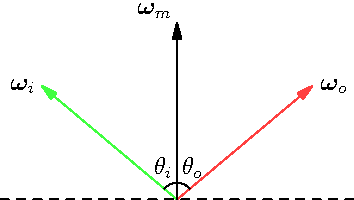
\includegraphics{asy/wm_reflect.pdf}
    \caption{Reflection}
    \label{fig:wm_reflect}
\end{subfigure}%
\begin{subfigure}{.5\textwidth}
    \centering
    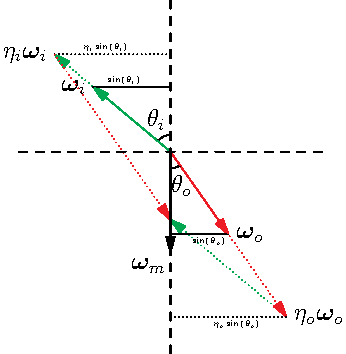
\includegraphics{asy/wm_refract.pdf}
    \caption{Refraction}
    \label{fig:wm_refract}
\end{subfigure}
\caption{
\textbf{(a)} For the reflective case, the halfvector $\wm$ lies simply in the middle of the incident and outgoing direction.
\textbf{(b)} We can obtain the halfvector $\wm$ for the refractive case by summing $\eta_i \wi$ and $\eta_o \wo$, where $\eta_i$ and $\eta_o$ are the indices of refraction of the incident and outgoing medium, respectively. The orthogonal components of $\wi$ and $\wo$ are simply the sine, so by weighting and summing them they cancel out according to Snell's law.
}
\end{figure}

For the specular component, I use the Torrance-Sparrow/Cook-Torrance microfacet model \bcite{torrance1967, cook1982} with the corrected normalization factor from \textcite{walter2007}:
\begin{equation}
    f_s(\wi, \vec{x}, \wo) = \frac{D(\NdotH) G(\n, \wi, \wo) F(\LdotH)}{4 \NdotL \NdotV}
\end{equation}
where $D$ is the isotropic Trowbridge-Reitz normal distribution function (NDF) originally defined by \textcite{trowbridge1975} and later rediscovered by \textcite{walter2007}:
\begin{equation}
    D(\NdotH) = \frac{\alpha^2}{\pi (\alpha^2 \cos^2 \theta_m + \sin^2 \theta_m)^2}
\end{equation}
Here, $\alpha$ is the width of the microfacet distribution, which is related to the roughness of the surface.
$\wm$ is the normal of an ideally reflecting microfacet (see \autoref{fig:wm_reflect}):
\begin{equation}
    \wm = \frac{\wi + \wo}{\|\wi + \wo\|}
\end{equation}

$G$ is the corresponding geometric attenuation term, for which I use the Smith shadowing-masking function \bcite{smith1967}, derived for the Trowbridge-Reitz NDF by \textcite{walter2007}:
\begin{equation}
    \begin{aligned}
    G(\n, \wi, \wo) &= \frac{1}{1 + \Lambda(\NdotL) + \Lambda(\NdotV)}\\
    \quad \text{with } \quad
    \Lambda(\NdotX) &= \frac{1}{2} \left( \sqrt{1 + \alpha^2 \mathrm{tan}^2 \theta} - 1 \right)
    \end{aligned}
\end{equation}

For the Fresnel term $F$, I use the Schlick approximation \bcite{schlick1994}:
\begin{equation}
    F(\LdotH) = F_0 + (1 - F_0) (1 - \LdotH)^5
\end{equation}

In the case of transmission, the normal of an ideally refracting microfacet is given by (see \autoref{fig:wm_refract}):
% TODO: Figure
\begin{equation}
    \wm = \pm\frac{\eta_i \wi + \eta_o \wo}{\|\eta_i \wi + \eta_o \wo\|} = \pm\frac{\eta \wi + \wo}{\|\eta \wi + \wo\|}
\end{equation}
where $\eta = \frac{\eta_i}{\eta_o}$ is the relative index of refraction (IOR).
The transmission component is then the following, as derived by \textcite{walter2007}:
\begin{equation}
    f_t(\wi, \vec{x}, \wo) = \rho_t \frac{D(\NdotH) G(\n, \wi, \wo) (1 - F(\LdotH))}{(\LdotH + \VdotH / \eta)^2} \left|\frac{\LdotH \VdotH}{\NdotL \NdotV}\right|
\end{equation}

For the diffuse component, I simply use the Lambertian reflectance model:
% TODO: (1-specular_albedo) should be right
\begin{equation}
    f_d(\wi, \vec{x}, \wo) = \frac{\rho_d}{\pi}
\end{equation}
Several other, more physically accurate, models have been proposed for the diffuse component, such as the microfacet-based Oren-Nayar reflectance model \bcite{oren1994} or the heuristic model from \textcite{burley2012}.
The Oren-Nayar model is rather computational expensive and not fully energy conserving, although these deficiencies can be mostly overcome by the improvements made by \textcite{fujii}.
Burley's model suffers also from energy conservation issues, but renormalized versions exist \bcite{lagarde2014}.
However, the Lambertian model has the nice property of being constant over the hemisphere, which can be advantageous for caching.

To parameterize the BSDF, I use a base color $\vec{c} \in [0, 1]^3$, a metallic factor $m \in [0, 1]$, a roughness factor $r \in [0, 1]$ and a transmission factor $t \in [0, 1]$, as follows:
\begin{equation}
    \begin{aligned}
        \alpha &= r^2 \\
        \rho_d &= (1 - m) \cdot (1 - t) \cdot \vec{c} \\
        \rho_t &= (1 - m) \cdot t \cdot \vec{c} \\
        F_0 &= 0.04 \cdot (1 - m) + \vec{c} \cdot m \\
    \end{aligned}
\end{equation}
Here, I assume the IOR of the surface to be $1.5$, which results in a specular reflectance at normal incidence of $F_0 = 0.04$.
For metals, the base color $\vec{c}$ is used directly as the $F_0$ to simulate wavelength dependent complex-valued IOR.

\section{Importance Sampling}

As aforementioned, the variance of a Monte Carlo estimator can be reduced by sampling the integral using a probability distribution that is as proportional to the integrand as possible.
Revisiting the rendering equation (\ref{eq:rendering_equation}), we first concentrate on sampling the term $f(\wi, \vec{x}, \wo) \cos(\theta_i)$ of the integrand.
Also sampling $L_i(\vec{x}, \wi)$ is not that easy, because to obtain $L_i$ we would need to solve the rendering equation again.
Yet, several approaches have been made to also take $L_i$ into account, notably direct light sampling \bcite{veach1997}, path guiding \bcite{muller2017,muller2019,lafortune1995,jensen1995} and ReSTIR \bcite{bitterli2020}.
For my reference pathtracer, I will only employ BSDF sampling and direct light sampling (\ref{sec:mis}).

For the diffuse component, as it is constant I only sample the cosine weighted hemisphere:
\begin{equation}
    p_d(\wi) = \frac{\cos(\theta_i)}{\pi} \quad \text{for } \wi \in \Omega
\end{equation}

For the specular and transmissive components, I sample the distribution of visible microfacet normals (VNDF) \bcite{heitz2014a} of the Trowbridge-Reitz NDF, which is given by:
\begin{equation}
    p_\mathrm{VNDF}(\wm \mid \wo) = \frac{G_1(\wo, \wm) D(\NdotH) |\VdotH|}{|\NdotV|}
\end{equation}
Sampling this instead of the NDF reduces the variance at grazing angles, where many microfacets are shadowed.
To sample the VNDF, I use the method proposed by \textcite{dupuy2023}, which improves upon the original method \bcite{heitz2014a} and its follow-up \bcite{heitz2018}.

To weigh the BSDF, the VNDF has first to be transformed into a probability distribution over the domain of incoming directions $\wi$ using the Jacobian of the reflection operator \bcite{walter2007}:
\begin{equation}
    \begin{aligned}
        \wi &= \reflect(\wo, \wm), \quad \wm \sim p_\mathrm{VNDF}(\wm \mid \wo)\\
        p_s(\wi \mid \wo)
        &= p_\mathrm{VNDF}(\wm \mid \wo) \left\|\frac{\partial \wm}{\partial \wi}\right\|
        = \frac{p_\mathrm{VNDF}(\wm \mid \wo)}{4|\VdotH|}
        = \frac{G_1(\wo, \wm) D(\NdotH)}{4|\NdotV|}
    \end{aligned}
\end{equation}
$\left\|\frac{\partial \wm}{\partial \wi}\right\|$ denotes the absolute value of the determinant of the Jacobian for the transform from $\wm$ to $\wi$ and was derived by \textcite{walter2007}.

For the transmission component, I use the same approach, but with the Jacobian of the refraction operator \bcite{walter2007}:
% TODO: TIR
\begin{equation}
    \begin{aligned}
        \wi &= \refract(\wo, \wm), \quad \wm \sim p_\mathrm{VNDF}(\wm \mid \wo)\\
        p_t(\wi \mid \wo)
        &= p_\mathrm{VNDF}(\wm \mid \wo) \left\|\frac{\partial \wm}{\partial \wi}\right\| \\
        &= p_\mathrm{VNDF}(\wm \mid \wo) \frac{\eta_i^2 |\LdotH|}{|\eta_i \LdotH + \eta_o \VdotH|^2} \\
        &= \frac{G_1(\wo, \wm) D(\NdotH) |\VdotH|}{|\NdotV|} \frac{|\LdotH|}{|\LdotH + \VdotH / \eta|^2} \\
        &= \frac{G_1(\wo, \wm) D(\NdotH) |\LdotH \VdotH|}{|\NdotV| |\LdotH + \VdotH / \eta|^2}
    \end{aligned}
\end{equation}

To combine these three sampling strategies, one can use Russian Roulette again.
To optimally weigh the sampling strategies, one can first precompute the relative luminance $Y$ of the directional albedo of the respective BSDF components, which is the expected value of the BSDF in a perfect white furnace environment.
However, for performance reasons, I only approximate these weights by using the Fresnel term of a perfectly smooth surface and the base colors:
\begin{equation}
    \begin{aligned}
        Y_d &= Y(\rho_d) &\quad
        Y_s &= Y(F(\NdotV)) &\quad
        Y_t &= Y(\rho_t) \\
% TODO
        % Y_t &= Y((1 - F(\NdotV)) \cdot \rho_t) \\
        P_d &= \frac{Y_d}{Y_d + Y_s + Y_t} &\quad
        P_s &= \frac{Y_s}{Y_d + Y_s + Y_t} &\quad
        P_t &= \frac{Y_t}{Y_d + Y_s + Y_t} \\
    \end{aligned}
\end{equation}
The combined sampling distribution is then given by:
\begin{equation}
    p(\wi \mid \wo) = P_d p_d(\wi) + P_s p_s(\wi \mid \wo) + P_t p_t(\wi \mid \wo)
\end{equation}

\section{Evaluation of the Weighted BSDF}

Most of the time, we do not need to evaluate the BSDF directly, but rather the weighted BSDF, which is given by:
\begin{equation}
    \begin{aligned}
        w(\wi, \vec{x}, \wo)
        &= \frac{f(\wi, \vec{x}, \wo) \cos(\theta_i)}{p(\wi \mid \wo)}\\
        &= \begin{cases}
            \frac{(f_d(\wi, \vec{x}, \wo) + f_s(\wi, \vec{x}, \wo)) \NdotL}{P_d p_d(\wi) + P_s p_s(\wi \mid \wo)} & \text{if } \NdotL \NdotV > 0 \\
            \frac{f_t(\wi, \vec{x}, \wo) \NdotL}{P_t p_t(\wi \mid \wo)} & \text{otherwise}
        \end{cases}
    \end{aligned}
\end{equation}

Using this formulation is more efficient because large parts cancel out, improving numerical stability and performance.
For the reflective part we then get:
\begin{equation}
    \begin{aligned}
        w_r{(\wi, \vec{x}, \wo)}
        &= \frac{(f_d(\wi, \vec{x}, \wo) + f_s(\wi, \vec{x}, \wo)) \NdotL}{P_d p_d(\wi) + P_s p_s(\wi \mid \wo)}
        = \frac{G_1^{-1} (k G^{-1} \rho_d + \pi D F)}{G^{-1} (k G_1^{-1} P_d + \pi D P_s)},\\
        k &= 4 \NdotL \NdotV
    \end{aligned}
\end{equation}

And for the transmissive part:
\begin{equation}
    \begin{aligned}
        w_t(\wi, \vec{x}, \wo)
        = \frac{f_t(\wi, \vec{x}, \wo) \NdotL}{P_t p_t(\wi \mid \wo)}
        = \rho_t \frac{G (1 - F)}{G_1 P_t}
        = \rho_t \frac{G_1^{-1} (1 - F)}{G^{-1} P_t}
    \end{aligned}
\end{equation}

I used the fact that $G$ and $G_1$ are both reciprocals to eliminate unnecessary divisions:
\begin{equation}
    \begin{aligned}
        G^{-1} = 1 + \Lambda(\NdotL) + \Lambda(\NdotV)\quad \text{and} \quad
        G_1^{-1} = 1 + \Lambda(\NdotV)
    \end{aligned}
\end{equation}

\section{Multiple Importance Sampling}
\label{sec:mis}

BSDF importance sampling already works well for glossy materials and diffuse lighting, when it comes to diffuse materials and direct lighting however, it has rather high variance and does not work at all for infinitesimal light sources.
In these scenarios, direct light sampling is much more efficient, which samples the light sources instead of the BSDF.

To maximize path reuse, a common strategy is to draw from both sampling strategies at every path vertex, using the BSDF sampling for path continuation and the light sampling for light collection.
This technique is called Next Event Estimation (NEE).

A general approach to combine multiple sampling strategies is given by the Multiple Importance Sampling (MIS) estimator, which was first introduced by \textcite{veach1997}:
\begin{equation}
    \estimator{I_\mathrm{MIS}} = \sum_{i=1}^{N} \frac{1}{N_i} \sum_{j=1}^{N_i} w_i(\hat{x}_{i,j}) \frac{f(\hat{x}_{i,j})}{p_i(\hat{x}_{i,j})}, \quad \hat{x}_{i,j} \sim p_i(\hat{x}_{i,j})
\end{equation}
where $N$ is the number of sampling strategies, $N_i$ is the number of samples drawn from the $i$-th sampling strategy, $p_i$ is the probability distribution of the $i$-th sampling strategy and $w_i(\hat{x})$ is the weight of the sample $\hat{x}$ drawn from the $i$-th sampling strategy with $\sum w_i(\hat{x}) = 1$.
This estimator is again trivially unbiased.

A naïve way to combine these two sampling strategies would be to simply weigh them equally.
However, this is suboptimal, as the resulting variance is then simply the average of the variances of both sampling strategies.
Instead, \textcite{veach1997} also introduced a provably optimal way to combine multiple sampling strategies, called the balance heuristic:
\begin{equation}
    w_i(\hat{x}) = \frac{N_i p_i(\hat{x})}{\sum_{j} N_j p_j(\hat{x})}
\end{equation}

Intuitively spoken, each sampling strategy is weighted according to how likely it is to produce the given sample.
Thus, a sample is weighted lower, if it is in an outlier of the generating distribution.

As suggested by \textcite{veach1997}, I use the power heuristic generalization with a sharpening exponent of $\beta=2$ to combine BSDF and light sampling:
\begin{equation}
    w_i^{\beta}(\hat{x}) = \frac{(N_i p_i(\hat{x}))^\beta}{\sum_{j} (N_j p_j(\hat{x}))^{\beta}}
\end{equation}
    
\chapter{Neural Radiance Caching}
\label{chap:nrc}

A weak point of the reference Monte Carlo pathtracer motivated in \ref{chap:pathtracing} is, that we have to start from zero, every time the scene or camera changes.
It would make sense to keep samples around that can be reused when temporally and spatially similar paths occur in the evaluation of the global illumination integral.
\textcite{muller2021} introduced Neural Radiance Caching (NRC) to address this problem.
The idea is to train a neural network on collected radiance samples and use it to accumulate and interpolate these samples online.

Essentially, the idea is, to replace the recursive path tracing integral with a neural estimate of the radiance when the variance along the path becomes too high.

\section{Network Architecture}

Because the network has to be trained and evaluated in real-time, \textcite{muller2021} propose to use a rather small hardware-accelerated network architecture.
They use a fully connected network with 5 hidden layers, with 64 neurons and ReLU activation each.
The output layer has 3 neurons, one for each color channel.
Additionally, they omit biases as they did not observe a measurable benefit and it simplifies the implementation.
Because of the shallow architecture, skip connections are not needed to preserve the gradient flow.

To maximize the inference and training performance, \textcite{muller2021} introduce a fully fused implementation of the network, which fully utilizes shared memory and per-thread registers.
For this, the whole network is implemented as a single CUDA kernel, with each block handling a batch of 128 64-dimensional input vectors and keeping the $64\times128$ activations in shared memory.
Each block then consists of 4 warps, computing 16 neuron activations of the network each by applying a $16\times64$ matrix multiplication and the element-wise activation function.
For this, the hardware accelerated $16\times16$ FP16 matrix multiplication instruction is used when available.
With this hardware-optimized implementation, \textcite{muller2021} achieve a speedup of $5\times$ to $10\times$ compared to the widely used TensorFlow framework \bcite{tensorflow} on large batch sizes corresponding to HD resolution.

\section{Input Encodings}

As shown by \textcite{ren2013}, parametrizing the network with the outgoing direction $\wo$ and the position $\mathbf{x}$ alone is not sufficient for an accurate representation of the radiance field.
Instead, it proves beneficial to include the surface normal $\mathbf{n}$, surface roughness $r$ and the expected diffuse and specular reflectance terms $\mathbf{F}_d$ and $\mathbf{F}_s$ as well.

\subsection{Instant Neural Graphic Primitives}

\subsection{One Blob and One Blob Diffuse Encoding}

\begin{figure}
    \centering
    %% Creator: Matplotlib, PGF backend
%%
%% To include the figure in your LaTeX document, write
%%   \input{<filename>.pgf}
%%
%% Make sure the required packages are loaded in your preamble
%%   \usepackage{pgf}
%%
%% Also ensure that all the required font packages are loaded; for instance,
%% the lmodern package is sometimes necessary when using math font.
%%   \usepackage{lmodern}
%%
%% Figures using additional raster images can only be included by \input if
%% they are in the same directory as the main LaTeX file. For loading figures
%% from other directories you can use the `import` package
%%   \usepackage{import}
%%
%% and then include the figures with
%%   \import{<path to file>}{<filename>.pgf}
%%
%% Matplotlib used the following preamble
%%   \def\mathdefault#1{#1}
%%   \everymath=\expandafter{\the\everymath\displaystyle}
%%   \IfFileExists{scrextend.sty}{
%%     \usepackage[fontsize=10.000000pt]{scrextend}
%%   }{
%%     \renewcommand{\normalsize}{\fontsize{10.000000}{12.000000}\selectfont}
%%     \normalsize
%%   }
%%   
%%   \ifdefined\pdftexversion\else  % non-pdftex case.
%%     \usepackage{fontspec}
%%     \setmainfont{DejaVuSerif.ttf}[Path=\detokenize{/opt/homebrew/Cellar/python-matplotlib/3.10.3/libexec/lib/python3.13/site-packages/matplotlib/mpl-data/fonts/ttf/}]
%%     \setsansfont{DejaVuSans.ttf}[Path=\detokenize{/opt/homebrew/Cellar/python-matplotlib/3.10.3/libexec/lib/python3.13/site-packages/matplotlib/mpl-data/fonts/ttf/}]
%%     \setmonofont{DejaVuSansMono.ttf}[Path=\detokenize{/opt/homebrew/Cellar/python-matplotlib/3.10.3/libexec/lib/python3.13/site-packages/matplotlib/mpl-data/fonts/ttf/}]
%%   \fi
%%   \makeatletter\@ifpackageloaded{underscore}{}{\usepackage[strings]{underscore}}\makeatother
%%
\begingroup%
\makeatletter%
\begin{pgfpicture}%
\pgfpathrectangle{\pgfpointorigin}{\pgfqpoint{4.539660in}{3.141564in}}%
\pgfusepath{use as bounding box, clip}%
\begin{pgfscope}%
\pgfsetbuttcap%
\pgfsetmiterjoin%
\definecolor{currentfill}{rgb}{1.000000,1.000000,1.000000}%
\pgfsetfillcolor{currentfill}%
\pgfsetlinewidth{0.000000pt}%
\definecolor{currentstroke}{rgb}{1.000000,1.000000,1.000000}%
\pgfsetstrokecolor{currentstroke}%
\pgfsetdash{}{0pt}%
\pgfpathmoveto{\pgfqpoint{0.000000in}{0.000000in}}%
\pgfpathlineto{\pgfqpoint{4.539660in}{0.000000in}}%
\pgfpathlineto{\pgfqpoint{4.539660in}{3.141564in}}%
\pgfpathlineto{\pgfqpoint{0.000000in}{3.141564in}}%
\pgfpathlineto{\pgfqpoint{0.000000in}{0.000000in}}%
\pgfpathclose%
\pgfusepath{fill}%
\end{pgfscope}%
\begin{pgfscope}%
\pgfsetbuttcap%
\pgfsetmiterjoin%
\definecolor{currentfill}{rgb}{1.000000,1.000000,1.000000}%
\pgfsetfillcolor{currentfill}%
\pgfsetlinewidth{0.000000pt}%
\definecolor{currentstroke}{rgb}{0.000000,0.000000,0.000000}%
\pgfsetstrokecolor{currentstroke}%
\pgfsetstrokeopacity{0.000000}%
\pgfsetdash{}{0pt}%
\pgfpathmoveto{\pgfqpoint{0.564660in}{0.521603in}}%
\pgfpathlineto{\pgfqpoint{4.439660in}{0.521603in}}%
\pgfpathlineto{\pgfqpoint{4.439660in}{2.831603in}}%
\pgfpathlineto{\pgfqpoint{0.564660in}{2.831603in}}%
\pgfpathlineto{\pgfqpoint{0.564660in}{0.521603in}}%
\pgfpathclose%
\pgfusepath{fill}%
\end{pgfscope}%
\begin{pgfscope}%
\pgfpathrectangle{\pgfqpoint{0.564660in}{0.521603in}}{\pgfqpoint{3.875000in}{2.310000in}}%
\pgfusepath{clip}%
\pgfsetrectcap%
\pgfsetroundjoin%
\pgfsetlinewidth{0.803000pt}%
\definecolor{currentstroke}{rgb}{0.690196,0.690196,0.690196}%
\pgfsetstrokecolor{currentstroke}%
\pgfsetdash{}{0pt}%
\pgfpathmoveto{\pgfqpoint{0.740797in}{0.521603in}}%
\pgfpathlineto{\pgfqpoint{0.740797in}{2.831603in}}%
\pgfusepath{stroke}%
\end{pgfscope}%
\begin{pgfscope}%
\pgfsetbuttcap%
\pgfsetroundjoin%
\definecolor{currentfill}{rgb}{0.000000,0.000000,0.000000}%
\pgfsetfillcolor{currentfill}%
\pgfsetlinewidth{0.803000pt}%
\definecolor{currentstroke}{rgb}{0.000000,0.000000,0.000000}%
\pgfsetstrokecolor{currentstroke}%
\pgfsetdash{}{0pt}%
\pgfsys@defobject{currentmarker}{\pgfqpoint{0.000000in}{-0.048611in}}{\pgfqpoint{0.000000in}{0.000000in}}{%
\pgfpathmoveto{\pgfqpoint{0.000000in}{0.000000in}}%
\pgfpathlineto{\pgfqpoint{0.000000in}{-0.048611in}}%
\pgfusepath{stroke,fill}%
}%
\begin{pgfscope}%
\pgfsys@transformshift{0.740797in}{0.521603in}%
\pgfsys@useobject{currentmarker}{}%
\end{pgfscope}%
\end{pgfscope}%
\begin{pgfscope}%
\definecolor{textcolor}{rgb}{0.000000,0.000000,0.000000}%
\pgfsetstrokecolor{textcolor}%
\pgfsetfillcolor{textcolor}%
\pgftext[x=0.740797in,y=0.424381in,,top]{\color{textcolor}{\rmfamily\fontsize{10.000000}{12.000000}\selectfont\catcode`\^=\active\def^{\ifmmode\sp\else\^{}\fi}\catcode`\%=\active\def%{\%}$\mathdefault{0.00}$}}%
\end{pgfscope}%
\begin{pgfscope}%
\pgfpathrectangle{\pgfqpoint{0.564660in}{0.521603in}}{\pgfqpoint{3.875000in}{2.310000in}}%
\pgfusepath{clip}%
\pgfsetrectcap%
\pgfsetroundjoin%
\pgfsetlinewidth{0.803000pt}%
\definecolor{currentstroke}{rgb}{0.690196,0.690196,0.690196}%
\pgfsetstrokecolor{currentstroke}%
\pgfsetdash{}{0pt}%
\pgfpathmoveto{\pgfqpoint{1.621478in}{0.521603in}}%
\pgfpathlineto{\pgfqpoint{1.621478in}{2.831603in}}%
\pgfusepath{stroke}%
\end{pgfscope}%
\begin{pgfscope}%
\pgfsetbuttcap%
\pgfsetroundjoin%
\definecolor{currentfill}{rgb}{0.000000,0.000000,0.000000}%
\pgfsetfillcolor{currentfill}%
\pgfsetlinewidth{0.803000pt}%
\definecolor{currentstroke}{rgb}{0.000000,0.000000,0.000000}%
\pgfsetstrokecolor{currentstroke}%
\pgfsetdash{}{0pt}%
\pgfsys@defobject{currentmarker}{\pgfqpoint{0.000000in}{-0.048611in}}{\pgfqpoint{0.000000in}{0.000000in}}{%
\pgfpathmoveto{\pgfqpoint{0.000000in}{0.000000in}}%
\pgfpathlineto{\pgfqpoint{0.000000in}{-0.048611in}}%
\pgfusepath{stroke,fill}%
}%
\begin{pgfscope}%
\pgfsys@transformshift{1.621478in}{0.521603in}%
\pgfsys@useobject{currentmarker}{}%
\end{pgfscope}%
\end{pgfscope}%
\begin{pgfscope}%
\definecolor{textcolor}{rgb}{0.000000,0.000000,0.000000}%
\pgfsetstrokecolor{textcolor}%
\pgfsetfillcolor{textcolor}%
\pgftext[x=1.621478in,y=0.424381in,,top]{\color{textcolor}{\rmfamily\fontsize{10.000000}{12.000000}\selectfont\catcode`\^=\active\def^{\ifmmode\sp\else\^{}\fi}\catcode`\%=\active\def%{\%}$\mathdefault{0.25}$}}%
\end{pgfscope}%
\begin{pgfscope}%
\pgfpathrectangle{\pgfqpoint{0.564660in}{0.521603in}}{\pgfqpoint{3.875000in}{2.310000in}}%
\pgfusepath{clip}%
\pgfsetrectcap%
\pgfsetroundjoin%
\pgfsetlinewidth{0.803000pt}%
\definecolor{currentstroke}{rgb}{0.690196,0.690196,0.690196}%
\pgfsetstrokecolor{currentstroke}%
\pgfsetdash{}{0pt}%
\pgfpathmoveto{\pgfqpoint{2.502160in}{0.521603in}}%
\pgfpathlineto{\pgfqpoint{2.502160in}{2.831603in}}%
\pgfusepath{stroke}%
\end{pgfscope}%
\begin{pgfscope}%
\pgfsetbuttcap%
\pgfsetroundjoin%
\definecolor{currentfill}{rgb}{0.000000,0.000000,0.000000}%
\pgfsetfillcolor{currentfill}%
\pgfsetlinewidth{0.803000pt}%
\definecolor{currentstroke}{rgb}{0.000000,0.000000,0.000000}%
\pgfsetstrokecolor{currentstroke}%
\pgfsetdash{}{0pt}%
\pgfsys@defobject{currentmarker}{\pgfqpoint{0.000000in}{-0.048611in}}{\pgfqpoint{0.000000in}{0.000000in}}{%
\pgfpathmoveto{\pgfqpoint{0.000000in}{0.000000in}}%
\pgfpathlineto{\pgfqpoint{0.000000in}{-0.048611in}}%
\pgfusepath{stroke,fill}%
}%
\begin{pgfscope}%
\pgfsys@transformshift{2.502160in}{0.521603in}%
\pgfsys@useobject{currentmarker}{}%
\end{pgfscope}%
\end{pgfscope}%
\begin{pgfscope}%
\definecolor{textcolor}{rgb}{0.000000,0.000000,0.000000}%
\pgfsetstrokecolor{textcolor}%
\pgfsetfillcolor{textcolor}%
\pgftext[x=2.502160in,y=0.424381in,,top]{\color{textcolor}{\rmfamily\fontsize{10.000000}{12.000000}\selectfont\catcode`\^=\active\def^{\ifmmode\sp\else\^{}\fi}\catcode`\%=\active\def%{\%}$\mathdefault{0.50}$}}%
\end{pgfscope}%
\begin{pgfscope}%
\pgfpathrectangle{\pgfqpoint{0.564660in}{0.521603in}}{\pgfqpoint{3.875000in}{2.310000in}}%
\pgfusepath{clip}%
\pgfsetrectcap%
\pgfsetroundjoin%
\pgfsetlinewidth{0.803000pt}%
\definecolor{currentstroke}{rgb}{0.690196,0.690196,0.690196}%
\pgfsetstrokecolor{currentstroke}%
\pgfsetdash{}{0pt}%
\pgfpathmoveto{\pgfqpoint{3.382842in}{0.521603in}}%
\pgfpathlineto{\pgfqpoint{3.382842in}{2.831603in}}%
\pgfusepath{stroke}%
\end{pgfscope}%
\begin{pgfscope}%
\pgfsetbuttcap%
\pgfsetroundjoin%
\definecolor{currentfill}{rgb}{0.000000,0.000000,0.000000}%
\pgfsetfillcolor{currentfill}%
\pgfsetlinewidth{0.803000pt}%
\definecolor{currentstroke}{rgb}{0.000000,0.000000,0.000000}%
\pgfsetstrokecolor{currentstroke}%
\pgfsetdash{}{0pt}%
\pgfsys@defobject{currentmarker}{\pgfqpoint{0.000000in}{-0.048611in}}{\pgfqpoint{0.000000in}{0.000000in}}{%
\pgfpathmoveto{\pgfqpoint{0.000000in}{0.000000in}}%
\pgfpathlineto{\pgfqpoint{0.000000in}{-0.048611in}}%
\pgfusepath{stroke,fill}%
}%
\begin{pgfscope}%
\pgfsys@transformshift{3.382842in}{0.521603in}%
\pgfsys@useobject{currentmarker}{}%
\end{pgfscope}%
\end{pgfscope}%
\begin{pgfscope}%
\definecolor{textcolor}{rgb}{0.000000,0.000000,0.000000}%
\pgfsetstrokecolor{textcolor}%
\pgfsetfillcolor{textcolor}%
\pgftext[x=3.382842in,y=0.424381in,,top]{\color{textcolor}{\rmfamily\fontsize{10.000000}{12.000000}\selectfont\catcode`\^=\active\def^{\ifmmode\sp\else\^{}\fi}\catcode`\%=\active\def%{\%}$\mathdefault{0.75}$}}%
\end{pgfscope}%
\begin{pgfscope}%
\pgfpathrectangle{\pgfqpoint{0.564660in}{0.521603in}}{\pgfqpoint{3.875000in}{2.310000in}}%
\pgfusepath{clip}%
\pgfsetrectcap%
\pgfsetroundjoin%
\pgfsetlinewidth{0.803000pt}%
\definecolor{currentstroke}{rgb}{0.690196,0.690196,0.690196}%
\pgfsetstrokecolor{currentstroke}%
\pgfsetdash{}{0pt}%
\pgfpathmoveto{\pgfqpoint{4.263524in}{0.521603in}}%
\pgfpathlineto{\pgfqpoint{4.263524in}{2.831603in}}%
\pgfusepath{stroke}%
\end{pgfscope}%
\begin{pgfscope}%
\pgfsetbuttcap%
\pgfsetroundjoin%
\definecolor{currentfill}{rgb}{0.000000,0.000000,0.000000}%
\pgfsetfillcolor{currentfill}%
\pgfsetlinewidth{0.803000pt}%
\definecolor{currentstroke}{rgb}{0.000000,0.000000,0.000000}%
\pgfsetstrokecolor{currentstroke}%
\pgfsetdash{}{0pt}%
\pgfsys@defobject{currentmarker}{\pgfqpoint{0.000000in}{-0.048611in}}{\pgfqpoint{0.000000in}{0.000000in}}{%
\pgfpathmoveto{\pgfqpoint{0.000000in}{0.000000in}}%
\pgfpathlineto{\pgfqpoint{0.000000in}{-0.048611in}}%
\pgfusepath{stroke,fill}%
}%
\begin{pgfscope}%
\pgfsys@transformshift{4.263524in}{0.521603in}%
\pgfsys@useobject{currentmarker}{}%
\end{pgfscope}%
\end{pgfscope}%
\begin{pgfscope}%
\definecolor{textcolor}{rgb}{0.000000,0.000000,0.000000}%
\pgfsetstrokecolor{textcolor}%
\pgfsetfillcolor{textcolor}%
\pgftext[x=4.263524in,y=0.424381in,,top]{\color{textcolor}{\rmfamily\fontsize{10.000000}{12.000000}\selectfont\catcode`\^=\active\def^{\ifmmode\sp\else\^{}\fi}\catcode`\%=\active\def%{\%}$\mathdefault{1.00}$}}%
\end{pgfscope}%
\begin{pgfscope}%
\definecolor{textcolor}{rgb}{0.000000,0.000000,0.000000}%
\pgfsetstrokecolor{textcolor}%
\pgfsetfillcolor{textcolor}%
\pgftext[x=2.502160in,y=0.234413in,,top]{\color{textcolor}{\rmfamily\fontsize{10.000000}{12.000000}\selectfont\catcode`\^=\active\def^{\ifmmode\sp\else\^{}\fi}\catcode`\%=\active\def%{\%}Input Position x}}%
\end{pgfscope}%
\begin{pgfscope}%
\pgfpathrectangle{\pgfqpoint{0.564660in}{0.521603in}}{\pgfqpoint{3.875000in}{2.310000in}}%
\pgfusepath{clip}%
\pgfsetrectcap%
\pgfsetroundjoin%
\pgfsetlinewidth{0.803000pt}%
\definecolor{currentstroke}{rgb}{0.690196,0.690196,0.690196}%
\pgfsetstrokecolor{currentstroke}%
\pgfsetdash{}{0pt}%
\pgfpathmoveto{\pgfqpoint{0.564660in}{0.626603in}}%
\pgfpathlineto{\pgfqpoint{4.439660in}{0.626603in}}%
\pgfusepath{stroke}%
\end{pgfscope}%
\begin{pgfscope}%
\pgfsetbuttcap%
\pgfsetroundjoin%
\definecolor{currentfill}{rgb}{0.000000,0.000000,0.000000}%
\pgfsetfillcolor{currentfill}%
\pgfsetlinewidth{0.803000pt}%
\definecolor{currentstroke}{rgb}{0.000000,0.000000,0.000000}%
\pgfsetstrokecolor{currentstroke}%
\pgfsetdash{}{0pt}%
\pgfsys@defobject{currentmarker}{\pgfqpoint{-0.048611in}{0.000000in}}{\pgfqpoint{-0.000000in}{0.000000in}}{%
\pgfpathmoveto{\pgfqpoint{-0.000000in}{0.000000in}}%
\pgfpathlineto{\pgfqpoint{-0.048611in}{0.000000in}}%
\pgfusepath{stroke,fill}%
}%
\begin{pgfscope}%
\pgfsys@transformshift{0.564660in}{0.626603in}%
\pgfsys@useobject{currentmarker}{}%
\end{pgfscope}%
\end{pgfscope}%
\begin{pgfscope}%
\definecolor{textcolor}{rgb}{0.000000,0.000000,0.000000}%
\pgfsetstrokecolor{textcolor}%
\pgfsetfillcolor{textcolor}%
\pgftext[x=0.289968in, y=0.573842in, left, base]{\color{textcolor}{\rmfamily\fontsize{10.000000}{12.000000}\selectfont\catcode`\^=\active\def^{\ifmmode\sp\else\^{}\fi}\catcode`\%=\active\def%{\%}$\mathdefault{0.0}$}}%
\end{pgfscope}%
\begin{pgfscope}%
\pgfpathrectangle{\pgfqpoint{0.564660in}{0.521603in}}{\pgfqpoint{3.875000in}{2.310000in}}%
\pgfusepath{clip}%
\pgfsetrectcap%
\pgfsetroundjoin%
\pgfsetlinewidth{0.803000pt}%
\definecolor{currentstroke}{rgb}{0.690196,0.690196,0.690196}%
\pgfsetstrokecolor{currentstroke}%
\pgfsetdash{}{0pt}%
\pgfpathmoveto{\pgfqpoint{0.564660in}{1.156282in}}%
\pgfpathlineto{\pgfqpoint{4.439660in}{1.156282in}}%
\pgfusepath{stroke}%
\end{pgfscope}%
\begin{pgfscope}%
\pgfsetbuttcap%
\pgfsetroundjoin%
\definecolor{currentfill}{rgb}{0.000000,0.000000,0.000000}%
\pgfsetfillcolor{currentfill}%
\pgfsetlinewidth{0.803000pt}%
\definecolor{currentstroke}{rgb}{0.000000,0.000000,0.000000}%
\pgfsetstrokecolor{currentstroke}%
\pgfsetdash{}{0pt}%
\pgfsys@defobject{currentmarker}{\pgfqpoint{-0.048611in}{0.000000in}}{\pgfqpoint{-0.000000in}{0.000000in}}{%
\pgfpathmoveto{\pgfqpoint{-0.000000in}{0.000000in}}%
\pgfpathlineto{\pgfqpoint{-0.048611in}{0.000000in}}%
\pgfusepath{stroke,fill}%
}%
\begin{pgfscope}%
\pgfsys@transformshift{0.564660in}{1.156282in}%
\pgfsys@useobject{currentmarker}{}%
\end{pgfscope}%
\end{pgfscope}%
\begin{pgfscope}%
\definecolor{textcolor}{rgb}{0.000000,0.000000,0.000000}%
\pgfsetstrokecolor{textcolor}%
\pgfsetfillcolor{textcolor}%
\pgftext[x=0.289968in, y=1.103521in, left, base]{\color{textcolor}{\rmfamily\fontsize{10.000000}{12.000000}\selectfont\catcode`\^=\active\def^{\ifmmode\sp\else\^{}\fi}\catcode`\%=\active\def%{\%}$\mathdefault{0.2}$}}%
\end{pgfscope}%
\begin{pgfscope}%
\pgfpathrectangle{\pgfqpoint{0.564660in}{0.521603in}}{\pgfqpoint{3.875000in}{2.310000in}}%
\pgfusepath{clip}%
\pgfsetrectcap%
\pgfsetroundjoin%
\pgfsetlinewidth{0.803000pt}%
\definecolor{currentstroke}{rgb}{0.690196,0.690196,0.690196}%
\pgfsetstrokecolor{currentstroke}%
\pgfsetdash{}{0pt}%
\pgfpathmoveto{\pgfqpoint{0.564660in}{1.685962in}}%
\pgfpathlineto{\pgfqpoint{4.439660in}{1.685962in}}%
\pgfusepath{stroke}%
\end{pgfscope}%
\begin{pgfscope}%
\pgfsetbuttcap%
\pgfsetroundjoin%
\definecolor{currentfill}{rgb}{0.000000,0.000000,0.000000}%
\pgfsetfillcolor{currentfill}%
\pgfsetlinewidth{0.803000pt}%
\definecolor{currentstroke}{rgb}{0.000000,0.000000,0.000000}%
\pgfsetstrokecolor{currentstroke}%
\pgfsetdash{}{0pt}%
\pgfsys@defobject{currentmarker}{\pgfqpoint{-0.048611in}{0.000000in}}{\pgfqpoint{-0.000000in}{0.000000in}}{%
\pgfpathmoveto{\pgfqpoint{-0.000000in}{0.000000in}}%
\pgfpathlineto{\pgfqpoint{-0.048611in}{0.000000in}}%
\pgfusepath{stroke,fill}%
}%
\begin{pgfscope}%
\pgfsys@transformshift{0.564660in}{1.685962in}%
\pgfsys@useobject{currentmarker}{}%
\end{pgfscope}%
\end{pgfscope}%
\begin{pgfscope}%
\definecolor{textcolor}{rgb}{0.000000,0.000000,0.000000}%
\pgfsetstrokecolor{textcolor}%
\pgfsetfillcolor{textcolor}%
\pgftext[x=0.289968in, y=1.633200in, left, base]{\color{textcolor}{\rmfamily\fontsize{10.000000}{12.000000}\selectfont\catcode`\^=\active\def^{\ifmmode\sp\else\^{}\fi}\catcode`\%=\active\def%{\%}$\mathdefault{0.4}$}}%
\end{pgfscope}%
\begin{pgfscope}%
\pgfpathrectangle{\pgfqpoint{0.564660in}{0.521603in}}{\pgfqpoint{3.875000in}{2.310000in}}%
\pgfusepath{clip}%
\pgfsetrectcap%
\pgfsetroundjoin%
\pgfsetlinewidth{0.803000pt}%
\definecolor{currentstroke}{rgb}{0.690196,0.690196,0.690196}%
\pgfsetstrokecolor{currentstroke}%
\pgfsetdash{}{0pt}%
\pgfpathmoveto{\pgfqpoint{0.564660in}{2.215641in}}%
\pgfpathlineto{\pgfqpoint{4.439660in}{2.215641in}}%
\pgfusepath{stroke}%
\end{pgfscope}%
\begin{pgfscope}%
\pgfsetbuttcap%
\pgfsetroundjoin%
\definecolor{currentfill}{rgb}{0.000000,0.000000,0.000000}%
\pgfsetfillcolor{currentfill}%
\pgfsetlinewidth{0.803000pt}%
\definecolor{currentstroke}{rgb}{0.000000,0.000000,0.000000}%
\pgfsetstrokecolor{currentstroke}%
\pgfsetdash{}{0pt}%
\pgfsys@defobject{currentmarker}{\pgfqpoint{-0.048611in}{0.000000in}}{\pgfqpoint{-0.000000in}{0.000000in}}{%
\pgfpathmoveto{\pgfqpoint{-0.000000in}{0.000000in}}%
\pgfpathlineto{\pgfqpoint{-0.048611in}{0.000000in}}%
\pgfusepath{stroke,fill}%
}%
\begin{pgfscope}%
\pgfsys@transformshift{0.564660in}{2.215641in}%
\pgfsys@useobject{currentmarker}{}%
\end{pgfscope}%
\end{pgfscope}%
\begin{pgfscope}%
\definecolor{textcolor}{rgb}{0.000000,0.000000,0.000000}%
\pgfsetstrokecolor{textcolor}%
\pgfsetfillcolor{textcolor}%
\pgftext[x=0.289968in, y=2.162879in, left, base]{\color{textcolor}{\rmfamily\fontsize{10.000000}{12.000000}\selectfont\catcode`\^=\active\def^{\ifmmode\sp\else\^{}\fi}\catcode`\%=\active\def%{\%}$\mathdefault{0.6}$}}%
\end{pgfscope}%
\begin{pgfscope}%
\pgfpathrectangle{\pgfqpoint{0.564660in}{0.521603in}}{\pgfqpoint{3.875000in}{2.310000in}}%
\pgfusepath{clip}%
\pgfsetrectcap%
\pgfsetroundjoin%
\pgfsetlinewidth{0.803000pt}%
\definecolor{currentstroke}{rgb}{0.690196,0.690196,0.690196}%
\pgfsetstrokecolor{currentstroke}%
\pgfsetdash{}{0pt}%
\pgfpathmoveto{\pgfqpoint{0.564660in}{2.745320in}}%
\pgfpathlineto{\pgfqpoint{4.439660in}{2.745320in}}%
\pgfusepath{stroke}%
\end{pgfscope}%
\begin{pgfscope}%
\pgfsetbuttcap%
\pgfsetroundjoin%
\definecolor{currentfill}{rgb}{0.000000,0.000000,0.000000}%
\pgfsetfillcolor{currentfill}%
\pgfsetlinewidth{0.803000pt}%
\definecolor{currentstroke}{rgb}{0.000000,0.000000,0.000000}%
\pgfsetstrokecolor{currentstroke}%
\pgfsetdash{}{0pt}%
\pgfsys@defobject{currentmarker}{\pgfqpoint{-0.048611in}{0.000000in}}{\pgfqpoint{-0.000000in}{0.000000in}}{%
\pgfpathmoveto{\pgfqpoint{-0.000000in}{0.000000in}}%
\pgfpathlineto{\pgfqpoint{-0.048611in}{0.000000in}}%
\pgfusepath{stroke,fill}%
}%
\begin{pgfscope}%
\pgfsys@transformshift{0.564660in}{2.745320in}%
\pgfsys@useobject{currentmarker}{}%
\end{pgfscope}%
\end{pgfscope}%
\begin{pgfscope}%
\definecolor{textcolor}{rgb}{0.000000,0.000000,0.000000}%
\pgfsetstrokecolor{textcolor}%
\pgfsetfillcolor{textcolor}%
\pgftext[x=0.289968in, y=2.692558in, left, base]{\color{textcolor}{\rmfamily\fontsize{10.000000}{12.000000}\selectfont\catcode`\^=\active\def^{\ifmmode\sp\else\^{}\fi}\catcode`\%=\active\def%{\%}$\mathdefault{0.8}$}}%
\end{pgfscope}%
\begin{pgfscope}%
\definecolor{textcolor}{rgb}{0.000000,0.000000,0.000000}%
\pgfsetstrokecolor{textcolor}%
\pgfsetfillcolor{textcolor}%
\pgftext[x=0.234413in,y=1.676603in,,bottom,rotate=90.000000]{\color{textcolor}{\rmfamily\fontsize{10.000000}{12.000000}\selectfont\catcode`\^=\active\def^{\ifmmode\sp\else\^{}\fi}\catcode`\%=\active\def%{\%}Bin Activation}}%
\end{pgfscope}%
\begin{pgfscope}%
\pgfpathrectangle{\pgfqpoint{0.564660in}{0.521603in}}{\pgfqpoint{3.875000in}{2.310000in}}%
\pgfusepath{clip}%
\pgfsetrectcap%
\pgfsetroundjoin%
\pgfsetlinewidth{1.505625pt}%
\definecolor{currentstroke}{rgb}{0.121569,0.466667,0.705882}%
\pgfsetstrokecolor{currentstroke}%
\pgfsetdash{}{0pt}%
\pgfpathmoveto{\pgfqpoint{0.740797in}{1.950801in}}%
\pgfpathlineto{\pgfqpoint{0.776380in}{2.050798in}}%
\pgfpathlineto{\pgfqpoint{0.811963in}{2.148923in}}%
\pgfpathlineto{\pgfqpoint{0.847546in}{2.243448in}}%
\pgfpathlineto{\pgfqpoint{0.883129in}{2.332805in}}%
\pgfpathlineto{\pgfqpoint{0.918712in}{2.415585in}}%
\pgfpathlineto{\pgfqpoint{0.954295in}{2.490537in}}%
\pgfpathlineto{\pgfqpoint{0.989878in}{2.556570in}}%
\pgfpathlineto{\pgfqpoint{1.025461in}{2.612750in}}%
\pgfpathlineto{\pgfqpoint{1.061045in}{2.658303in}}%
\pgfpathlineto{\pgfqpoint{1.096628in}{2.692615in}}%
\pgfpathlineto{\pgfqpoint{1.132211in}{2.715227in}}%
\pgfpathlineto{\pgfqpoint{1.167794in}{2.725843in}}%
\pgfpathlineto{\pgfqpoint{1.203377in}{2.724324in}}%
\pgfpathlineto{\pgfqpoint{1.238960in}{2.710690in}}%
\pgfpathlineto{\pgfqpoint{1.274543in}{2.685118in}}%
\pgfpathlineto{\pgfqpoint{1.310126in}{2.647947in}}%
\pgfpathlineto{\pgfqpoint{1.345709in}{2.599674in}}%
\pgfpathlineto{\pgfqpoint{1.381293in}{2.540951in}}%
\pgfpathlineto{\pgfqpoint{1.416876in}{2.472595in}}%
\pgfpathlineto{\pgfqpoint{1.452459in}{2.395578in}}%
\pgfpathlineto{\pgfqpoint{1.488042in}{2.311030in}}%
\pgfpathlineto{\pgfqpoint{1.523625in}{2.220242in}}%
\pgfpathlineto{\pgfqpoint{1.559208in}{2.124664in}}%
\pgfpathlineto{\pgfqpoint{1.594791in}{2.025904in}}%
\pgfpathlineto{\pgfqpoint{1.630374in}{1.925723in}}%
\pgfpathlineto{\pgfqpoint{1.665957in}{1.825617in}}%
\pgfpathlineto{\pgfqpoint{1.701540in}{1.726326in}}%
\pgfpathlineto{\pgfqpoint{1.737124in}{1.628496in}}%
\pgfpathlineto{\pgfqpoint{1.772707in}{1.532757in}}%
\pgfpathlineto{\pgfqpoint{1.808290in}{1.439717in}}%
\pgfpathlineto{\pgfqpoint{1.843873in}{1.349959in}}%
\pgfpathlineto{\pgfqpoint{1.879456in}{1.264030in}}%
\pgfpathlineto{\pgfqpoint{1.915039in}{1.182439in}}%
\pgfpathlineto{\pgfqpoint{1.950622in}{1.105648in}}%
\pgfpathlineto{\pgfqpoint{1.986205in}{1.034065in}}%
\pgfpathlineto{\pgfqpoint{2.021788in}{0.968040in}}%
\pgfpathlineto{\pgfqpoint{2.057371in}{0.907855in}}%
\pgfpathlineto{\pgfqpoint{2.092955in}{0.853722in}}%
\pgfpathlineto{\pgfqpoint{2.128538in}{0.805775in}}%
\pgfpathlineto{\pgfqpoint{2.164121in}{0.764060in}}%
\pgfpathlineto{\pgfqpoint{2.199704in}{0.728534in}}%
\pgfpathlineto{\pgfqpoint{2.235287in}{0.699055in}}%
\pgfpathlineto{\pgfqpoint{2.270870in}{0.675379in}}%
\pgfpathlineto{\pgfqpoint{2.306453in}{0.657147in}}%
\pgfpathlineto{\pgfqpoint{2.342036in}{0.643886in}}%
\pgfpathlineto{\pgfqpoint{2.377619in}{0.635001in}}%
\pgfpathlineto{\pgfqpoint{2.413203in}{0.629762in}}%
\pgfpathlineto{\pgfqpoint{2.448786in}{0.627307in}}%
\pgfpathlineto{\pgfqpoint{2.484369in}{0.626630in}}%
\pgfpathlineto{\pgfqpoint{2.519952in}{0.626603in}}%
\pgfpathlineto{\pgfqpoint{2.555535in}{0.626603in}}%
\pgfpathlineto{\pgfqpoint{2.591118in}{0.626603in}}%
\pgfpathlineto{\pgfqpoint{2.626701in}{0.626603in}}%
\pgfpathlineto{\pgfqpoint{2.662284in}{0.626603in}}%
\pgfpathlineto{\pgfqpoint{2.697867in}{0.626603in}}%
\pgfpathlineto{\pgfqpoint{2.733450in}{0.626603in}}%
\pgfpathlineto{\pgfqpoint{2.769034in}{0.626603in}}%
\pgfpathlineto{\pgfqpoint{2.804617in}{0.626603in}}%
\pgfpathlineto{\pgfqpoint{2.840200in}{0.626603in}}%
\pgfpathlineto{\pgfqpoint{2.875783in}{0.626603in}}%
\pgfpathlineto{\pgfqpoint{2.911366in}{0.626603in}}%
\pgfpathlineto{\pgfqpoint{2.946949in}{0.626603in}}%
\pgfpathlineto{\pgfqpoint{2.982532in}{0.626603in}}%
\pgfpathlineto{\pgfqpoint{3.018115in}{0.626603in}}%
\pgfpathlineto{\pgfqpoint{3.053698in}{0.626603in}}%
\pgfpathlineto{\pgfqpoint{3.089281in}{0.626603in}}%
\pgfpathlineto{\pgfqpoint{3.124865in}{0.626603in}}%
\pgfpathlineto{\pgfqpoint{3.160448in}{0.626603in}}%
\pgfpathlineto{\pgfqpoint{3.196031in}{0.626603in}}%
\pgfpathlineto{\pgfqpoint{3.231614in}{0.626603in}}%
\pgfpathlineto{\pgfqpoint{3.267197in}{0.626603in}}%
\pgfpathlineto{\pgfqpoint{3.302780in}{0.626603in}}%
\pgfpathlineto{\pgfqpoint{3.338363in}{0.626603in}}%
\pgfpathlineto{\pgfqpoint{3.373946in}{0.626603in}}%
\pgfpathlineto{\pgfqpoint{3.409529in}{0.626603in}}%
\pgfpathlineto{\pgfqpoint{3.445113in}{0.626603in}}%
\pgfpathlineto{\pgfqpoint{3.480696in}{0.626603in}}%
\pgfpathlineto{\pgfqpoint{3.516279in}{0.626603in}}%
\pgfpathlineto{\pgfqpoint{3.551862in}{0.626603in}}%
\pgfpathlineto{\pgfqpoint{3.587445in}{0.626603in}}%
\pgfpathlineto{\pgfqpoint{3.623028in}{0.626603in}}%
\pgfpathlineto{\pgfqpoint{3.658611in}{0.626603in}}%
\pgfpathlineto{\pgfqpoint{3.694194in}{0.626603in}}%
\pgfpathlineto{\pgfqpoint{3.729777in}{0.626603in}}%
\pgfpathlineto{\pgfqpoint{3.765360in}{0.626603in}}%
\pgfpathlineto{\pgfqpoint{3.800944in}{0.626603in}}%
\pgfpathlineto{\pgfqpoint{3.836527in}{0.626603in}}%
\pgfpathlineto{\pgfqpoint{3.872110in}{0.626603in}}%
\pgfpathlineto{\pgfqpoint{3.907693in}{0.626603in}}%
\pgfpathlineto{\pgfqpoint{3.943276in}{0.626603in}}%
\pgfpathlineto{\pgfqpoint{3.978859in}{0.626603in}}%
\pgfpathlineto{\pgfqpoint{4.014442in}{0.626603in}}%
\pgfpathlineto{\pgfqpoint{4.050025in}{0.626603in}}%
\pgfpathlineto{\pgfqpoint{4.085608in}{0.626603in}}%
\pgfpathlineto{\pgfqpoint{4.121191in}{0.626603in}}%
\pgfpathlineto{\pgfqpoint{4.156775in}{0.626603in}}%
\pgfpathlineto{\pgfqpoint{4.192358in}{0.626603in}}%
\pgfpathlineto{\pgfqpoint{4.227941in}{0.626603in}}%
\pgfpathlineto{\pgfqpoint{4.263524in}{0.626603in}}%
\pgfusepath{stroke}%
\end{pgfscope}%
\begin{pgfscope}%
\pgfpathrectangle{\pgfqpoint{0.564660in}{0.521603in}}{\pgfqpoint{3.875000in}{2.310000in}}%
\pgfusepath{clip}%
\pgfsetrectcap%
\pgfsetroundjoin%
\pgfsetlinewidth{1.505625pt}%
\definecolor{currentstroke}{rgb}{1.000000,0.498039,0.054902}%
\pgfsetstrokecolor{currentstroke}%
\pgfsetdash{}{0pt}%
\pgfpathmoveto{\pgfqpoint{0.740797in}{0.626603in}}%
\pgfpathlineto{\pgfqpoint{0.776380in}{0.626815in}}%
\pgfpathlineto{\pgfqpoint{0.811963in}{0.628246in}}%
\pgfpathlineto{\pgfqpoint{0.847546in}{0.631976in}}%
\pgfpathlineto{\pgfqpoint{0.883129in}{0.638939in}}%
\pgfpathlineto{\pgfqpoint{0.918712in}{0.649930in}}%
\pgfpathlineto{\pgfqpoint{0.954295in}{0.665609in}}%
\pgfpathlineto{\pgfqpoint{0.989878in}{0.686511in}}%
\pgfpathlineto{\pgfqpoint{1.025461in}{0.713052in}}%
\pgfpathlineto{\pgfqpoint{1.061045in}{0.745530in}}%
\pgfpathlineto{\pgfqpoint{1.096628in}{0.784139in}}%
\pgfpathlineto{\pgfqpoint{1.132211in}{0.828970in}}%
\pgfpathlineto{\pgfqpoint{1.167794in}{0.880022in}}%
\pgfpathlineto{\pgfqpoint{1.203377in}{0.937202in}}%
\pgfpathlineto{\pgfqpoint{1.238960in}{1.000338in}}%
\pgfpathlineto{\pgfqpoint{1.274543in}{1.069182in}}%
\pgfpathlineto{\pgfqpoint{1.310126in}{1.143417in}}%
\pgfpathlineto{\pgfqpoint{1.345709in}{1.222663in}}%
\pgfpathlineto{\pgfqpoint{1.381293in}{1.306483in}}%
\pgfpathlineto{\pgfqpoint{1.416876in}{1.394392in}}%
\pgfpathlineto{\pgfqpoint{1.452459in}{1.485862in}}%
\pgfpathlineto{\pgfqpoint{1.488042in}{1.580326in}}%
\pgfpathlineto{\pgfqpoint{1.523625in}{1.677189in}}%
\pgfpathlineto{\pgfqpoint{1.559208in}{1.775829in}}%
\pgfpathlineto{\pgfqpoint{1.594791in}{1.875609in}}%
\pgfpathlineto{\pgfqpoint{1.630374in}{1.975876in}}%
\pgfpathlineto{\pgfqpoint{1.665957in}{2.075575in}}%
\pgfpathlineto{\pgfqpoint{1.701540in}{2.172955in}}%
\pgfpathlineto{\pgfqpoint{1.737124in}{2.266329in}}%
\pgfpathlineto{\pgfqpoint{1.772707in}{2.354168in}}%
\pgfpathlineto{\pgfqpoint{1.808290in}{2.435102in}}%
\pgfpathlineto{\pgfqpoint{1.843873in}{2.507921in}}%
\pgfpathlineto{\pgfqpoint{1.879456in}{2.571571in}}%
\pgfpathlineto{\pgfqpoint{1.915039in}{2.625161in}}%
\pgfpathlineto{\pgfqpoint{1.950622in}{2.667956in}}%
\pgfpathlineto{\pgfqpoint{1.986205in}{2.699379in}}%
\pgfpathlineto{\pgfqpoint{2.021788in}{2.719014in}}%
\pgfpathlineto{\pgfqpoint{2.057371in}{2.726603in}}%
\pgfpathlineto{\pgfqpoint{2.092955in}{2.722047in}}%
\pgfpathlineto{\pgfqpoint{2.128538in}{2.705406in}}%
\pgfpathlineto{\pgfqpoint{2.164121in}{2.676896in}}%
\pgfpathlineto{\pgfqpoint{2.199704in}{2.636897in}}%
\pgfpathlineto{\pgfqpoint{2.235287in}{2.585943in}}%
\pgfpathlineto{\pgfqpoint{2.270870in}{2.524730in}}%
\pgfpathlineto{\pgfqpoint{2.306453in}{2.454111in}}%
\pgfpathlineto{\pgfqpoint{2.342036in}{2.375099in}}%
\pgfpathlineto{\pgfqpoint{2.377619in}{2.288864in}}%
\pgfpathlineto{\pgfqpoint{2.413203in}{2.196737in}}%
\pgfpathlineto{\pgfqpoint{2.448786in}{2.100206in}}%
\pgfpathlineto{\pgfqpoint{2.484369in}{2.000920in}}%
\pgfpathlineto{\pgfqpoint{2.519952in}{1.900656in}}%
\pgfpathlineto{\pgfqpoint{2.555535in}{1.800692in}}%
\pgfpathlineto{\pgfqpoint{2.591118in}{1.701707in}}%
\pgfpathlineto{\pgfqpoint{2.626701in}{1.604341in}}%
\pgfpathlineto{\pgfqpoint{2.662284in}{1.509220in}}%
\pgfpathlineto{\pgfqpoint{2.697867in}{1.416948in}}%
\pgfpathlineto{\pgfqpoint{2.733450in}{1.328097in}}%
\pgfpathlineto{\pgfqpoint{2.769034in}{1.243207in}}%
\pgfpathlineto{\pgfqpoint{2.804617in}{1.162775in}}%
\pgfpathlineto{\pgfqpoint{2.840200in}{1.087250in}}%
\pgfpathlineto{\pgfqpoint{2.875783in}{1.017026in}}%
\pgfpathlineto{\pgfqpoint{2.911366in}{0.952436in}}%
\pgfpathlineto{\pgfqpoint{2.946949in}{0.893748in}}%
\pgfpathlineto{\pgfqpoint{2.982532in}{0.841152in}}%
\pgfpathlineto{\pgfqpoint{3.018115in}{0.794762in}}%
\pgfpathlineto{\pgfqpoint{3.053698in}{0.754602in}}%
\pgfpathlineto{\pgfqpoint{3.089281in}{0.720605in}}%
\pgfpathlineto{\pgfqpoint{3.124865in}{0.692604in}}%
\pgfpathlineto{\pgfqpoint{3.160448in}{0.670327in}}%
\pgfpathlineto{\pgfqpoint{3.196031in}{0.653387in}}%
\pgfpathlineto{\pgfqpoint{3.231614in}{0.641281in}}%
\pgfpathlineto{\pgfqpoint{3.267197in}{0.633380in}}%
\pgfpathlineto{\pgfqpoint{3.302780in}{0.628924in}}%
\pgfpathlineto{\pgfqpoint{3.338363in}{0.627014in}}%
\pgfpathlineto{\pgfqpoint{3.373946in}{0.626607in}}%
\pgfpathlineto{\pgfqpoint{3.409529in}{0.626603in}}%
\pgfpathlineto{\pgfqpoint{3.445113in}{0.626603in}}%
\pgfpathlineto{\pgfqpoint{3.480696in}{0.626603in}}%
\pgfpathlineto{\pgfqpoint{3.516279in}{0.626603in}}%
\pgfpathlineto{\pgfqpoint{3.551862in}{0.626603in}}%
\pgfpathlineto{\pgfqpoint{3.587445in}{0.626603in}}%
\pgfpathlineto{\pgfqpoint{3.623028in}{0.626603in}}%
\pgfpathlineto{\pgfqpoint{3.658611in}{0.626603in}}%
\pgfpathlineto{\pgfqpoint{3.694194in}{0.626603in}}%
\pgfpathlineto{\pgfqpoint{3.729777in}{0.626603in}}%
\pgfpathlineto{\pgfqpoint{3.765360in}{0.626603in}}%
\pgfpathlineto{\pgfqpoint{3.800944in}{0.626603in}}%
\pgfpathlineto{\pgfqpoint{3.836527in}{0.626603in}}%
\pgfpathlineto{\pgfqpoint{3.872110in}{0.626603in}}%
\pgfpathlineto{\pgfqpoint{3.907693in}{0.626603in}}%
\pgfpathlineto{\pgfqpoint{3.943276in}{0.626603in}}%
\pgfpathlineto{\pgfqpoint{3.978859in}{0.626603in}}%
\pgfpathlineto{\pgfqpoint{4.014442in}{0.626603in}}%
\pgfpathlineto{\pgfqpoint{4.050025in}{0.626603in}}%
\pgfpathlineto{\pgfqpoint{4.085608in}{0.626603in}}%
\pgfpathlineto{\pgfqpoint{4.121191in}{0.626603in}}%
\pgfpathlineto{\pgfqpoint{4.156775in}{0.626603in}}%
\pgfpathlineto{\pgfqpoint{4.192358in}{0.626603in}}%
\pgfpathlineto{\pgfqpoint{4.227941in}{0.626603in}}%
\pgfpathlineto{\pgfqpoint{4.263524in}{0.626603in}}%
\pgfusepath{stroke}%
\end{pgfscope}%
\begin{pgfscope}%
\pgfpathrectangle{\pgfqpoint{0.564660in}{0.521603in}}{\pgfqpoint{3.875000in}{2.310000in}}%
\pgfusepath{clip}%
\pgfsetrectcap%
\pgfsetroundjoin%
\pgfsetlinewidth{1.505625pt}%
\definecolor{currentstroke}{rgb}{0.172549,0.627451,0.172549}%
\pgfsetstrokecolor{currentstroke}%
\pgfsetdash{}{0pt}%
\pgfpathmoveto{\pgfqpoint{0.740797in}{0.626603in}}%
\pgfpathlineto{\pgfqpoint{0.776380in}{0.626603in}}%
\pgfpathlineto{\pgfqpoint{0.811963in}{0.626603in}}%
\pgfpathlineto{\pgfqpoint{0.847546in}{0.626603in}}%
\pgfpathlineto{\pgfqpoint{0.883129in}{0.626603in}}%
\pgfpathlineto{\pgfqpoint{0.918712in}{0.626603in}}%
\pgfpathlineto{\pgfqpoint{0.954295in}{0.626603in}}%
\pgfpathlineto{\pgfqpoint{0.989878in}{0.626603in}}%
\pgfpathlineto{\pgfqpoint{1.025461in}{0.626603in}}%
\pgfpathlineto{\pgfqpoint{1.061045in}{0.626603in}}%
\pgfpathlineto{\pgfqpoint{1.096628in}{0.626603in}}%
\pgfpathlineto{\pgfqpoint{1.132211in}{0.626603in}}%
\pgfpathlineto{\pgfqpoint{1.167794in}{0.626603in}}%
\pgfpathlineto{\pgfqpoint{1.203377in}{0.626603in}}%
\pgfpathlineto{\pgfqpoint{1.238960in}{0.626603in}}%
\pgfpathlineto{\pgfqpoint{1.274543in}{0.626603in}}%
\pgfpathlineto{\pgfqpoint{1.310126in}{0.626603in}}%
\pgfpathlineto{\pgfqpoint{1.345709in}{0.626603in}}%
\pgfpathlineto{\pgfqpoint{1.381293in}{0.626603in}}%
\pgfpathlineto{\pgfqpoint{1.416876in}{0.626603in}}%
\pgfpathlineto{\pgfqpoint{1.452459in}{0.626603in}}%
\pgfpathlineto{\pgfqpoint{1.488042in}{0.626603in}}%
\pgfpathlineto{\pgfqpoint{1.523625in}{0.626603in}}%
\pgfpathlineto{\pgfqpoint{1.559208in}{0.626603in}}%
\pgfpathlineto{\pgfqpoint{1.594791in}{0.626603in}}%
\pgfpathlineto{\pgfqpoint{1.630374in}{0.626607in}}%
\pgfpathlineto{\pgfqpoint{1.665957in}{0.627014in}}%
\pgfpathlineto{\pgfqpoint{1.701540in}{0.628924in}}%
\pgfpathlineto{\pgfqpoint{1.737124in}{0.633380in}}%
\pgfpathlineto{\pgfqpoint{1.772707in}{0.641281in}}%
\pgfpathlineto{\pgfqpoint{1.808290in}{0.653387in}}%
\pgfpathlineto{\pgfqpoint{1.843873in}{0.670327in}}%
\pgfpathlineto{\pgfqpoint{1.879456in}{0.692604in}}%
\pgfpathlineto{\pgfqpoint{1.915039in}{0.720605in}}%
\pgfpathlineto{\pgfqpoint{1.950622in}{0.754602in}}%
\pgfpathlineto{\pgfqpoint{1.986205in}{0.794762in}}%
\pgfpathlineto{\pgfqpoint{2.021788in}{0.841152in}}%
\pgfpathlineto{\pgfqpoint{2.057371in}{0.893748in}}%
\pgfpathlineto{\pgfqpoint{2.092955in}{0.952436in}}%
\pgfpathlineto{\pgfqpoint{2.128538in}{1.017026in}}%
\pgfpathlineto{\pgfqpoint{2.164121in}{1.087250in}}%
\pgfpathlineto{\pgfqpoint{2.199704in}{1.162775in}}%
\pgfpathlineto{\pgfqpoint{2.235287in}{1.243207in}}%
\pgfpathlineto{\pgfqpoint{2.270870in}{1.328097in}}%
\pgfpathlineto{\pgfqpoint{2.306453in}{1.416948in}}%
\pgfpathlineto{\pgfqpoint{2.342036in}{1.509220in}}%
\pgfpathlineto{\pgfqpoint{2.377619in}{1.604341in}}%
\pgfpathlineto{\pgfqpoint{2.413203in}{1.701707in}}%
\pgfpathlineto{\pgfqpoint{2.448786in}{1.800692in}}%
\pgfpathlineto{\pgfqpoint{2.484369in}{1.900656in}}%
\pgfpathlineto{\pgfqpoint{2.519952in}{2.000920in}}%
\pgfpathlineto{\pgfqpoint{2.555535in}{2.100206in}}%
\pgfpathlineto{\pgfqpoint{2.591118in}{2.196737in}}%
\pgfpathlineto{\pgfqpoint{2.626701in}{2.288864in}}%
\pgfpathlineto{\pgfqpoint{2.662284in}{2.375099in}}%
\pgfpathlineto{\pgfqpoint{2.697867in}{2.454111in}}%
\pgfpathlineto{\pgfqpoint{2.733450in}{2.524730in}}%
\pgfpathlineto{\pgfqpoint{2.769034in}{2.585943in}}%
\pgfpathlineto{\pgfqpoint{2.804617in}{2.636897in}}%
\pgfpathlineto{\pgfqpoint{2.840200in}{2.676896in}}%
\pgfpathlineto{\pgfqpoint{2.875783in}{2.705406in}}%
\pgfpathlineto{\pgfqpoint{2.911366in}{2.722047in}}%
\pgfpathlineto{\pgfqpoint{2.946949in}{2.726603in}}%
\pgfpathlineto{\pgfqpoint{2.982532in}{2.719014in}}%
\pgfpathlineto{\pgfqpoint{3.018115in}{2.699379in}}%
\pgfpathlineto{\pgfqpoint{3.053698in}{2.667956in}}%
\pgfpathlineto{\pgfqpoint{3.089281in}{2.625161in}}%
\pgfpathlineto{\pgfqpoint{3.124865in}{2.571571in}}%
\pgfpathlineto{\pgfqpoint{3.160448in}{2.507921in}}%
\pgfpathlineto{\pgfqpoint{3.196031in}{2.435102in}}%
\pgfpathlineto{\pgfqpoint{3.231614in}{2.354168in}}%
\pgfpathlineto{\pgfqpoint{3.267197in}{2.266329in}}%
\pgfpathlineto{\pgfqpoint{3.302780in}{2.172955in}}%
\pgfpathlineto{\pgfqpoint{3.338363in}{2.075575in}}%
\pgfpathlineto{\pgfqpoint{3.373946in}{1.975876in}}%
\pgfpathlineto{\pgfqpoint{3.409529in}{1.875609in}}%
\pgfpathlineto{\pgfqpoint{3.445113in}{1.775829in}}%
\pgfpathlineto{\pgfqpoint{3.480696in}{1.677189in}}%
\pgfpathlineto{\pgfqpoint{3.516279in}{1.580326in}}%
\pgfpathlineto{\pgfqpoint{3.551862in}{1.485862in}}%
\pgfpathlineto{\pgfqpoint{3.587445in}{1.394392in}}%
\pgfpathlineto{\pgfqpoint{3.623028in}{1.306483in}}%
\pgfpathlineto{\pgfqpoint{3.658611in}{1.222663in}}%
\pgfpathlineto{\pgfqpoint{3.694194in}{1.143417in}}%
\pgfpathlineto{\pgfqpoint{3.729777in}{1.069182in}}%
\pgfpathlineto{\pgfqpoint{3.765360in}{1.000338in}}%
\pgfpathlineto{\pgfqpoint{3.800944in}{0.937202in}}%
\pgfpathlineto{\pgfqpoint{3.836527in}{0.880022in}}%
\pgfpathlineto{\pgfqpoint{3.872110in}{0.828970in}}%
\pgfpathlineto{\pgfqpoint{3.907693in}{0.784139in}}%
\pgfpathlineto{\pgfqpoint{3.943276in}{0.745530in}}%
\pgfpathlineto{\pgfqpoint{3.978859in}{0.713052in}}%
\pgfpathlineto{\pgfqpoint{4.014442in}{0.686511in}}%
\pgfpathlineto{\pgfqpoint{4.050025in}{0.665609in}}%
\pgfpathlineto{\pgfqpoint{4.085608in}{0.649930in}}%
\pgfpathlineto{\pgfqpoint{4.121191in}{0.638939in}}%
\pgfpathlineto{\pgfqpoint{4.156775in}{0.631976in}}%
\pgfpathlineto{\pgfqpoint{4.192358in}{0.628246in}}%
\pgfpathlineto{\pgfqpoint{4.227941in}{0.626815in}}%
\pgfpathlineto{\pgfqpoint{4.263524in}{0.626603in}}%
\pgfusepath{stroke}%
\end{pgfscope}%
\begin{pgfscope}%
\pgfpathrectangle{\pgfqpoint{0.564660in}{0.521603in}}{\pgfqpoint{3.875000in}{2.310000in}}%
\pgfusepath{clip}%
\pgfsetrectcap%
\pgfsetroundjoin%
\pgfsetlinewidth{1.505625pt}%
\definecolor{currentstroke}{rgb}{0.839216,0.152941,0.156863}%
\pgfsetstrokecolor{currentstroke}%
\pgfsetdash{}{0pt}%
\pgfpathmoveto{\pgfqpoint{0.740797in}{0.626603in}}%
\pgfpathlineto{\pgfqpoint{0.776380in}{0.626603in}}%
\pgfpathlineto{\pgfqpoint{0.811963in}{0.626603in}}%
\pgfpathlineto{\pgfqpoint{0.847546in}{0.626603in}}%
\pgfpathlineto{\pgfqpoint{0.883129in}{0.626603in}}%
\pgfpathlineto{\pgfqpoint{0.918712in}{0.626603in}}%
\pgfpathlineto{\pgfqpoint{0.954295in}{0.626603in}}%
\pgfpathlineto{\pgfqpoint{0.989878in}{0.626603in}}%
\pgfpathlineto{\pgfqpoint{1.025461in}{0.626603in}}%
\pgfpathlineto{\pgfqpoint{1.061045in}{0.626603in}}%
\pgfpathlineto{\pgfqpoint{1.096628in}{0.626603in}}%
\pgfpathlineto{\pgfqpoint{1.132211in}{0.626603in}}%
\pgfpathlineto{\pgfqpoint{1.167794in}{0.626603in}}%
\pgfpathlineto{\pgfqpoint{1.203377in}{0.626603in}}%
\pgfpathlineto{\pgfqpoint{1.238960in}{0.626603in}}%
\pgfpathlineto{\pgfqpoint{1.274543in}{0.626603in}}%
\pgfpathlineto{\pgfqpoint{1.310126in}{0.626603in}}%
\pgfpathlineto{\pgfqpoint{1.345709in}{0.626603in}}%
\pgfpathlineto{\pgfqpoint{1.381293in}{0.626603in}}%
\pgfpathlineto{\pgfqpoint{1.416876in}{0.626603in}}%
\pgfpathlineto{\pgfqpoint{1.452459in}{0.626603in}}%
\pgfpathlineto{\pgfqpoint{1.488042in}{0.626603in}}%
\pgfpathlineto{\pgfqpoint{1.523625in}{0.626603in}}%
\pgfpathlineto{\pgfqpoint{1.559208in}{0.626603in}}%
\pgfpathlineto{\pgfqpoint{1.594791in}{0.626603in}}%
\pgfpathlineto{\pgfqpoint{1.630374in}{0.626603in}}%
\pgfpathlineto{\pgfqpoint{1.665957in}{0.626603in}}%
\pgfpathlineto{\pgfqpoint{1.701540in}{0.626603in}}%
\pgfpathlineto{\pgfqpoint{1.737124in}{0.626603in}}%
\pgfpathlineto{\pgfqpoint{1.772707in}{0.626603in}}%
\pgfpathlineto{\pgfqpoint{1.808290in}{0.626603in}}%
\pgfpathlineto{\pgfqpoint{1.843873in}{0.626603in}}%
\pgfpathlineto{\pgfqpoint{1.879456in}{0.626603in}}%
\pgfpathlineto{\pgfqpoint{1.915039in}{0.626603in}}%
\pgfpathlineto{\pgfqpoint{1.950622in}{0.626603in}}%
\pgfpathlineto{\pgfqpoint{1.986205in}{0.626603in}}%
\pgfpathlineto{\pgfqpoint{2.021788in}{0.626603in}}%
\pgfpathlineto{\pgfqpoint{2.057371in}{0.626603in}}%
\pgfpathlineto{\pgfqpoint{2.092955in}{0.626603in}}%
\pgfpathlineto{\pgfqpoint{2.128538in}{0.626603in}}%
\pgfpathlineto{\pgfqpoint{2.164121in}{0.626603in}}%
\pgfpathlineto{\pgfqpoint{2.199704in}{0.626603in}}%
\pgfpathlineto{\pgfqpoint{2.235287in}{0.626603in}}%
\pgfpathlineto{\pgfqpoint{2.270870in}{0.626603in}}%
\pgfpathlineto{\pgfqpoint{2.306453in}{0.626603in}}%
\pgfpathlineto{\pgfqpoint{2.342036in}{0.626603in}}%
\pgfpathlineto{\pgfqpoint{2.377619in}{0.626603in}}%
\pgfpathlineto{\pgfqpoint{2.413203in}{0.626603in}}%
\pgfpathlineto{\pgfqpoint{2.448786in}{0.626603in}}%
\pgfpathlineto{\pgfqpoint{2.484369in}{0.626603in}}%
\pgfpathlineto{\pgfqpoint{2.519952in}{0.626630in}}%
\pgfpathlineto{\pgfqpoint{2.555535in}{0.627307in}}%
\pgfpathlineto{\pgfqpoint{2.591118in}{0.629762in}}%
\pgfpathlineto{\pgfqpoint{2.626701in}{0.635001in}}%
\pgfpathlineto{\pgfqpoint{2.662284in}{0.643886in}}%
\pgfpathlineto{\pgfqpoint{2.697867in}{0.657147in}}%
\pgfpathlineto{\pgfqpoint{2.733450in}{0.675379in}}%
\pgfpathlineto{\pgfqpoint{2.769034in}{0.699055in}}%
\pgfpathlineto{\pgfqpoint{2.804617in}{0.728534in}}%
\pgfpathlineto{\pgfqpoint{2.840200in}{0.764060in}}%
\pgfpathlineto{\pgfqpoint{2.875783in}{0.805775in}}%
\pgfpathlineto{\pgfqpoint{2.911366in}{0.853722in}}%
\pgfpathlineto{\pgfqpoint{2.946949in}{0.907855in}}%
\pgfpathlineto{\pgfqpoint{2.982532in}{0.968040in}}%
\pgfpathlineto{\pgfqpoint{3.018115in}{1.034065in}}%
\pgfpathlineto{\pgfqpoint{3.053698in}{1.105648in}}%
\pgfpathlineto{\pgfqpoint{3.089281in}{1.182439in}}%
\pgfpathlineto{\pgfqpoint{3.124865in}{1.264030in}}%
\pgfpathlineto{\pgfqpoint{3.160448in}{1.349959in}}%
\pgfpathlineto{\pgfqpoint{3.196031in}{1.439717in}}%
\pgfpathlineto{\pgfqpoint{3.231614in}{1.532757in}}%
\pgfpathlineto{\pgfqpoint{3.267197in}{1.628496in}}%
\pgfpathlineto{\pgfqpoint{3.302780in}{1.726326in}}%
\pgfpathlineto{\pgfqpoint{3.338363in}{1.825617in}}%
\pgfpathlineto{\pgfqpoint{3.373946in}{1.925723in}}%
\pgfpathlineto{\pgfqpoint{3.409529in}{2.025904in}}%
\pgfpathlineto{\pgfqpoint{3.445113in}{2.124664in}}%
\pgfpathlineto{\pgfqpoint{3.480696in}{2.220242in}}%
\pgfpathlineto{\pgfqpoint{3.516279in}{2.311030in}}%
\pgfpathlineto{\pgfqpoint{3.551862in}{2.395578in}}%
\pgfpathlineto{\pgfqpoint{3.587445in}{2.472595in}}%
\pgfpathlineto{\pgfqpoint{3.623028in}{2.540951in}}%
\pgfpathlineto{\pgfqpoint{3.658611in}{2.599674in}}%
\pgfpathlineto{\pgfqpoint{3.694194in}{2.647947in}}%
\pgfpathlineto{\pgfqpoint{3.729777in}{2.685118in}}%
\pgfpathlineto{\pgfqpoint{3.765360in}{2.710690in}}%
\pgfpathlineto{\pgfqpoint{3.800944in}{2.724324in}}%
\pgfpathlineto{\pgfqpoint{3.836527in}{2.725843in}}%
\pgfpathlineto{\pgfqpoint{3.872110in}{2.715227in}}%
\pgfpathlineto{\pgfqpoint{3.907693in}{2.692615in}}%
\pgfpathlineto{\pgfqpoint{3.943276in}{2.658303in}}%
\pgfpathlineto{\pgfqpoint{3.978859in}{2.612750in}}%
\pgfpathlineto{\pgfqpoint{4.014442in}{2.556570in}}%
\pgfpathlineto{\pgfqpoint{4.050025in}{2.490537in}}%
\pgfpathlineto{\pgfqpoint{4.085608in}{2.415585in}}%
\pgfpathlineto{\pgfqpoint{4.121191in}{2.332805in}}%
\pgfpathlineto{\pgfqpoint{4.156775in}{2.243448in}}%
\pgfpathlineto{\pgfqpoint{4.192358in}{2.148923in}}%
\pgfpathlineto{\pgfqpoint{4.227941in}{2.050798in}}%
\pgfpathlineto{\pgfqpoint{4.263524in}{1.950801in}}%
\pgfusepath{stroke}%
\end{pgfscope}%
\begin{pgfscope}%
\pgfsetrectcap%
\pgfsetmiterjoin%
\pgfsetlinewidth{0.803000pt}%
\definecolor{currentstroke}{rgb}{0.000000,0.000000,0.000000}%
\pgfsetstrokecolor{currentstroke}%
\pgfsetdash{}{0pt}%
\pgfpathmoveto{\pgfqpoint{0.564660in}{0.521603in}}%
\pgfpathlineto{\pgfqpoint{0.564660in}{2.831603in}}%
\pgfusepath{stroke}%
\end{pgfscope}%
\begin{pgfscope}%
\pgfsetrectcap%
\pgfsetmiterjoin%
\pgfsetlinewidth{0.803000pt}%
\definecolor{currentstroke}{rgb}{0.000000,0.000000,0.000000}%
\pgfsetstrokecolor{currentstroke}%
\pgfsetdash{}{0pt}%
\pgfpathmoveto{\pgfqpoint{4.439660in}{0.521603in}}%
\pgfpathlineto{\pgfqpoint{4.439660in}{2.831603in}}%
\pgfusepath{stroke}%
\end{pgfscope}%
\begin{pgfscope}%
\pgfsetrectcap%
\pgfsetmiterjoin%
\pgfsetlinewidth{0.803000pt}%
\definecolor{currentstroke}{rgb}{0.000000,0.000000,0.000000}%
\pgfsetstrokecolor{currentstroke}%
\pgfsetdash{}{0pt}%
\pgfpathmoveto{\pgfqpoint{0.564660in}{0.521603in}}%
\pgfpathlineto{\pgfqpoint{4.439660in}{0.521603in}}%
\pgfusepath{stroke}%
\end{pgfscope}%
\begin{pgfscope}%
\pgfsetrectcap%
\pgfsetmiterjoin%
\pgfsetlinewidth{0.803000pt}%
\definecolor{currentstroke}{rgb}{0.000000,0.000000,0.000000}%
\pgfsetstrokecolor{currentstroke}%
\pgfsetdash{}{0pt}%
\pgfpathmoveto{\pgfqpoint{0.564660in}{2.831603in}}%
\pgfpathlineto{\pgfqpoint{4.439660in}{2.831603in}}%
\pgfusepath{stroke}%
\end{pgfscope}%
\begin{pgfscope}%
\definecolor{textcolor}{rgb}{0.000000,0.000000,0.000000}%
\pgfsetstrokecolor{textcolor}%
\pgfsetfillcolor{textcolor}%
\pgftext[x=2.502160in,y=2.914937in,,base]{\color{textcolor}{\rmfamily\fontsize{12.000000}{14.400000}\selectfont\catcode`\^=\active\def^{\ifmmode\sp\else\^{}\fi}\catcode`\%=\active\def%{\%}Standard Quartic Bin Integration}}%
\end{pgfscope}%
\begin{pgfscope}%
\pgfsetbuttcap%
\pgfsetmiterjoin%
\definecolor{currentfill}{rgb}{1.000000,1.000000,1.000000}%
\pgfsetfillcolor{currentfill}%
\pgfsetfillopacity{0.800000}%
\pgfsetlinewidth{1.003750pt}%
\definecolor{currentstroke}{rgb}{0.800000,0.800000,0.800000}%
\pgfsetstrokecolor{currentstroke}%
\pgfsetstrokeopacity{0.800000}%
\pgfsetdash{}{0pt}%
\pgfpathmoveto{\pgfqpoint{3.470476in}{1.248056in}}%
\pgfpathlineto{\pgfqpoint{4.342438in}{1.248056in}}%
\pgfpathquadraticcurveto{\pgfqpoint{4.370216in}{1.248056in}}{\pgfqpoint{4.370216in}{1.275833in}}%
\pgfpathlineto{\pgfqpoint{4.370216in}{2.077373in}}%
\pgfpathquadraticcurveto{\pgfqpoint{4.370216in}{2.105151in}}{\pgfqpoint{4.342438in}{2.105151in}}%
\pgfpathlineto{\pgfqpoint{3.470476in}{2.105151in}}%
\pgfpathquadraticcurveto{\pgfqpoint{3.442698in}{2.105151in}}{\pgfqpoint{3.442698in}{2.077373in}}%
\pgfpathlineto{\pgfqpoint{3.442698in}{1.275833in}}%
\pgfpathquadraticcurveto{\pgfqpoint{3.442698in}{1.248056in}}{\pgfqpoint{3.470476in}{1.248056in}}%
\pgfpathlineto{\pgfqpoint{3.470476in}{1.248056in}}%
\pgfpathclose%
\pgfusepath{stroke,fill}%
\end{pgfscope}%
\begin{pgfscope}%
\pgfsetrectcap%
\pgfsetroundjoin%
\pgfsetlinewidth{1.505625pt}%
\definecolor{currentstroke}{rgb}{0.121569,0.466667,0.705882}%
\pgfsetstrokecolor{currentstroke}%
\pgfsetdash{}{0pt}%
\pgfpathmoveto{\pgfqpoint{3.498254in}{1.992684in}}%
\pgfpathlineto{\pgfqpoint{3.637143in}{1.992684in}}%
\pgfpathlineto{\pgfqpoint{3.776032in}{1.992684in}}%
\pgfusepath{stroke}%
\end{pgfscope}%
\begin{pgfscope}%
\definecolor{textcolor}{rgb}{0.000000,0.000000,0.000000}%
\pgfsetstrokecolor{textcolor}%
\pgfsetfillcolor{textcolor}%
\pgftext[x=3.887143in,y=1.944073in,left,base]{\color{textcolor}{\rmfamily\fontsize{10.000000}{12.000000}\selectfont\catcode`\^=\active\def^{\ifmmode\sp\else\^{}\fi}\catcode`\%=\active\def%{\%}bin=0}}%
\end{pgfscope}%
\begin{pgfscope}%
\pgfsetrectcap%
\pgfsetroundjoin%
\pgfsetlinewidth{1.505625pt}%
\definecolor{currentstroke}{rgb}{1.000000,0.498039,0.054902}%
\pgfsetstrokecolor{currentstroke}%
\pgfsetdash{}{0pt}%
\pgfpathmoveto{\pgfqpoint{3.498254in}{1.788826in}}%
\pgfpathlineto{\pgfqpoint{3.637143in}{1.788826in}}%
\pgfpathlineto{\pgfqpoint{3.776032in}{1.788826in}}%
\pgfusepath{stroke}%
\end{pgfscope}%
\begin{pgfscope}%
\definecolor{textcolor}{rgb}{0.000000,0.000000,0.000000}%
\pgfsetstrokecolor{textcolor}%
\pgfsetfillcolor{textcolor}%
\pgftext[x=3.887143in,y=1.740215in,left,base]{\color{textcolor}{\rmfamily\fontsize{10.000000}{12.000000}\selectfont\catcode`\^=\active\def^{\ifmmode\sp\else\^{}\fi}\catcode`\%=\active\def%{\%}bin=1}}%
\end{pgfscope}%
\begin{pgfscope}%
\pgfsetrectcap%
\pgfsetroundjoin%
\pgfsetlinewidth{1.505625pt}%
\definecolor{currentstroke}{rgb}{0.172549,0.627451,0.172549}%
\pgfsetstrokecolor{currentstroke}%
\pgfsetdash{}{0pt}%
\pgfpathmoveto{\pgfqpoint{3.498254in}{1.584969in}}%
\pgfpathlineto{\pgfqpoint{3.637143in}{1.584969in}}%
\pgfpathlineto{\pgfqpoint{3.776032in}{1.584969in}}%
\pgfusepath{stroke}%
\end{pgfscope}%
\begin{pgfscope}%
\definecolor{textcolor}{rgb}{0.000000,0.000000,0.000000}%
\pgfsetstrokecolor{textcolor}%
\pgfsetfillcolor{textcolor}%
\pgftext[x=3.887143in,y=1.536358in,left,base]{\color{textcolor}{\rmfamily\fontsize{10.000000}{12.000000}\selectfont\catcode`\^=\active\def^{\ifmmode\sp\else\^{}\fi}\catcode`\%=\active\def%{\%}bin=2}}%
\end{pgfscope}%
\begin{pgfscope}%
\pgfsetrectcap%
\pgfsetroundjoin%
\pgfsetlinewidth{1.505625pt}%
\definecolor{currentstroke}{rgb}{0.839216,0.152941,0.156863}%
\pgfsetstrokecolor{currentstroke}%
\pgfsetdash{}{0pt}%
\pgfpathmoveto{\pgfqpoint{3.498254in}{1.381112in}}%
\pgfpathlineto{\pgfqpoint{3.637143in}{1.381112in}}%
\pgfpathlineto{\pgfqpoint{3.776032in}{1.381112in}}%
\pgfusepath{stroke}%
\end{pgfscope}%
\begin{pgfscope}%
\definecolor{textcolor}{rgb}{0.000000,0.000000,0.000000}%
\pgfsetstrokecolor{textcolor}%
\pgfsetfillcolor{textcolor}%
\pgftext[x=3.887143in,y=1.332501in,left,base]{\color{textcolor}{\rmfamily\fontsize{10.000000}{12.000000}\selectfont\catcode`\^=\active\def^{\ifmmode\sp\else\^{}\fi}\catcode`\%=\active\def%{\%}bin=3}}%
\end{pgfscope}%
\end{pgfpicture}%
\makeatother%
\endgroup%

\end{figure}

\subsection{Reflected One Blob Octahedral Encoding}

\subsection{Reflectance Factorization}

\subsection{Emission Factorization}

\section{Training}

\subsection{Collecting Training Data}

To store the training data, I use a fixed-size ring buffer with an atomic counter to ensure thread safety.
This is not ideal, as it may lead to serialization of the GPU threads and thus potentially introduces a performance bottleneck, but it allows me to write dynamic amounts of data per thread.
Further research could be done to find a more efficient way to store the training data, for example using warp aggregation and compaction, but this is not straightforward as OptiX does not expose shared memory to allow for Shader Execution Reordering.

\subsection{Self-Learning}

\section{Inference}

\subsection{Temporal Stability}

\subsection{Path Termination Strategies}


    
\chapter{Bidirectional Radiance Caching}
\label{chap:bidirectional_caching}

\section{A General Theoretical Framework for Radiance Caching}
Before proposing new radiance caching techniques, I first want to take a step back and analyze radiance caching in general.

Radiance caching generally can be broken down into four steps:

\begin{enumerate}
    \item \textbf{Training}
    \begin{enumerate}
        \item \textbf{Query Prediction} First, we want to predict potential queries $\hat{q} = (\vec{x}, \vec{\omega}_o)$ according to a distribution $\hat{Q}(\hat{q})$.
        \item \textbf{Radiance Estimation} Given a predicted query $\hat{q}$, we want to estimate the outgoing radiance $L_o(\hat{q})$ at that query.
        For this, we can use any possible combination of radiance estimation techniques, such as path tracing, light tracing, photon mapping or Vertex Connection and Merging (VCM).
    \end{enumerate}
    \item \textbf{Inference}
    \begin{enumerate}
        \item \textbf{Query Sampling} We sample queries $q = (\vec{x}, \vec{\omega}_o)$ according to a distribution $Q(q)$.
        \item \textbf{Interpolation} Given a query $q$, we want to approximate the outgoing radiance $\hat{L}_o(q)$ by interpolating the radiance estimates of spatiotemporally nearby query predictions $\hat{q}$.
        We can use any interpolation or storing technique for this, such as nearest neighbor, linear interpolation or in our case the NRC.
        Note however, that this step generally introduces \textbf{bias}.
    \end{enumerate}
\end{enumerate}

\textbf{Note}, that using this framework we can observe that the \textbf{cache efficiency} is optimal if the query prediction distribution $\hat{Q}(\hat{q})$ is equal to the query sampling distribution $Q(q)$.
Conversely, if we sample a query $q^*$ that can not be predicted by the query predictor (i.e. $\hat{Q}(q^*)=0 \implies Q \not\subseteq \hat{Q}$), we introduce fundamental bias into the radiance cache $\hat{L}_o(q^*)$.

\textbf{Discussion:} It may be possible, to derive an unbiased radiance cache by storing the radiance estimates $L_o(\hat{q})$ in a spatial data structure and reconnecting the queries $q$ to the query predictions $\hat{q}$ similarly to Vertex Connection and Merging (VCM). % TODO: Check and cite

\section{Path Tracing}

\section{Light Tracing}

\section{Fully Connected Light Tracing}

\section{Balanced Light Tracing}

\section{Path Spaced Denoised Sparse Photon Mapping}

\section{Hardware Accelerated Vertex Connection and Merging}
    
\chapter{Results}
\label{chap:results}
For the purpose of reproducible evaluation, I have implemented a JSON-configurable CLI tool that was used to generate all results presented in this thesis and the exact parametrization is distributed along the source code on my repository \parencite{stamm2025}.
For the performance evaluation I use Cuda Events, tone mapping and blitting to the screen were not included into the measurements.

\begin{figure}
    \centering
    %% Creator: Matplotlib, PGF backend
%%
%% To include the figure in your LaTeX document, write
%%   \input{<filename>.pgf}
%%
%% Make sure the required packages are loaded in your preamble
%%   \usepackage{pgf}
%%
%% Also ensure that all the required font packages are loaded; for instance,
%% the lmodern package is sometimes necessary when using math font.
%%   \usepackage{lmodern}
%%
%% Figures using additional raster images can only be included by \input if
%% they are in the same directory as the main LaTeX file. For loading figures
%% from other directories you can use the `import` package
%%   \usepackage{import}
%%
%% and then include the figures with
%%   \import{<path to file>}{<filename>.pgf}
%%
%% Matplotlib used the following preamble
%%   \def\mathdefault#1{#1}
%%   \everymath=\expandafter{\the\everymath\displaystyle}
%%   \IfFileExists{scrextend.sty}{
%%     \usepackage[fontsize=10.000000pt]{scrextend}
%%   }{
%%     \renewcommand{\normalsize}{\fontsize{10.000000}{12.000000}\selectfont}
%%     \normalsize
%%   }
%%   
%%   \ifdefined\pdftexversion\else  % non-pdftex case.
%%     \usepackage{fontspec}
%%     \setmainfont{DejaVuSerif.ttf}[Path=\detokenize{/opt/homebrew/Cellar/python-matplotlib/3.10.5/libexec/lib/python3.13/site-packages/matplotlib/mpl-data/fonts/ttf/}]
%%     \setsansfont{DejaVuSans.ttf}[Path=\detokenize{/opt/homebrew/Cellar/python-matplotlib/3.10.5/libexec/lib/python3.13/site-packages/matplotlib/mpl-data/fonts/ttf/}]
%%     \setmonofont{DejaVuSansMono.ttf}[Path=\detokenize{/opt/homebrew/Cellar/python-matplotlib/3.10.5/libexec/lib/python3.13/site-packages/matplotlib/mpl-data/fonts/ttf/}]
%%   \fi
%%   \makeatletter\@ifpackageloaded{underscore}{}{\usepackage[strings]{underscore}}\makeatother
%%
\begingroup%
\makeatletter%
\begin{pgfpicture}%
\pgfpathrectangle{\pgfpointorigin}{\pgfqpoint{6.118122in}{3.116660in}}%
\pgfusepath{use as bounding box, clip}%
\begin{pgfscope}%
\pgfsetbuttcap%
\pgfsetmiterjoin%
\definecolor{currentfill}{rgb}{1.000000,1.000000,1.000000}%
\pgfsetfillcolor{currentfill}%
\pgfsetlinewidth{0.000000pt}%
\definecolor{currentstroke}{rgb}{1.000000,1.000000,1.000000}%
\pgfsetstrokecolor{currentstroke}%
\pgfsetdash{}{0pt}%
\pgfpathmoveto{\pgfqpoint{0.000000in}{0.000000in}}%
\pgfpathlineto{\pgfqpoint{6.118122in}{0.000000in}}%
\pgfpathlineto{\pgfqpoint{6.118122in}{3.116660in}}%
\pgfpathlineto{\pgfqpoint{0.000000in}{3.116660in}}%
\pgfpathlineto{\pgfqpoint{0.000000in}{0.000000in}}%
\pgfpathclose%
\pgfusepath{fill}%
\end{pgfscope}%
\begin{pgfscope}%
\pgfsetbuttcap%
\pgfsetmiterjoin%
\definecolor{currentfill}{rgb}{1.000000,1.000000,1.000000}%
\pgfsetfillcolor{currentfill}%
\pgfsetlinewidth{0.000000pt}%
\definecolor{currentstroke}{rgb}{0.000000,0.000000,0.000000}%
\pgfsetstrokecolor{currentstroke}%
\pgfsetstrokeopacity{0.000000}%
\pgfsetdash{}{0pt}%
\pgfpathmoveto{\pgfqpoint{2.060179in}{0.290505in}}%
\pgfpathlineto{\pgfqpoint{6.018122in}{0.290505in}}%
\pgfpathlineto{\pgfqpoint{6.018122in}{3.016660in}}%
\pgfpathlineto{\pgfqpoint{2.060179in}{3.016660in}}%
\pgfpathlineto{\pgfqpoint{2.060179in}{0.290505in}}%
\pgfpathclose%
\pgfusepath{fill}%
\end{pgfscope}%
\begin{pgfscope}%
\pgfpathrectangle{\pgfqpoint{2.060179in}{0.290505in}}{\pgfqpoint{3.957943in}{2.726155in}}%
\pgfusepath{clip}%
\pgfsetbuttcap%
\pgfsetmiterjoin%
\definecolor{currentfill}{rgb}{0.710588,0.710588,0.710588}%
\pgfsetfillcolor{currentfill}%
\pgfsetlinewidth{0.000000pt}%
\definecolor{currentstroke}{rgb}{0.000000,0.000000,0.000000}%
\pgfsetstrokecolor{currentstroke}%
\pgfsetstrokeopacity{0.000000}%
\pgfsetdash{}{0pt}%
\pgfpathmoveto{\pgfqpoint{2.240085in}{0.290505in}}%
\pgfpathlineto{\pgfqpoint{2.516864in}{0.290505in}}%
\pgfpathlineto{\pgfqpoint{2.516864in}{1.531982in}}%
\pgfpathlineto{\pgfqpoint{2.240085in}{1.531982in}}%
\pgfpathlineto{\pgfqpoint{2.240085in}{0.290505in}}%
\pgfpathclose%
\pgfusepath{fill}%
\end{pgfscope}%
\begin{pgfscope}%
\pgfpathrectangle{\pgfqpoint{2.060179in}{0.290505in}}{\pgfqpoint{3.957943in}{2.726155in}}%
\pgfusepath{clip}%
\pgfsetbuttcap%
\pgfsetmiterjoin%
\definecolor{currentfill}{rgb}{0.854902,0.439216,0.839216}%
\pgfsetfillcolor{currentfill}%
\pgfsetlinewidth{0.000000pt}%
\definecolor{currentstroke}{rgb}{0.000000,0.000000,0.000000}%
\pgfsetstrokecolor{currentstroke}%
\pgfsetstrokeopacity{0.000000}%
\pgfsetdash{}{0pt}%
\pgfpathmoveto{\pgfqpoint{2.240085in}{1.531982in}}%
\pgfpathlineto{\pgfqpoint{2.516864in}{1.531982in}}%
\pgfpathlineto{\pgfqpoint{2.516864in}{1.532932in}}%
\pgfpathlineto{\pgfqpoint{2.240085in}{1.532932in}}%
\pgfpathlineto{\pgfqpoint{2.240085in}{1.531982in}}%
\pgfpathclose%
\pgfusepath{fill}%
\end{pgfscope}%
\begin{pgfscope}%
\pgfpathrectangle{\pgfqpoint{2.060179in}{0.290505in}}{\pgfqpoint{3.957943in}{2.726155in}}%
\pgfusepath{clip}%
\pgfsetbuttcap%
\pgfsetmiterjoin%
\definecolor{currentfill}{rgb}{0.814118,0.883922,0.949804}%
\pgfsetfillcolor{currentfill}%
\pgfsetlinewidth{0.000000pt}%
\definecolor{currentstroke}{rgb}{0.000000,0.000000,0.000000}%
\pgfsetstrokecolor{currentstroke}%
\pgfsetstrokeopacity{0.000000}%
\pgfsetdash{}{0pt}%
\pgfpathmoveto{\pgfqpoint{2.793644in}{0.290505in}}%
\pgfpathlineto{\pgfqpoint{3.070423in}{0.290505in}}%
\pgfpathlineto{\pgfqpoint{3.070423in}{0.338908in}}%
\pgfpathlineto{\pgfqpoint{2.793644in}{0.338908in}}%
\pgfpathlineto{\pgfqpoint{2.793644in}{0.290505in}}%
\pgfpathclose%
\pgfusepath{fill}%
\end{pgfscope}%
\begin{pgfscope}%
\pgfpathrectangle{\pgfqpoint{2.060179in}{0.290505in}}{\pgfqpoint{3.957943in}{2.726155in}}%
\pgfusepath{clip}%
\pgfsetbuttcap%
\pgfsetmiterjoin%
\definecolor{currentfill}{rgb}{0.887059,0.887059,0.887059}%
\pgfsetfillcolor{currentfill}%
\pgfsetlinewidth{0.000000pt}%
\definecolor{currentstroke}{rgb}{0.000000,0.000000,0.000000}%
\pgfsetstrokecolor{currentstroke}%
\pgfsetstrokeopacity{0.000000}%
\pgfsetdash{}{0pt}%
\pgfpathmoveto{\pgfqpoint{2.793644in}{0.338908in}}%
\pgfpathlineto{\pgfqpoint{3.070423in}{0.338908in}}%
\pgfpathlineto{\pgfqpoint{3.070423in}{0.620419in}}%
\pgfpathlineto{\pgfqpoint{2.793644in}{0.620419in}}%
\pgfpathlineto{\pgfqpoint{2.793644in}{0.338908in}}%
\pgfpathclose%
\pgfusepath{fill}%
\end{pgfscope}%
\begin{pgfscope}%
\pgfpathrectangle{\pgfqpoint{2.060179in}{0.290505in}}{\pgfqpoint{3.957943in}{2.726155in}}%
\pgfusepath{clip}%
\pgfsetbuttcap%
\pgfsetmiterjoin%
\definecolor{currentfill}{rgb}{0.710588,0.710588,0.710588}%
\pgfsetfillcolor{currentfill}%
\pgfsetlinewidth{0.000000pt}%
\definecolor{currentstroke}{rgb}{0.000000,0.000000,0.000000}%
\pgfsetstrokecolor{currentstroke}%
\pgfsetstrokeopacity{0.000000}%
\pgfsetdash{}{0pt}%
\pgfpathmoveto{\pgfqpoint{2.793644in}{0.620419in}}%
\pgfpathlineto{\pgfqpoint{3.070423in}{0.620419in}}%
\pgfpathlineto{\pgfqpoint{3.070423in}{0.709444in}}%
\pgfpathlineto{\pgfqpoint{2.793644in}{0.709444in}}%
\pgfpathlineto{\pgfqpoint{2.793644in}{0.620419in}}%
\pgfpathclose%
\pgfusepath{fill}%
\end{pgfscope}%
\begin{pgfscope}%
\pgfpathrectangle{\pgfqpoint{2.060179in}{0.290505in}}{\pgfqpoint{3.957943in}{2.726155in}}%
\pgfusepath{clip}%
\pgfsetbuttcap%
\pgfsetmiterjoin%
\definecolor{currentfill}{rgb}{0.478431,0.478431,0.478431}%
\pgfsetfillcolor{currentfill}%
\pgfsetlinewidth{0.000000pt}%
\definecolor{currentstroke}{rgb}{0.000000,0.000000,0.000000}%
\pgfsetstrokecolor{currentstroke}%
\pgfsetstrokeopacity{0.000000}%
\pgfsetdash{}{0pt}%
\pgfpathmoveto{\pgfqpoint{2.793644in}{0.709444in}}%
\pgfpathlineto{\pgfqpoint{3.070423in}{0.709444in}}%
\pgfpathlineto{\pgfqpoint{3.070423in}{0.903746in}}%
\pgfpathlineto{\pgfqpoint{2.793644in}{0.903746in}}%
\pgfpathlineto{\pgfqpoint{2.793644in}{0.709444in}}%
\pgfpathclose%
\pgfusepath{fill}%
\end{pgfscope}%
\begin{pgfscope}%
\pgfpathrectangle{\pgfqpoint{2.060179in}{0.290505in}}{\pgfqpoint{3.957943in}{2.726155in}}%
\pgfusepath{clip}%
\pgfsetbuttcap%
\pgfsetmiterjoin%
\definecolor{currentfill}{rgb}{1.000000,0.752941,0.796078}%
\pgfsetfillcolor{currentfill}%
\pgfsetlinewidth{0.000000pt}%
\definecolor{currentstroke}{rgb}{0.000000,0.000000,0.000000}%
\pgfsetstrokecolor{currentstroke}%
\pgfsetstrokeopacity{0.000000}%
\pgfsetdash{}{0pt}%
\pgfpathmoveto{\pgfqpoint{2.793644in}{0.903746in}}%
\pgfpathlineto{\pgfqpoint{3.070423in}{0.903746in}}%
\pgfpathlineto{\pgfqpoint{3.070423in}{0.917474in}}%
\pgfpathlineto{\pgfqpoint{2.793644in}{0.917474in}}%
\pgfpathlineto{\pgfqpoint{2.793644in}{0.903746in}}%
\pgfpathclose%
\pgfusepath{fill}%
\end{pgfscope}%
\begin{pgfscope}%
\pgfpathrectangle{\pgfqpoint{2.060179in}{0.290505in}}{\pgfqpoint{3.957943in}{2.726155in}}%
\pgfusepath{clip}%
\pgfsetbuttcap%
\pgfsetmiterjoin%
\definecolor{currentfill}{rgb}{0.854902,0.439216,0.839216}%
\pgfsetfillcolor{currentfill}%
\pgfsetlinewidth{0.000000pt}%
\definecolor{currentstroke}{rgb}{0.000000,0.000000,0.000000}%
\pgfsetstrokecolor{currentstroke}%
\pgfsetstrokeopacity{0.000000}%
\pgfsetdash{}{0pt}%
\pgfpathmoveto{\pgfqpoint{2.793644in}{0.917474in}}%
\pgfpathlineto{\pgfqpoint{3.070423in}{0.917474in}}%
\pgfpathlineto{\pgfqpoint{3.070423in}{0.919898in}}%
\pgfpathlineto{\pgfqpoint{2.793644in}{0.919898in}}%
\pgfpathlineto{\pgfqpoint{2.793644in}{0.917474in}}%
\pgfpathclose%
\pgfusepath{fill}%
\end{pgfscope}%
\begin{pgfscope}%
\pgfpathrectangle{\pgfqpoint{2.060179in}{0.290505in}}{\pgfqpoint{3.957943in}{2.726155in}}%
\pgfusepath{clip}%
\pgfsetbuttcap%
\pgfsetmiterjoin%
\definecolor{currentfill}{rgb}{0.814118,0.883922,0.949804}%
\pgfsetfillcolor{currentfill}%
\pgfsetlinewidth{0.000000pt}%
\definecolor{currentstroke}{rgb}{0.000000,0.000000,0.000000}%
\pgfsetstrokecolor{currentstroke}%
\pgfsetstrokeopacity{0.000000}%
\pgfsetdash{}{0pt}%
\pgfpathmoveto{\pgfqpoint{3.347202in}{0.290505in}}%
\pgfpathlineto{\pgfqpoint{3.623981in}{0.290505in}}%
\pgfpathlineto{\pgfqpoint{3.623981in}{0.355218in}}%
\pgfpathlineto{\pgfqpoint{3.347202in}{0.355218in}}%
\pgfpathlineto{\pgfqpoint{3.347202in}{0.290505in}}%
\pgfpathclose%
\pgfusepath{fill}%
\end{pgfscope}%
\begin{pgfscope}%
\pgfpathrectangle{\pgfqpoint{2.060179in}{0.290505in}}{\pgfqpoint{3.957943in}{2.726155in}}%
\pgfusepath{clip}%
\pgfsetbuttcap%
\pgfsetmiterjoin%
\definecolor{currentfill}{rgb}{0.827451,0.932549,0.803137}%
\pgfsetfillcolor{currentfill}%
\pgfsetlinewidth{0.000000pt}%
\definecolor{currentstroke}{rgb}{0.000000,0.000000,0.000000}%
\pgfsetstrokecolor{currentstroke}%
\pgfsetstrokeopacity{0.000000}%
\pgfsetdash{}{0pt}%
\pgfpathmoveto{\pgfqpoint{3.347202in}{0.355218in}}%
\pgfpathlineto{\pgfqpoint{3.623981in}{0.355218in}}%
\pgfpathlineto{\pgfqpoint{3.623981in}{0.385085in}}%
\pgfpathlineto{\pgfqpoint{3.347202in}{0.385085in}}%
\pgfpathlineto{\pgfqpoint{3.347202in}{0.355218in}}%
\pgfpathclose%
\pgfusepath{fill}%
\end{pgfscope}%
\begin{pgfscope}%
\pgfpathrectangle{\pgfqpoint{2.060179in}{0.290505in}}{\pgfqpoint{3.957943in}{2.726155in}}%
\pgfusepath{clip}%
\pgfsetbuttcap%
\pgfsetmiterjoin%
\definecolor{currentfill}{rgb}{0.451765,0.767090,0.461207}%
\pgfsetfillcolor{currentfill}%
\pgfsetlinewidth{0.000000pt}%
\definecolor{currentstroke}{rgb}{0.000000,0.000000,0.000000}%
\pgfsetstrokecolor{currentstroke}%
\pgfsetstrokeopacity{0.000000}%
\pgfsetdash{}{0pt}%
\pgfpathmoveto{\pgfqpoint{3.347202in}{0.385085in}}%
\pgfpathlineto{\pgfqpoint{3.623981in}{0.385085in}}%
\pgfpathlineto{\pgfqpoint{3.623981in}{0.393893in}}%
\pgfpathlineto{\pgfqpoint{3.347202in}{0.393893in}}%
\pgfpathlineto{\pgfqpoint{3.347202in}{0.385085in}}%
\pgfpathclose%
\pgfusepath{fill}%
\end{pgfscope}%
\begin{pgfscope}%
\pgfpathrectangle{\pgfqpoint{2.060179in}{0.290505in}}{\pgfqpoint{3.957943in}{2.726155in}}%
\pgfusepath{clip}%
\pgfsetbuttcap%
\pgfsetmiterjoin%
\definecolor{currentfill}{rgb}{0.887059,0.887059,0.887059}%
\pgfsetfillcolor{currentfill}%
\pgfsetlinewidth{0.000000pt}%
\definecolor{currentstroke}{rgb}{0.000000,0.000000,0.000000}%
\pgfsetstrokecolor{currentstroke}%
\pgfsetstrokeopacity{0.000000}%
\pgfsetdash{}{0pt}%
\pgfpathmoveto{\pgfqpoint{3.347202in}{0.393893in}}%
\pgfpathlineto{\pgfqpoint{3.623981in}{0.393893in}}%
\pgfpathlineto{\pgfqpoint{3.623981in}{0.706840in}}%
\pgfpathlineto{\pgfqpoint{3.347202in}{0.706840in}}%
\pgfpathlineto{\pgfqpoint{3.347202in}{0.393893in}}%
\pgfpathclose%
\pgfusepath{fill}%
\end{pgfscope}%
\begin{pgfscope}%
\pgfpathrectangle{\pgfqpoint{2.060179in}{0.290505in}}{\pgfqpoint{3.957943in}{2.726155in}}%
\pgfusepath{clip}%
\pgfsetbuttcap%
\pgfsetmiterjoin%
\definecolor{currentfill}{rgb}{0.710588,0.710588,0.710588}%
\pgfsetfillcolor{currentfill}%
\pgfsetlinewidth{0.000000pt}%
\definecolor{currentstroke}{rgb}{0.000000,0.000000,0.000000}%
\pgfsetstrokecolor{currentstroke}%
\pgfsetstrokeopacity{0.000000}%
\pgfsetdash{}{0pt}%
\pgfpathmoveto{\pgfqpoint{3.347202in}{0.706840in}}%
\pgfpathlineto{\pgfqpoint{3.623981in}{0.706840in}}%
\pgfpathlineto{\pgfqpoint{3.623981in}{0.824404in}}%
\pgfpathlineto{\pgfqpoint{3.347202in}{0.824404in}}%
\pgfpathlineto{\pgfqpoint{3.347202in}{0.706840in}}%
\pgfpathclose%
\pgfusepath{fill}%
\end{pgfscope}%
\begin{pgfscope}%
\pgfpathrectangle{\pgfqpoint{2.060179in}{0.290505in}}{\pgfqpoint{3.957943in}{2.726155in}}%
\pgfusepath{clip}%
\pgfsetbuttcap%
\pgfsetmiterjoin%
\definecolor{currentfill}{rgb}{0.478431,0.478431,0.478431}%
\pgfsetfillcolor{currentfill}%
\pgfsetlinewidth{0.000000pt}%
\definecolor{currentstroke}{rgb}{0.000000,0.000000,0.000000}%
\pgfsetstrokecolor{currentstroke}%
\pgfsetstrokeopacity{0.000000}%
\pgfsetdash{}{0pt}%
\pgfpathmoveto{\pgfqpoint{3.347202in}{0.824404in}}%
\pgfpathlineto{\pgfqpoint{3.623981in}{0.824404in}}%
\pgfpathlineto{\pgfqpoint{3.623981in}{1.039657in}}%
\pgfpathlineto{\pgfqpoint{3.347202in}{1.039657in}}%
\pgfpathlineto{\pgfqpoint{3.347202in}{0.824404in}}%
\pgfpathclose%
\pgfusepath{fill}%
\end{pgfscope}%
\begin{pgfscope}%
\pgfpathrectangle{\pgfqpoint{2.060179in}{0.290505in}}{\pgfqpoint{3.957943in}{2.726155in}}%
\pgfusepath{clip}%
\pgfsetbuttcap%
\pgfsetmiterjoin%
\definecolor{currentfill}{rgb}{1.000000,0.752941,0.796078}%
\pgfsetfillcolor{currentfill}%
\pgfsetlinewidth{0.000000pt}%
\definecolor{currentstroke}{rgb}{0.000000,0.000000,0.000000}%
\pgfsetstrokecolor{currentstroke}%
\pgfsetstrokeopacity{0.000000}%
\pgfsetdash{}{0pt}%
\pgfpathmoveto{\pgfqpoint{3.347202in}{1.039657in}}%
\pgfpathlineto{\pgfqpoint{3.623981in}{1.039657in}}%
\pgfpathlineto{\pgfqpoint{3.623981in}{1.053399in}}%
\pgfpathlineto{\pgfqpoint{3.347202in}{1.053399in}}%
\pgfpathlineto{\pgfqpoint{3.347202in}{1.039657in}}%
\pgfpathclose%
\pgfusepath{fill}%
\end{pgfscope}%
\begin{pgfscope}%
\pgfpathrectangle{\pgfqpoint{2.060179in}{0.290505in}}{\pgfqpoint{3.957943in}{2.726155in}}%
\pgfusepath{clip}%
\pgfsetbuttcap%
\pgfsetmiterjoin%
\definecolor{currentfill}{rgb}{0.854902,0.439216,0.839216}%
\pgfsetfillcolor{currentfill}%
\pgfsetlinewidth{0.000000pt}%
\definecolor{currentstroke}{rgb}{0.000000,0.000000,0.000000}%
\pgfsetstrokecolor{currentstroke}%
\pgfsetstrokeopacity{0.000000}%
\pgfsetdash{}{0pt}%
\pgfpathmoveto{\pgfqpoint{3.347202in}{1.053399in}}%
\pgfpathlineto{\pgfqpoint{3.623981in}{1.053399in}}%
\pgfpathlineto{\pgfqpoint{3.623981in}{1.067114in}}%
\pgfpathlineto{\pgfqpoint{3.347202in}{1.067114in}}%
\pgfpathlineto{\pgfqpoint{3.347202in}{1.053399in}}%
\pgfpathclose%
\pgfusepath{fill}%
\end{pgfscope}%
\begin{pgfscope}%
\pgfpathrectangle{\pgfqpoint{2.060179in}{0.290505in}}{\pgfqpoint{3.957943in}{2.726155in}}%
\pgfusepath{clip}%
\pgfsetbuttcap%
\pgfsetmiterjoin%
\definecolor{currentfill}{rgb}{0.579608,0.770196,0.873725}%
\pgfsetfillcolor{currentfill}%
\pgfsetlinewidth{0.000000pt}%
\definecolor{currentstroke}{rgb}{0.000000,0.000000,0.000000}%
\pgfsetstrokecolor{currentstroke}%
\pgfsetstrokeopacity{0.000000}%
\pgfsetdash{}{0pt}%
\pgfpathmoveto{\pgfqpoint{3.900761in}{0.290505in}}%
\pgfpathlineto{\pgfqpoint{4.177540in}{0.290505in}}%
\pgfpathlineto{\pgfqpoint{4.177540in}{0.337256in}}%
\pgfpathlineto{\pgfqpoint{3.900761in}{0.337256in}}%
\pgfpathlineto{\pgfqpoint{3.900761in}{0.290505in}}%
\pgfpathclose%
\pgfusepath{fill}%
\end{pgfscope}%
\begin{pgfscope}%
\pgfpathrectangle{\pgfqpoint{2.060179in}{0.290505in}}{\pgfqpoint{3.957943in}{2.726155in}}%
\pgfusepath{clip}%
\pgfsetbuttcap%
\pgfsetmiterjoin%
\definecolor{currentfill}{rgb}{0.887059,0.887059,0.887059}%
\pgfsetfillcolor{currentfill}%
\pgfsetlinewidth{0.000000pt}%
\definecolor{currentstroke}{rgb}{0.000000,0.000000,0.000000}%
\pgfsetstrokecolor{currentstroke}%
\pgfsetstrokeopacity{0.000000}%
\pgfsetdash{}{0pt}%
\pgfpathmoveto{\pgfqpoint{3.900761in}{0.337256in}}%
\pgfpathlineto{\pgfqpoint{4.177540in}{0.337256in}}%
\pgfpathlineto{\pgfqpoint{4.177540in}{0.613994in}}%
\pgfpathlineto{\pgfqpoint{3.900761in}{0.613994in}}%
\pgfpathlineto{\pgfqpoint{3.900761in}{0.337256in}}%
\pgfpathclose%
\pgfusepath{fill}%
\end{pgfscope}%
\begin{pgfscope}%
\pgfpathrectangle{\pgfqpoint{2.060179in}{0.290505in}}{\pgfqpoint{3.957943in}{2.726155in}}%
\pgfusepath{clip}%
\pgfsetbuttcap%
\pgfsetmiterjoin%
\definecolor{currentfill}{rgb}{0.710588,0.710588,0.710588}%
\pgfsetfillcolor{currentfill}%
\pgfsetlinewidth{0.000000pt}%
\definecolor{currentstroke}{rgb}{0.000000,0.000000,0.000000}%
\pgfsetstrokecolor{currentstroke}%
\pgfsetstrokeopacity{0.000000}%
\pgfsetdash{}{0pt}%
\pgfpathmoveto{\pgfqpoint{3.900761in}{0.613994in}}%
\pgfpathlineto{\pgfqpoint{4.177540in}{0.613994in}}%
\pgfpathlineto{\pgfqpoint{4.177540in}{0.702965in}}%
\pgfpathlineto{\pgfqpoint{3.900761in}{0.702965in}}%
\pgfpathlineto{\pgfqpoint{3.900761in}{0.613994in}}%
\pgfpathclose%
\pgfusepath{fill}%
\end{pgfscope}%
\begin{pgfscope}%
\pgfpathrectangle{\pgfqpoint{2.060179in}{0.290505in}}{\pgfqpoint{3.957943in}{2.726155in}}%
\pgfusepath{clip}%
\pgfsetbuttcap%
\pgfsetmiterjoin%
\definecolor{currentfill}{rgb}{0.478431,0.478431,0.478431}%
\pgfsetfillcolor{currentfill}%
\pgfsetlinewidth{0.000000pt}%
\definecolor{currentstroke}{rgb}{0.000000,0.000000,0.000000}%
\pgfsetstrokecolor{currentstroke}%
\pgfsetstrokeopacity{0.000000}%
\pgfsetdash{}{0pt}%
\pgfpathmoveto{\pgfqpoint{3.900761in}{0.702965in}}%
\pgfpathlineto{\pgfqpoint{4.177540in}{0.702965in}}%
\pgfpathlineto{\pgfqpoint{4.177540in}{0.897140in}}%
\pgfpathlineto{\pgfqpoint{3.900761in}{0.897140in}}%
\pgfpathlineto{\pgfqpoint{3.900761in}{0.702965in}}%
\pgfpathclose%
\pgfusepath{fill}%
\end{pgfscope}%
\begin{pgfscope}%
\pgfpathrectangle{\pgfqpoint{2.060179in}{0.290505in}}{\pgfqpoint{3.957943in}{2.726155in}}%
\pgfusepath{clip}%
\pgfsetbuttcap%
\pgfsetmiterjoin%
\definecolor{currentfill}{rgb}{1.000000,0.752941,0.796078}%
\pgfsetfillcolor{currentfill}%
\pgfsetlinewidth{0.000000pt}%
\definecolor{currentstroke}{rgb}{0.000000,0.000000,0.000000}%
\pgfsetstrokecolor{currentstroke}%
\pgfsetstrokeopacity{0.000000}%
\pgfsetdash{}{0pt}%
\pgfpathmoveto{\pgfqpoint{3.900761in}{0.897140in}}%
\pgfpathlineto{\pgfqpoint{4.177540in}{0.897140in}}%
\pgfpathlineto{\pgfqpoint{4.177540in}{0.910873in}}%
\pgfpathlineto{\pgfqpoint{3.900761in}{0.910873in}}%
\pgfpathlineto{\pgfqpoint{3.900761in}{0.897140in}}%
\pgfpathclose%
\pgfusepath{fill}%
\end{pgfscope}%
\begin{pgfscope}%
\pgfpathrectangle{\pgfqpoint{2.060179in}{0.290505in}}{\pgfqpoint{3.957943in}{2.726155in}}%
\pgfusepath{clip}%
\pgfsetbuttcap%
\pgfsetmiterjoin%
\definecolor{currentfill}{rgb}{0.854902,0.439216,0.839216}%
\pgfsetfillcolor{currentfill}%
\pgfsetlinewidth{0.000000pt}%
\definecolor{currentstroke}{rgb}{0.000000,0.000000,0.000000}%
\pgfsetstrokecolor{currentstroke}%
\pgfsetstrokeopacity{0.000000}%
\pgfsetdash{}{0pt}%
\pgfpathmoveto{\pgfqpoint{3.900761in}{0.910873in}}%
\pgfpathlineto{\pgfqpoint{4.177540in}{0.910873in}}%
\pgfpathlineto{\pgfqpoint{4.177540in}{0.913381in}}%
\pgfpathlineto{\pgfqpoint{3.900761in}{0.913381in}}%
\pgfpathlineto{\pgfqpoint{3.900761in}{0.910873in}}%
\pgfpathclose%
\pgfusepath{fill}%
\end{pgfscope}%
\begin{pgfscope}%
\pgfpathrectangle{\pgfqpoint{2.060179in}{0.290505in}}{\pgfqpoint{3.957943in}{2.726155in}}%
\pgfusepath{clip}%
\pgfsetbuttcap%
\pgfsetmiterjoin%
\definecolor{currentfill}{rgb}{0.579608,0.770196,0.873725}%
\pgfsetfillcolor{currentfill}%
\pgfsetlinewidth{0.000000pt}%
\definecolor{currentstroke}{rgb}{0.000000,0.000000,0.000000}%
\pgfsetstrokecolor{currentstroke}%
\pgfsetstrokeopacity{0.000000}%
\pgfsetdash{}{0pt}%
\pgfpathmoveto{\pgfqpoint{4.454319in}{0.290505in}}%
\pgfpathlineto{\pgfqpoint{4.731098in}{0.290505in}}%
\pgfpathlineto{\pgfqpoint{4.731098in}{0.487897in}}%
\pgfpathlineto{\pgfqpoint{4.454319in}{0.487897in}}%
\pgfpathlineto{\pgfqpoint{4.454319in}{0.290505in}}%
\pgfpathclose%
\pgfusepath{fill}%
\end{pgfscope}%
\begin{pgfscope}%
\pgfpathrectangle{\pgfqpoint{2.060179in}{0.290505in}}{\pgfqpoint{3.957943in}{2.726155in}}%
\pgfusepath{clip}%
\pgfsetbuttcap%
\pgfsetmiterjoin%
\definecolor{currentfill}{rgb}{0.887059,0.887059,0.887059}%
\pgfsetfillcolor{currentfill}%
\pgfsetlinewidth{0.000000pt}%
\definecolor{currentstroke}{rgb}{0.000000,0.000000,0.000000}%
\pgfsetstrokecolor{currentstroke}%
\pgfsetstrokeopacity{0.000000}%
\pgfsetdash{}{0pt}%
\pgfpathmoveto{\pgfqpoint{4.454319in}{0.487897in}}%
\pgfpathlineto{\pgfqpoint{4.731098in}{0.487897in}}%
\pgfpathlineto{\pgfqpoint{4.731098in}{0.768069in}}%
\pgfpathlineto{\pgfqpoint{4.454319in}{0.768069in}}%
\pgfpathlineto{\pgfqpoint{4.454319in}{0.487897in}}%
\pgfpathclose%
\pgfusepath{fill}%
\end{pgfscope}%
\begin{pgfscope}%
\pgfpathrectangle{\pgfqpoint{2.060179in}{0.290505in}}{\pgfqpoint{3.957943in}{2.726155in}}%
\pgfusepath{clip}%
\pgfsetbuttcap%
\pgfsetmiterjoin%
\definecolor{currentfill}{rgb}{0.710588,0.710588,0.710588}%
\pgfsetfillcolor{currentfill}%
\pgfsetlinewidth{0.000000pt}%
\definecolor{currentstroke}{rgb}{0.000000,0.000000,0.000000}%
\pgfsetstrokecolor{currentstroke}%
\pgfsetstrokeopacity{0.000000}%
\pgfsetdash{}{0pt}%
\pgfpathmoveto{\pgfqpoint{4.454319in}{0.768069in}}%
\pgfpathlineto{\pgfqpoint{4.731098in}{0.768069in}}%
\pgfpathlineto{\pgfqpoint{4.731098in}{0.857112in}}%
\pgfpathlineto{\pgfqpoint{4.454319in}{0.857112in}}%
\pgfpathlineto{\pgfqpoint{4.454319in}{0.768069in}}%
\pgfpathclose%
\pgfusepath{fill}%
\end{pgfscope}%
\begin{pgfscope}%
\pgfpathrectangle{\pgfqpoint{2.060179in}{0.290505in}}{\pgfqpoint{3.957943in}{2.726155in}}%
\pgfusepath{clip}%
\pgfsetbuttcap%
\pgfsetmiterjoin%
\definecolor{currentfill}{rgb}{0.478431,0.478431,0.478431}%
\pgfsetfillcolor{currentfill}%
\pgfsetlinewidth{0.000000pt}%
\definecolor{currentstroke}{rgb}{0.000000,0.000000,0.000000}%
\pgfsetstrokecolor{currentstroke}%
\pgfsetstrokeopacity{0.000000}%
\pgfsetdash{}{0pt}%
\pgfpathmoveto{\pgfqpoint{4.454319in}{0.857112in}}%
\pgfpathlineto{\pgfqpoint{4.731098in}{0.857112in}}%
\pgfpathlineto{\pgfqpoint{4.731098in}{1.051332in}}%
\pgfpathlineto{\pgfqpoint{4.454319in}{1.051332in}}%
\pgfpathlineto{\pgfqpoint{4.454319in}{0.857112in}}%
\pgfpathclose%
\pgfusepath{fill}%
\end{pgfscope}%
\begin{pgfscope}%
\pgfpathrectangle{\pgfqpoint{2.060179in}{0.290505in}}{\pgfqpoint{3.957943in}{2.726155in}}%
\pgfusepath{clip}%
\pgfsetbuttcap%
\pgfsetmiterjoin%
\definecolor{currentfill}{rgb}{1.000000,0.752941,0.796078}%
\pgfsetfillcolor{currentfill}%
\pgfsetlinewidth{0.000000pt}%
\definecolor{currentstroke}{rgb}{0.000000,0.000000,0.000000}%
\pgfsetstrokecolor{currentstroke}%
\pgfsetstrokeopacity{0.000000}%
\pgfsetdash{}{0pt}%
\pgfpathmoveto{\pgfqpoint{4.454319in}{1.051332in}}%
\pgfpathlineto{\pgfqpoint{4.731098in}{1.051332in}}%
\pgfpathlineto{\pgfqpoint{4.731098in}{1.065057in}}%
\pgfpathlineto{\pgfqpoint{4.454319in}{1.065057in}}%
\pgfpathlineto{\pgfqpoint{4.454319in}{1.051332in}}%
\pgfpathclose%
\pgfusepath{fill}%
\end{pgfscope}%
\begin{pgfscope}%
\pgfpathrectangle{\pgfqpoint{2.060179in}{0.290505in}}{\pgfqpoint{3.957943in}{2.726155in}}%
\pgfusepath{clip}%
\pgfsetbuttcap%
\pgfsetmiterjoin%
\definecolor{currentfill}{rgb}{0.854902,0.439216,0.839216}%
\pgfsetfillcolor{currentfill}%
\pgfsetlinewidth{0.000000pt}%
\definecolor{currentstroke}{rgb}{0.000000,0.000000,0.000000}%
\pgfsetstrokecolor{currentstroke}%
\pgfsetstrokeopacity{0.000000}%
\pgfsetdash{}{0pt}%
\pgfpathmoveto{\pgfqpoint{4.454319in}{1.065057in}}%
\pgfpathlineto{\pgfqpoint{4.731098in}{1.065057in}}%
\pgfpathlineto{\pgfqpoint{4.731098in}{1.067490in}}%
\pgfpathlineto{\pgfqpoint{4.454319in}{1.067490in}}%
\pgfpathlineto{\pgfqpoint{4.454319in}{1.065057in}}%
\pgfpathclose%
\pgfusepath{fill}%
\end{pgfscope}%
\begin{pgfscope}%
\pgfpathrectangle{\pgfqpoint{2.060179in}{0.290505in}}{\pgfqpoint{3.957943in}{2.726155in}}%
\pgfusepath{clip}%
\pgfsetbuttcap%
\pgfsetmiterjoin%
\definecolor{currentfill}{rgb}{0.993725,0.850196,0.704314}%
\pgfsetfillcolor{currentfill}%
\pgfsetlinewidth{0.000000pt}%
\definecolor{currentstroke}{rgb}{0.000000,0.000000,0.000000}%
\pgfsetstrokecolor{currentstroke}%
\pgfsetstrokeopacity{0.000000}%
\pgfsetdash{}{0pt}%
\pgfpathmoveto{\pgfqpoint{5.007877in}{0.290505in}}%
\pgfpathlineto{\pgfqpoint{5.284657in}{0.290505in}}%
\pgfpathlineto{\pgfqpoint{5.284657in}{0.297129in}}%
\pgfpathlineto{\pgfqpoint{5.007877in}{0.297129in}}%
\pgfpathlineto{\pgfqpoint{5.007877in}{0.290505in}}%
\pgfpathclose%
\pgfusepath{fill}%
\end{pgfscope}%
\begin{pgfscope}%
\pgfpathrectangle{\pgfqpoint{2.060179in}{0.290505in}}{\pgfqpoint{3.957943in}{2.726155in}}%
\pgfusepath{clip}%
\pgfsetbuttcap%
\pgfsetmiterjoin%
\definecolor{currentfill}{rgb}{0.992157,0.710065,0.464437}%
\pgfsetfillcolor{currentfill}%
\pgfsetlinewidth{0.000000pt}%
\definecolor{currentstroke}{rgb}{0.000000,0.000000,0.000000}%
\pgfsetstrokecolor{currentstroke}%
\pgfsetstrokeopacity{0.000000}%
\pgfsetdash{}{0pt}%
\pgfpathmoveto{\pgfqpoint{5.007877in}{0.297129in}}%
\pgfpathlineto{\pgfqpoint{5.284657in}{0.297129in}}%
\pgfpathlineto{\pgfqpoint{5.284657in}{0.339028in}}%
\pgfpathlineto{\pgfqpoint{5.007877in}{0.339028in}}%
\pgfpathlineto{\pgfqpoint{5.007877in}{0.297129in}}%
\pgfpathclose%
\pgfusepath{fill}%
\end{pgfscope}%
\begin{pgfscope}%
\pgfpathrectangle{\pgfqpoint{2.060179in}{0.290505in}}{\pgfqpoint{3.957943in}{2.726155in}}%
\pgfusepath{clip}%
\pgfsetbuttcap%
\pgfsetmiterjoin%
\definecolor{currentfill}{rgb}{0.991419,0.550727,0.232772}%
\pgfsetfillcolor{currentfill}%
\pgfsetlinewidth{0.000000pt}%
\definecolor{currentstroke}{rgb}{0.000000,0.000000,0.000000}%
\pgfsetstrokecolor{currentstroke}%
\pgfsetstrokeopacity{0.000000}%
\pgfsetdash{}{0pt}%
\pgfpathmoveto{\pgfqpoint{5.007877in}{0.339028in}}%
\pgfpathlineto{\pgfqpoint{5.284657in}{0.339028in}}%
\pgfpathlineto{\pgfqpoint{5.284657in}{0.601046in}}%
\pgfpathlineto{\pgfqpoint{5.007877in}{0.601046in}}%
\pgfpathlineto{\pgfqpoint{5.007877in}{0.339028in}}%
\pgfpathclose%
\pgfusepath{fill}%
\end{pgfscope}%
\begin{pgfscope}%
\pgfpathrectangle{\pgfqpoint{2.060179in}{0.290505in}}{\pgfqpoint{3.957943in}{2.726155in}}%
\pgfusepath{clip}%
\pgfsetbuttcap%
\pgfsetmiterjoin%
\definecolor{currentfill}{rgb}{0.925536,0.384867,0.059839}%
\pgfsetfillcolor{currentfill}%
\pgfsetlinewidth{0.000000pt}%
\definecolor{currentstroke}{rgb}{0.000000,0.000000,0.000000}%
\pgfsetstrokecolor{currentstroke}%
\pgfsetstrokeopacity{0.000000}%
\pgfsetdash{}{0pt}%
\pgfpathmoveto{\pgfqpoint{5.007877in}{0.601046in}}%
\pgfpathlineto{\pgfqpoint{5.284657in}{0.601046in}}%
\pgfpathlineto{\pgfqpoint{5.284657in}{0.609503in}}%
\pgfpathlineto{\pgfqpoint{5.007877in}{0.609503in}}%
\pgfpathlineto{\pgfqpoint{5.007877in}{0.601046in}}%
\pgfpathclose%
\pgfusepath{fill}%
\end{pgfscope}%
\begin{pgfscope}%
\pgfpathrectangle{\pgfqpoint{2.060179in}{0.290505in}}{\pgfqpoint{3.957943in}{2.726155in}}%
\pgfusepath{clip}%
\pgfsetbuttcap%
\pgfsetmiterjoin%
\definecolor{currentfill}{rgb}{0.887059,0.887059,0.887059}%
\pgfsetfillcolor{currentfill}%
\pgfsetlinewidth{0.000000pt}%
\definecolor{currentstroke}{rgb}{0.000000,0.000000,0.000000}%
\pgfsetstrokecolor{currentstroke}%
\pgfsetstrokeopacity{0.000000}%
\pgfsetdash{}{0pt}%
\pgfpathmoveto{\pgfqpoint{5.007877in}{0.609503in}}%
\pgfpathlineto{\pgfqpoint{5.284657in}{0.609503in}}%
\pgfpathlineto{\pgfqpoint{5.284657in}{0.908102in}}%
\pgfpathlineto{\pgfqpoint{5.007877in}{0.908102in}}%
\pgfpathlineto{\pgfqpoint{5.007877in}{0.609503in}}%
\pgfpathclose%
\pgfusepath{fill}%
\end{pgfscope}%
\begin{pgfscope}%
\pgfpathrectangle{\pgfqpoint{2.060179in}{0.290505in}}{\pgfqpoint{3.957943in}{2.726155in}}%
\pgfusepath{clip}%
\pgfsetbuttcap%
\pgfsetmiterjoin%
\definecolor{currentfill}{rgb}{0.710588,0.710588,0.710588}%
\pgfsetfillcolor{currentfill}%
\pgfsetlinewidth{0.000000pt}%
\definecolor{currentstroke}{rgb}{0.000000,0.000000,0.000000}%
\pgfsetstrokecolor{currentstroke}%
\pgfsetstrokeopacity{0.000000}%
\pgfsetdash{}{0pt}%
\pgfpathmoveto{\pgfqpoint{5.007877in}{0.908102in}}%
\pgfpathlineto{\pgfqpoint{5.284657in}{0.908102in}}%
\pgfpathlineto{\pgfqpoint{5.284657in}{0.997261in}}%
\pgfpathlineto{\pgfqpoint{5.007877in}{0.997261in}}%
\pgfpathlineto{\pgfqpoint{5.007877in}{0.908102in}}%
\pgfpathclose%
\pgfusepath{fill}%
\end{pgfscope}%
\begin{pgfscope}%
\pgfpathrectangle{\pgfqpoint{2.060179in}{0.290505in}}{\pgfqpoint{3.957943in}{2.726155in}}%
\pgfusepath{clip}%
\pgfsetbuttcap%
\pgfsetmiterjoin%
\definecolor{currentfill}{rgb}{0.478431,0.478431,0.478431}%
\pgfsetfillcolor{currentfill}%
\pgfsetlinewidth{0.000000pt}%
\definecolor{currentstroke}{rgb}{0.000000,0.000000,0.000000}%
\pgfsetstrokecolor{currentstroke}%
\pgfsetstrokeopacity{0.000000}%
\pgfsetdash{}{0pt}%
\pgfpathmoveto{\pgfqpoint{5.007877in}{0.997261in}}%
\pgfpathlineto{\pgfqpoint{5.284657in}{0.997261in}}%
\pgfpathlineto{\pgfqpoint{5.284657in}{1.191919in}}%
\pgfpathlineto{\pgfqpoint{5.007877in}{1.191919in}}%
\pgfpathlineto{\pgfqpoint{5.007877in}{0.997261in}}%
\pgfpathclose%
\pgfusepath{fill}%
\end{pgfscope}%
\begin{pgfscope}%
\pgfpathrectangle{\pgfqpoint{2.060179in}{0.290505in}}{\pgfqpoint{3.957943in}{2.726155in}}%
\pgfusepath{clip}%
\pgfsetbuttcap%
\pgfsetmiterjoin%
\definecolor{currentfill}{rgb}{1.000000,0.752941,0.796078}%
\pgfsetfillcolor{currentfill}%
\pgfsetlinewidth{0.000000pt}%
\definecolor{currentstroke}{rgb}{0.000000,0.000000,0.000000}%
\pgfsetstrokecolor{currentstroke}%
\pgfsetstrokeopacity{0.000000}%
\pgfsetdash{}{0pt}%
\pgfpathmoveto{\pgfqpoint{5.007877in}{1.191919in}}%
\pgfpathlineto{\pgfqpoint{5.284657in}{1.191919in}}%
\pgfpathlineto{\pgfqpoint{5.284657in}{1.205650in}}%
\pgfpathlineto{\pgfqpoint{5.007877in}{1.205650in}}%
\pgfpathlineto{\pgfqpoint{5.007877in}{1.191919in}}%
\pgfpathclose%
\pgfusepath{fill}%
\end{pgfscope}%
\begin{pgfscope}%
\pgfpathrectangle{\pgfqpoint{2.060179in}{0.290505in}}{\pgfqpoint{3.957943in}{2.726155in}}%
\pgfusepath{clip}%
\pgfsetbuttcap%
\pgfsetmiterjoin%
\definecolor{currentfill}{rgb}{0.854902,0.439216,0.839216}%
\pgfsetfillcolor{currentfill}%
\pgfsetlinewidth{0.000000pt}%
\definecolor{currentstroke}{rgb}{0.000000,0.000000,0.000000}%
\pgfsetstrokecolor{currentstroke}%
\pgfsetstrokeopacity{0.000000}%
\pgfsetdash{}{0pt}%
\pgfpathmoveto{\pgfqpoint{5.007877in}{1.205650in}}%
\pgfpathlineto{\pgfqpoint{5.284657in}{1.205650in}}%
\pgfpathlineto{\pgfqpoint{5.284657in}{1.211475in}}%
\pgfpathlineto{\pgfqpoint{5.007877in}{1.211475in}}%
\pgfpathlineto{\pgfqpoint{5.007877in}{1.205650in}}%
\pgfpathclose%
\pgfusepath{fill}%
\end{pgfscope}%
\begin{pgfscope}%
\pgfpathrectangle{\pgfqpoint{2.060179in}{0.290505in}}{\pgfqpoint{3.957943in}{2.726155in}}%
\pgfusepath{clip}%
\pgfsetbuttcap%
\pgfsetmiterjoin%
\definecolor{currentfill}{rgb}{0.993725,0.850196,0.704314}%
\pgfsetfillcolor{currentfill}%
\pgfsetlinewidth{0.000000pt}%
\definecolor{currentstroke}{rgb}{0.000000,0.000000,0.000000}%
\pgfsetstrokecolor{currentstroke}%
\pgfsetstrokeopacity{0.000000}%
\pgfsetdash{}{0pt}%
\pgfpathmoveto{\pgfqpoint{5.561436in}{0.290505in}}%
\pgfpathlineto{\pgfqpoint{5.838215in}{0.290505in}}%
\pgfpathlineto{\pgfqpoint{5.838215in}{0.439441in}}%
\pgfpathlineto{\pgfqpoint{5.561436in}{0.439441in}}%
\pgfpathlineto{\pgfqpoint{5.561436in}{0.290505in}}%
\pgfpathclose%
\pgfusepath{fill}%
\end{pgfscope}%
\begin{pgfscope}%
\pgfpathrectangle{\pgfqpoint{2.060179in}{0.290505in}}{\pgfqpoint{3.957943in}{2.726155in}}%
\pgfusepath{clip}%
\pgfsetbuttcap%
\pgfsetmiterjoin%
\definecolor{currentfill}{rgb}{0.992157,0.710065,0.464437}%
\pgfsetfillcolor{currentfill}%
\pgfsetlinewidth{0.000000pt}%
\definecolor{currentstroke}{rgb}{0.000000,0.000000,0.000000}%
\pgfsetstrokecolor{currentstroke}%
\pgfsetstrokeopacity{0.000000}%
\pgfsetdash{}{0pt}%
\pgfpathmoveto{\pgfqpoint{5.561436in}{0.439441in}}%
\pgfpathlineto{\pgfqpoint{5.838215in}{0.439441in}}%
\pgfpathlineto{\pgfqpoint{5.838215in}{0.681824in}}%
\pgfpathlineto{\pgfqpoint{5.561436in}{0.681824in}}%
\pgfpathlineto{\pgfqpoint{5.561436in}{0.439441in}}%
\pgfpathclose%
\pgfusepath{fill}%
\end{pgfscope}%
\begin{pgfscope}%
\pgfpathrectangle{\pgfqpoint{2.060179in}{0.290505in}}{\pgfqpoint{3.957943in}{2.726155in}}%
\pgfusepath{clip}%
\pgfsetbuttcap%
\pgfsetmiterjoin%
\definecolor{currentfill}{rgb}{0.991419,0.550727,0.232772}%
\pgfsetfillcolor{currentfill}%
\pgfsetlinewidth{0.000000pt}%
\definecolor{currentstroke}{rgb}{0.000000,0.000000,0.000000}%
\pgfsetstrokecolor{currentstroke}%
\pgfsetstrokeopacity{0.000000}%
\pgfsetdash{}{0pt}%
\pgfpathmoveto{\pgfqpoint{5.561436in}{0.681824in}}%
\pgfpathlineto{\pgfqpoint{5.838215in}{0.681824in}}%
\pgfpathlineto{\pgfqpoint{5.838215in}{2.439834in}}%
\pgfpathlineto{\pgfqpoint{5.561436in}{2.439834in}}%
\pgfpathlineto{\pgfqpoint{5.561436in}{0.681824in}}%
\pgfpathclose%
\pgfusepath{fill}%
\end{pgfscope}%
\begin{pgfscope}%
\pgfpathrectangle{\pgfqpoint{2.060179in}{0.290505in}}{\pgfqpoint{3.957943in}{2.726155in}}%
\pgfusepath{clip}%
\pgfsetbuttcap%
\pgfsetmiterjoin%
\definecolor{currentfill}{rgb}{1.000000,0.752941,0.796078}%
\pgfsetfillcolor{currentfill}%
\pgfsetlinewidth{0.000000pt}%
\definecolor{currentstroke}{rgb}{0.000000,0.000000,0.000000}%
\pgfsetstrokecolor{currentstroke}%
\pgfsetstrokeopacity{0.000000}%
\pgfsetdash{}{0pt}%
\pgfpathmoveto{\pgfqpoint{5.561436in}{2.439834in}}%
\pgfpathlineto{\pgfqpoint{5.838215in}{2.439834in}}%
\pgfpathlineto{\pgfqpoint{5.838215in}{2.460186in}}%
\pgfpathlineto{\pgfqpoint{5.561436in}{2.460186in}}%
\pgfpathlineto{\pgfqpoint{5.561436in}{2.439834in}}%
\pgfpathclose%
\pgfusepath{fill}%
\end{pgfscope}%
\begin{pgfscope}%
\pgfpathrectangle{\pgfqpoint{2.060179in}{0.290505in}}{\pgfqpoint{3.957943in}{2.726155in}}%
\pgfusepath{clip}%
\pgfsetbuttcap%
\pgfsetmiterjoin%
\definecolor{currentfill}{rgb}{0.854902,0.439216,0.839216}%
\pgfsetfillcolor{currentfill}%
\pgfsetlinewidth{0.000000pt}%
\definecolor{currentstroke}{rgb}{0.000000,0.000000,0.000000}%
\pgfsetstrokecolor{currentstroke}%
\pgfsetstrokeopacity{0.000000}%
\pgfsetdash{}{0pt}%
\pgfpathmoveto{\pgfqpoint{5.561436in}{2.460186in}}%
\pgfpathlineto{\pgfqpoint{5.838215in}{2.460186in}}%
\pgfpathlineto{\pgfqpoint{5.838215in}{2.650812in}}%
\pgfpathlineto{\pgfqpoint{5.561436in}{2.650812in}}%
\pgfpathlineto{\pgfqpoint{5.561436in}{2.460186in}}%
\pgfpathclose%
\pgfusepath{fill}%
\end{pgfscope}%
\begin{pgfscope}%
\pgfsetbuttcap%
\pgfsetroundjoin%
\definecolor{currentfill}{rgb}{0.000000,0.000000,0.000000}%
\pgfsetfillcolor{currentfill}%
\pgfsetlinewidth{0.803000pt}%
\definecolor{currentstroke}{rgb}{0.000000,0.000000,0.000000}%
\pgfsetstrokecolor{currentstroke}%
\pgfsetdash{}{0pt}%
\pgfsys@defobject{currentmarker}{\pgfqpoint{0.000000in}{-0.048611in}}{\pgfqpoint{0.000000in}{0.000000in}}{%
\pgfpathmoveto{\pgfqpoint{0.000000in}{0.000000in}}%
\pgfpathlineto{\pgfqpoint{0.000000in}{-0.048611in}}%
\pgfusepath{stroke,fill}%
}%
\begin{pgfscope}%
\pgfsys@transformshift{2.378475in}{0.290505in}%
\pgfsys@useobject{currentmarker}{}%
\end{pgfscope}%
\end{pgfscope}%
\begin{pgfscope}%
\definecolor{textcolor}{rgb}{0.000000,0.000000,0.000000}%
\pgfsetstrokecolor{textcolor}%
\pgfsetfillcolor{textcolor}%
\pgftext[x=2.378475in,y=0.193282in,,top]{\color{textcolor}{\rmfamily\fontsize{6.940000}{8.328000}\selectfont\catcode`\^=\active\def^{\ifmmode\sp\else\^{}\fi}\catcode`\%=\active\def%{\%}PT}}%
\end{pgfscope}%
\begin{pgfscope}%
\pgfsetbuttcap%
\pgfsetroundjoin%
\definecolor{currentfill}{rgb}{0.000000,0.000000,0.000000}%
\pgfsetfillcolor{currentfill}%
\pgfsetlinewidth{0.803000pt}%
\definecolor{currentstroke}{rgb}{0.000000,0.000000,0.000000}%
\pgfsetstrokecolor{currentstroke}%
\pgfsetdash{}{0pt}%
\pgfsys@defobject{currentmarker}{\pgfqpoint{0.000000in}{-0.048611in}}{\pgfqpoint{0.000000in}{0.000000in}}{%
\pgfpathmoveto{\pgfqpoint{0.000000in}{0.000000in}}%
\pgfpathlineto{\pgfqpoint{0.000000in}{-0.048611in}}%
\pgfusepath{stroke,fill}%
}%
\begin{pgfscope}%
\pgfsys@transformshift{2.932033in}{0.290505in}%
\pgfsys@useobject{currentmarker}{}%
\end{pgfscope}%
\end{pgfscope}%
\begin{pgfscope}%
\definecolor{textcolor}{rgb}{0.000000,0.000000,0.000000}%
\pgfsetstrokecolor{textcolor}%
\pgfsetfillcolor{textcolor}%
\pgftext[x=2.932033in,y=0.193282in,,top]{\color{textcolor}{\rmfamily\fontsize{6.940000}{8.328000}\selectfont\catcode`\^=\active\def^{\ifmmode\sp\else\^{}\fi}\catcode`\%=\active\def%{\%}NRC+PT}}%
\end{pgfscope}%
\begin{pgfscope}%
\pgfsetbuttcap%
\pgfsetroundjoin%
\definecolor{currentfill}{rgb}{0.000000,0.000000,0.000000}%
\pgfsetfillcolor{currentfill}%
\pgfsetlinewidth{0.803000pt}%
\definecolor{currentstroke}{rgb}{0.000000,0.000000,0.000000}%
\pgfsetstrokecolor{currentstroke}%
\pgfsetdash{}{0pt}%
\pgfsys@defobject{currentmarker}{\pgfqpoint{0.000000in}{-0.048611in}}{\pgfqpoint{0.000000in}{0.000000in}}{%
\pgfpathmoveto{\pgfqpoint{0.000000in}{0.000000in}}%
\pgfpathlineto{\pgfqpoint{0.000000in}{-0.048611in}}%
\pgfusepath{stroke,fill}%
}%
\begin{pgfscope}%
\pgfsys@transformshift{3.485592in}{0.290505in}%
\pgfsys@useobject{currentmarker}{}%
\end{pgfscope}%
\end{pgfscope}%
\begin{pgfscope}%
\definecolor{textcolor}{rgb}{0.000000,0.000000,0.000000}%
\pgfsetstrokecolor{textcolor}%
\pgfsetfillcolor{textcolor}%
\pgftext[x=3.485592in,y=0.193282in,,top]{\color{textcolor}{\rmfamily\fontsize{6.940000}{8.328000}\selectfont\catcode`\^=\active\def^{\ifmmode\sp\else\^{}\fi}\catcode`\%=\active\def%{\%}NRC+PT+SL}}%
\end{pgfscope}%
\begin{pgfscope}%
\pgfsetbuttcap%
\pgfsetroundjoin%
\definecolor{currentfill}{rgb}{0.000000,0.000000,0.000000}%
\pgfsetfillcolor{currentfill}%
\pgfsetlinewidth{0.803000pt}%
\definecolor{currentstroke}{rgb}{0.000000,0.000000,0.000000}%
\pgfsetstrokecolor{currentstroke}%
\pgfsetdash{}{0pt}%
\pgfsys@defobject{currentmarker}{\pgfqpoint{0.000000in}{-0.048611in}}{\pgfqpoint{0.000000in}{0.000000in}}{%
\pgfpathmoveto{\pgfqpoint{0.000000in}{0.000000in}}%
\pgfpathlineto{\pgfqpoint{0.000000in}{-0.048611in}}%
\pgfusepath{stroke,fill}%
}%
\begin{pgfscope}%
\pgfsys@transformshift{4.039150in}{0.290505in}%
\pgfsys@useobject{currentmarker}{}%
\end{pgfscope}%
\end{pgfscope}%
\begin{pgfscope}%
\definecolor{textcolor}{rgb}{0.000000,0.000000,0.000000}%
\pgfsetstrokecolor{textcolor}%
\pgfsetfillcolor{textcolor}%
\pgftext[x=4.039150in,y=0.193282in,,top]{\color{textcolor}{\rmfamily\fontsize{6.940000}{8.328000}\selectfont\catcode`\^=\active\def^{\ifmmode\sp\else\^{}\fi}\catcode`\%=\active\def%{\%}NRC+BT}}%
\end{pgfscope}%
\begin{pgfscope}%
\pgfsetbuttcap%
\pgfsetroundjoin%
\definecolor{currentfill}{rgb}{0.000000,0.000000,0.000000}%
\pgfsetfillcolor{currentfill}%
\pgfsetlinewidth{0.803000pt}%
\definecolor{currentstroke}{rgb}{0.000000,0.000000,0.000000}%
\pgfsetstrokecolor{currentstroke}%
\pgfsetdash{}{0pt}%
\pgfsys@defobject{currentmarker}{\pgfqpoint{0.000000in}{-0.048611in}}{\pgfqpoint{0.000000in}{0.000000in}}{%
\pgfpathmoveto{\pgfqpoint{0.000000in}{0.000000in}}%
\pgfpathlineto{\pgfqpoint{0.000000in}{-0.048611in}}%
\pgfusepath{stroke,fill}%
}%
\begin{pgfscope}%
\pgfsys@transformshift{4.592709in}{0.290505in}%
\pgfsys@useobject{currentmarker}{}%
\end{pgfscope}%
\end{pgfscope}%
\begin{pgfscope}%
\definecolor{textcolor}{rgb}{0.000000,0.000000,0.000000}%
\pgfsetstrokecolor{textcolor}%
\pgfsetfillcolor{textcolor}%
\pgftext[x=4.592709in,y=0.193282in,,top]{\color{textcolor}{\rmfamily\fontsize{6.940000}{8.328000}\selectfont\catcode`\^=\active\def^{\ifmmode\sp\else\^{}\fi}\catcode`\%=\active\def%{\%}NRC+LT}}%
\end{pgfscope}%
\begin{pgfscope}%
\pgfsetbuttcap%
\pgfsetroundjoin%
\definecolor{currentfill}{rgb}{0.000000,0.000000,0.000000}%
\pgfsetfillcolor{currentfill}%
\pgfsetlinewidth{0.803000pt}%
\definecolor{currentstroke}{rgb}{0.000000,0.000000,0.000000}%
\pgfsetstrokecolor{currentstroke}%
\pgfsetdash{}{0pt}%
\pgfsys@defobject{currentmarker}{\pgfqpoint{0.000000in}{-0.048611in}}{\pgfqpoint{0.000000in}{0.000000in}}{%
\pgfpathmoveto{\pgfqpoint{0.000000in}{0.000000in}}%
\pgfpathlineto{\pgfqpoint{0.000000in}{-0.048611in}}%
\pgfusepath{stroke,fill}%
}%
\begin{pgfscope}%
\pgfsys@transformshift{5.146267in}{0.290505in}%
\pgfsys@useobject{currentmarker}{}%
\end{pgfscope}%
\end{pgfscope}%
\begin{pgfscope}%
\definecolor{textcolor}{rgb}{0.000000,0.000000,0.000000}%
\pgfsetstrokecolor{textcolor}%
\pgfsetfillcolor{textcolor}%
\pgftext[x=5.146267in,y=0.193282in,,top]{\color{textcolor}{\rmfamily\fontsize{6.940000}{8.328000}\selectfont\catcode`\^=\active\def^{\ifmmode\sp\else\^{}\fi}\catcode`\%=\active\def%{\%}NRC+SPPC}}%
\end{pgfscope}%
\begin{pgfscope}%
\pgfsetbuttcap%
\pgfsetroundjoin%
\definecolor{currentfill}{rgb}{0.000000,0.000000,0.000000}%
\pgfsetfillcolor{currentfill}%
\pgfsetlinewidth{0.803000pt}%
\definecolor{currentstroke}{rgb}{0.000000,0.000000,0.000000}%
\pgfsetstrokecolor{currentstroke}%
\pgfsetdash{}{0pt}%
\pgfsys@defobject{currentmarker}{\pgfqpoint{0.000000in}{-0.048611in}}{\pgfqpoint{0.000000in}{0.000000in}}{%
\pgfpathmoveto{\pgfqpoint{0.000000in}{0.000000in}}%
\pgfpathlineto{\pgfqpoint{0.000000in}{-0.048611in}}%
\pgfusepath{stroke,fill}%
}%
\begin{pgfscope}%
\pgfsys@transformshift{5.699826in}{0.290505in}%
\pgfsys@useobject{currentmarker}{}%
\end{pgfscope}%
\end{pgfscope}%
\begin{pgfscope}%
\definecolor{textcolor}{rgb}{0.000000,0.000000,0.000000}%
\pgfsetstrokecolor{textcolor}%
\pgfsetfillcolor{textcolor}%
\pgftext[x=5.699826in,y=0.193282in,,top]{\color{textcolor}{\rmfamily\fontsize{6.940000}{8.328000}\selectfont\catcode`\^=\active\def^{\ifmmode\sp\else\^{}\fi}\catcode`\%=\active\def%{\%}PM}}%
\end{pgfscope}%
\begin{pgfscope}%
\pgfsetbuttcap%
\pgfsetroundjoin%
\definecolor{currentfill}{rgb}{0.000000,0.000000,0.000000}%
\pgfsetfillcolor{currentfill}%
\pgfsetlinewidth{0.803000pt}%
\definecolor{currentstroke}{rgb}{0.000000,0.000000,0.000000}%
\pgfsetstrokecolor{currentstroke}%
\pgfsetdash{}{0pt}%
\pgfsys@defobject{currentmarker}{\pgfqpoint{-0.048611in}{0.000000in}}{\pgfqpoint{-0.000000in}{0.000000in}}{%
\pgfpathmoveto{\pgfqpoint{-0.000000in}{0.000000in}}%
\pgfpathlineto{\pgfqpoint{-0.048611in}{0.000000in}}%
\pgfusepath{stroke,fill}%
}%
\begin{pgfscope}%
\pgfsys@transformshift{2.060179in}{0.290505in}%
\pgfsys@useobject{currentmarker}{}%
\end{pgfscope}%
\end{pgfscope}%
\begin{pgfscope}%
\definecolor{textcolor}{rgb}{0.000000,0.000000,0.000000}%
\pgfsetstrokecolor{textcolor}%
\pgfsetfillcolor{textcolor}%
\pgftext[x=1.893512in, y=0.237743in, left, base]{\color{textcolor}{\rmfamily\fontsize{10.000000}{12.000000}\selectfont\catcode`\^=\active\def^{\ifmmode\sp\else\^{}\fi}\catcode`\%=\active\def%{\%}$\mathdefault{0}$}}%
\end{pgfscope}%
\begin{pgfscope}%
\pgfsetbuttcap%
\pgfsetroundjoin%
\definecolor{currentfill}{rgb}{0.000000,0.000000,0.000000}%
\pgfsetfillcolor{currentfill}%
\pgfsetlinewidth{0.803000pt}%
\definecolor{currentstroke}{rgb}{0.000000,0.000000,0.000000}%
\pgfsetstrokecolor{currentstroke}%
\pgfsetdash{}{0pt}%
\pgfsys@defobject{currentmarker}{\pgfqpoint{-0.048611in}{0.000000in}}{\pgfqpoint{-0.000000in}{0.000000in}}{%
\pgfpathmoveto{\pgfqpoint{-0.000000in}{0.000000in}}%
\pgfpathlineto{\pgfqpoint{-0.048611in}{0.000000in}}%
\pgfusepath{stroke,fill}%
}%
\begin{pgfscope}%
\pgfsys@transformshift{2.060179in}{0.870800in}%
\pgfsys@useobject{currentmarker}{}%
\end{pgfscope}%
\end{pgfscope}%
\begin{pgfscope}%
\definecolor{textcolor}{rgb}{0.000000,0.000000,0.000000}%
\pgfsetstrokecolor{textcolor}%
\pgfsetfillcolor{textcolor}%
\pgftext[x=1.824067in, y=0.818038in, left, base]{\color{textcolor}{\rmfamily\fontsize{10.000000}{12.000000}\selectfont\catcode`\^=\active\def^{\ifmmode\sp\else\^{}\fi}\catcode`\%=\active\def%{\%}$\mathdefault{10}$}}%
\end{pgfscope}%
\begin{pgfscope}%
\pgfsetbuttcap%
\pgfsetroundjoin%
\definecolor{currentfill}{rgb}{0.000000,0.000000,0.000000}%
\pgfsetfillcolor{currentfill}%
\pgfsetlinewidth{0.803000pt}%
\definecolor{currentstroke}{rgb}{0.000000,0.000000,0.000000}%
\pgfsetstrokecolor{currentstroke}%
\pgfsetdash{}{0pt}%
\pgfsys@defobject{currentmarker}{\pgfqpoint{-0.048611in}{0.000000in}}{\pgfqpoint{-0.000000in}{0.000000in}}{%
\pgfpathmoveto{\pgfqpoint{-0.000000in}{0.000000in}}%
\pgfpathlineto{\pgfqpoint{-0.048611in}{0.000000in}}%
\pgfusepath{stroke,fill}%
}%
\begin{pgfscope}%
\pgfsys@transformshift{2.060179in}{1.451095in}%
\pgfsys@useobject{currentmarker}{}%
\end{pgfscope}%
\end{pgfscope}%
\begin{pgfscope}%
\definecolor{textcolor}{rgb}{0.000000,0.000000,0.000000}%
\pgfsetstrokecolor{textcolor}%
\pgfsetfillcolor{textcolor}%
\pgftext[x=1.824067in, y=1.398333in, left, base]{\color{textcolor}{\rmfamily\fontsize{10.000000}{12.000000}\selectfont\catcode`\^=\active\def^{\ifmmode\sp\else\^{}\fi}\catcode`\%=\active\def%{\%}$\mathdefault{20}$}}%
\end{pgfscope}%
\begin{pgfscope}%
\pgfsetbuttcap%
\pgfsetroundjoin%
\definecolor{currentfill}{rgb}{0.000000,0.000000,0.000000}%
\pgfsetfillcolor{currentfill}%
\pgfsetlinewidth{0.803000pt}%
\definecolor{currentstroke}{rgb}{0.000000,0.000000,0.000000}%
\pgfsetstrokecolor{currentstroke}%
\pgfsetdash{}{0pt}%
\pgfsys@defobject{currentmarker}{\pgfqpoint{-0.048611in}{0.000000in}}{\pgfqpoint{-0.000000in}{0.000000in}}{%
\pgfpathmoveto{\pgfqpoint{-0.000000in}{0.000000in}}%
\pgfpathlineto{\pgfqpoint{-0.048611in}{0.000000in}}%
\pgfusepath{stroke,fill}%
}%
\begin{pgfscope}%
\pgfsys@transformshift{2.060179in}{2.031390in}%
\pgfsys@useobject{currentmarker}{}%
\end{pgfscope}%
\end{pgfscope}%
\begin{pgfscope}%
\definecolor{textcolor}{rgb}{0.000000,0.000000,0.000000}%
\pgfsetstrokecolor{textcolor}%
\pgfsetfillcolor{textcolor}%
\pgftext[x=1.824067in, y=1.978628in, left, base]{\color{textcolor}{\rmfamily\fontsize{10.000000}{12.000000}\selectfont\catcode`\^=\active\def^{\ifmmode\sp\else\^{}\fi}\catcode`\%=\active\def%{\%}$\mathdefault{30}$}}%
\end{pgfscope}%
\begin{pgfscope}%
\pgfsetbuttcap%
\pgfsetroundjoin%
\definecolor{currentfill}{rgb}{0.000000,0.000000,0.000000}%
\pgfsetfillcolor{currentfill}%
\pgfsetlinewidth{0.803000pt}%
\definecolor{currentstroke}{rgb}{0.000000,0.000000,0.000000}%
\pgfsetstrokecolor{currentstroke}%
\pgfsetdash{}{0pt}%
\pgfsys@defobject{currentmarker}{\pgfqpoint{-0.048611in}{0.000000in}}{\pgfqpoint{-0.000000in}{0.000000in}}{%
\pgfpathmoveto{\pgfqpoint{-0.000000in}{0.000000in}}%
\pgfpathlineto{\pgfqpoint{-0.048611in}{0.000000in}}%
\pgfusepath{stroke,fill}%
}%
\begin{pgfscope}%
\pgfsys@transformshift{2.060179in}{2.611685in}%
\pgfsys@useobject{currentmarker}{}%
\end{pgfscope}%
\end{pgfscope}%
\begin{pgfscope}%
\definecolor{textcolor}{rgb}{0.000000,0.000000,0.000000}%
\pgfsetstrokecolor{textcolor}%
\pgfsetfillcolor{textcolor}%
\pgftext[x=1.824067in, y=2.558923in, left, base]{\color{textcolor}{\rmfamily\fontsize{10.000000}{12.000000}\selectfont\catcode`\^=\active\def^{\ifmmode\sp\else\^{}\fi}\catcode`\%=\active\def%{\%}$\mathdefault{40}$}}%
\end{pgfscope}%
\begin{pgfscope}%
\definecolor{textcolor}{rgb}{0.000000,0.000000,0.000000}%
\pgfsetstrokecolor{textcolor}%
\pgfsetfillcolor{textcolor}%
\pgftext[x=1.768512in,y=1.653582in,,bottom,rotate=90.000000]{\color{textcolor}{\rmfamily\fontsize{10.000000}{12.000000}\selectfont\catcode`\^=\active\def^{\ifmmode\sp\else\^{}\fi}\catcode`\%=\active\def%{\%}Time (ms)}}%
\end{pgfscope}%
\begin{pgfscope}%
\pgfsetrectcap%
\pgfsetmiterjoin%
\pgfsetlinewidth{0.803000pt}%
\definecolor{currentstroke}{rgb}{0.000000,0.000000,0.000000}%
\pgfsetstrokecolor{currentstroke}%
\pgfsetdash{}{0pt}%
\pgfpathmoveto{\pgfqpoint{2.060179in}{0.290505in}}%
\pgfpathlineto{\pgfqpoint{2.060179in}{3.016660in}}%
\pgfusepath{stroke}%
\end{pgfscope}%
\begin{pgfscope}%
\pgfsetrectcap%
\pgfsetmiterjoin%
\pgfsetlinewidth{0.803000pt}%
\definecolor{currentstroke}{rgb}{0.000000,0.000000,0.000000}%
\pgfsetstrokecolor{currentstroke}%
\pgfsetdash{}{0pt}%
\pgfpathmoveto{\pgfqpoint{6.018122in}{0.290505in}}%
\pgfpathlineto{\pgfqpoint{6.018122in}{3.016660in}}%
\pgfusepath{stroke}%
\end{pgfscope}%
\begin{pgfscope}%
\pgfsetrectcap%
\pgfsetmiterjoin%
\pgfsetlinewidth{0.803000pt}%
\definecolor{currentstroke}{rgb}{0.000000,0.000000,0.000000}%
\pgfsetstrokecolor{currentstroke}%
\pgfsetdash{}{0pt}%
\pgfpathmoveto{\pgfqpoint{2.060179in}{0.290505in}}%
\pgfpathlineto{\pgfqpoint{6.018122in}{0.290505in}}%
\pgfusepath{stroke}%
\end{pgfscope}%
\begin{pgfscope}%
\pgfsetrectcap%
\pgfsetmiterjoin%
\pgfsetlinewidth{0.803000pt}%
\definecolor{currentstroke}{rgb}{0.000000,0.000000,0.000000}%
\pgfsetstrokecolor{currentstroke}%
\pgfsetdash{}{0pt}%
\pgfpathmoveto{\pgfqpoint{2.060179in}{3.016660in}}%
\pgfpathlineto{\pgfqpoint{6.018122in}{3.016660in}}%
\pgfusepath{stroke}%
\end{pgfscope}%
\begin{pgfscope}%
\definecolor{textcolor}{rgb}{0.000000,0.000000,0.000000}%
\pgfsetstrokecolor{textcolor}%
\pgfsetfillcolor{textcolor}%
\pgftext[x=2.378475in,y=0.911243in,,]{\color{textcolor}{\rmfamily\fontsize{5.790000}{6.948000}\selectfont\catcode`\^=\active\def^{\ifmmode\sp\else\^{}\fi}\catcode`\%=\active\def%{\%}21.39 ms}}%
\end{pgfscope}%
\begin{pgfscope}%
\definecolor{textcolor}{rgb}{0.000000,0.000000,0.000000}%
\pgfsetstrokecolor{textcolor}%
\pgfsetfillcolor{textcolor}%
\pgftext[x=2.378475in,y=1.560235in,,]{\color{textcolor}{\rmfamily\fontsize{5.790000}{6.948000}\selectfont\catcode`\^=\active\def^{\ifmmode\sp\else\^{}\fi}\catcode`\%=\active\def%{\%}0.02 ms}}%
\end{pgfscope}%
\begin{pgfscope}%
\definecolor{textcolor}{rgb}{0.000000,0.000000,0.000000}%
\pgfsetstrokecolor{textcolor}%
\pgfsetfillcolor{textcolor}%
\pgftext[x=2.378475in,y=1.648626in,,bottom]{\color{textcolor}{\rmfamily\fontsize{8.330000}{9.996000}\bfseries\selectfont\catcode`\^=\active\def^{\ifmmode\sp\else\^{}\fi}\catcode`\%=\active\def%{\%}21.41 ms}}%
\end{pgfscope}%
\begin{pgfscope}%
\definecolor{textcolor}{rgb}{0.000000,0.000000,0.000000}%
\pgfsetstrokecolor{textcolor}%
\pgfsetfillcolor{textcolor}%
\pgftext[x=2.932033in,y=0.314706in,,]{\color{textcolor}{\rmfamily\fontsize{5.790000}{6.948000}\selectfont\catcode`\^=\active\def^{\ifmmode\sp\else\^{}\fi}\catcode`\%=\active\def%{\%}0.83 ms}}%
\end{pgfscope}%
\begin{pgfscope}%
\definecolor{textcolor}{rgb}{0.000000,0.000000,0.000000}%
\pgfsetstrokecolor{textcolor}%
\pgfsetfillcolor{textcolor}%
\pgftext[x=2.932033in,y=0.479664in,,]{\color{textcolor}{\rmfamily\fontsize{5.790000}{6.948000}\selectfont\catcode`\^=\active\def^{\ifmmode\sp\else\^{}\fi}\catcode`\%=\active\def%{\%}4.85 ms}}%
\end{pgfscope}%
\begin{pgfscope}%
\definecolor{textcolor}{rgb}{0.000000,0.000000,0.000000}%
\pgfsetstrokecolor{textcolor}%
\pgfsetfillcolor{textcolor}%
\pgftext[x=2.932033in,y=0.664932in,,]{\color{textcolor}{\rmfamily\fontsize{5.790000}{6.948000}\selectfont\catcode`\^=\active\def^{\ifmmode\sp\else\^{}\fi}\catcode`\%=\active\def%{\%}1.53 ms}}%
\end{pgfscope}%
\begin{pgfscope}%
\definecolor{textcolor}{rgb}{0.000000,0.000000,0.000000}%
\pgfsetstrokecolor{textcolor}%
\pgfsetfillcolor{textcolor}%
\pgftext[x=2.932033in,y=0.806595in,,]{\color{textcolor}{\rmfamily\fontsize{5.790000}{6.948000}\selectfont\catcode`\^=\active\def^{\ifmmode\sp\else\^{}\fi}\catcode`\%=\active\def%{\%}3.35 ms}}%
\end{pgfscope}%
\begin{pgfscope}%
\definecolor{textcolor}{rgb}{0.000000,0.000000,0.000000}%
\pgfsetstrokecolor{textcolor}%
\pgfsetfillcolor{textcolor}%
\pgftext[x=2.932033in,y=0.910610in,,]{\color{textcolor}{\rmfamily\fontsize{5.790000}{6.948000}\selectfont\catcode`\^=\active\def^{\ifmmode\sp\else\^{}\fi}\catcode`\%=\active\def%{\%}0.24 ms}}%
\end{pgfscope}%
\begin{pgfscope}%
\definecolor{textcolor}{rgb}{0.000000,0.000000,0.000000}%
\pgfsetstrokecolor{textcolor}%
\pgfsetfillcolor{textcolor}%
\pgftext[x=2.932033in,y=0.946463in,,]{\color{textcolor}{\rmfamily\fontsize{5.790000}{6.948000}\selectfont\catcode`\^=\active\def^{\ifmmode\sp\else\^{}\fi}\catcode`\%=\active\def%{\%}0.04 ms}}%
\end{pgfscope}%
\begin{pgfscope}%
\definecolor{textcolor}{rgb}{0.000000,0.000000,0.000000}%
\pgfsetstrokecolor{textcolor}%
\pgfsetfillcolor{textcolor}%
\pgftext[x=2.932033in,y=1.035592in,,bottom]{\color{textcolor}{\rmfamily\fontsize{8.330000}{9.996000}\bfseries\selectfont\catcode`\^=\active\def^{\ifmmode\sp\else\^{}\fi}\catcode`\%=\active\def%{\%}10.85 ms}}%
\end{pgfscope}%
\begin{pgfscope}%
\definecolor{textcolor}{rgb}{0.000000,0.000000,0.000000}%
\pgfsetstrokecolor{textcolor}%
\pgfsetfillcolor{textcolor}%
\pgftext[x=3.485592in,y=0.322861in,,]{\color{textcolor}{\rmfamily\fontsize{5.790000}{6.948000}\selectfont\catcode`\^=\active\def^{\ifmmode\sp\else\^{}\fi}\catcode`\%=\active\def%{\%}1.12 ms}}%
\end{pgfscope}%
\begin{pgfscope}%
\definecolor{textcolor}{rgb}{0.000000,0.000000,0.000000}%
\pgfsetstrokecolor{textcolor}%
\pgfsetfillcolor{textcolor}%
\pgftext[x=3.485592in,y=0.370152in,,]{\color{textcolor}{\rmfamily\fontsize{5.790000}{6.948000}\selectfont\catcode`\^=\active\def^{\ifmmode\sp\else\^{}\fi}\catcode`\%=\active\def%{\%}0.51 ms}}%
\end{pgfscope}%
\begin{pgfscope}%
\definecolor{textcolor}{rgb}{0.000000,0.000000,0.000000}%
\pgfsetstrokecolor{textcolor}%
\pgfsetfillcolor{textcolor}%
\pgftext[x=3.485592in,y=0.389489in,,]{\color{textcolor}{\rmfamily\fontsize{5.790000}{6.948000}\selectfont\catcode`\^=\active\def^{\ifmmode\sp\else\^{}\fi}\catcode`\%=\active\def%{\%}0.15 ms}}%
\end{pgfscope}%
\begin{pgfscope}%
\definecolor{textcolor}{rgb}{0.000000,0.000000,0.000000}%
\pgfsetstrokecolor{textcolor}%
\pgfsetfillcolor{textcolor}%
\pgftext[x=3.485592in,y=0.550366in,,]{\color{textcolor}{\rmfamily\fontsize{5.790000}{6.948000}\selectfont\catcode`\^=\active\def^{\ifmmode\sp\else\^{}\fi}\catcode`\%=\active\def%{\%}5.39 ms}}%
\end{pgfscope}%
\begin{pgfscope}%
\definecolor{textcolor}{rgb}{0.000000,0.000000,0.000000}%
\pgfsetstrokecolor{textcolor}%
\pgfsetfillcolor{textcolor}%
\pgftext[x=3.485592in,y=0.765622in,,]{\color{textcolor}{\rmfamily\fontsize{5.790000}{6.948000}\selectfont\catcode`\^=\active\def^{\ifmmode\sp\else\^{}\fi}\catcode`\%=\active\def%{\%}2.03 ms}}%
\end{pgfscope}%
\begin{pgfscope}%
\definecolor{textcolor}{rgb}{0.000000,0.000000,0.000000}%
\pgfsetstrokecolor{textcolor}%
\pgfsetfillcolor{textcolor}%
\pgftext[x=3.485592in,y=0.932031in,,]{\color{textcolor}{\rmfamily\fontsize{5.790000}{6.948000}\selectfont\catcode`\^=\active\def^{\ifmmode\sp\else\^{}\fi}\catcode`\%=\active\def%{\%}3.71 ms}}%
\end{pgfscope}%
\begin{pgfscope}%
\definecolor{textcolor}{rgb}{0.000000,0.000000,0.000000}%
\pgfsetstrokecolor{textcolor}%
\pgfsetfillcolor{textcolor}%
\pgftext[x=3.485592in,y=1.046528in,,]{\color{textcolor}{\rmfamily\fontsize{5.790000}{6.948000}\selectfont\catcode`\^=\active\def^{\ifmmode\sp\else\^{}\fi}\catcode`\%=\active\def%{\%}0.24 ms}}%
\end{pgfscope}%
\begin{pgfscope}%
\definecolor{textcolor}{rgb}{0.000000,0.000000,0.000000}%
\pgfsetstrokecolor{textcolor}%
\pgfsetfillcolor{textcolor}%
\pgftext[x=3.485592in,y=1.060256in,,]{\color{textcolor}{\rmfamily\fontsize{5.790000}{6.948000}\selectfont\catcode`\^=\active\def^{\ifmmode\sp\else\^{}\fi}\catcode`\%=\active\def%{\%}0.24 ms}}%
\end{pgfscope}%
\begin{pgfscope}%
\definecolor{textcolor}{rgb}{0.000000,0.000000,0.000000}%
\pgfsetstrokecolor{textcolor}%
\pgfsetfillcolor{textcolor}%
\pgftext[x=3.485592in,y=1.182809in,,bottom]{\color{textcolor}{\rmfamily\fontsize{8.330000}{9.996000}\bfseries\selectfont\catcode`\^=\active\def^{\ifmmode\sp\else\^{}\fi}\catcode`\%=\active\def%{\%}13.38 ms}}%
\end{pgfscope}%
\begin{pgfscope}%
\definecolor{textcolor}{rgb}{0.000000,0.000000,0.000000}%
\pgfsetstrokecolor{textcolor}%
\pgfsetfillcolor{textcolor}%
\pgftext[x=4.039150in,y=0.313881in,,]{\color{textcolor}{\rmfamily\fontsize{5.790000}{6.948000}\selectfont\catcode`\^=\active\def^{\ifmmode\sp\else\^{}\fi}\catcode`\%=\active\def%{\%}0.81 ms}}%
\end{pgfscope}%
\begin{pgfscope}%
\definecolor{textcolor}{rgb}{0.000000,0.000000,0.000000}%
\pgfsetstrokecolor{textcolor}%
\pgfsetfillcolor{textcolor}%
\pgftext[x=4.039150in,y=0.475625in,,]{\color{textcolor}{\rmfamily\fontsize{5.790000}{6.948000}\selectfont\catcode`\^=\active\def^{\ifmmode\sp\else\^{}\fi}\catcode`\%=\active\def%{\%}4.77 ms}}%
\end{pgfscope}%
\begin{pgfscope}%
\definecolor{textcolor}{rgb}{0.000000,0.000000,0.000000}%
\pgfsetstrokecolor{textcolor}%
\pgfsetfillcolor{textcolor}%
\pgftext[x=4.039150in,y=0.658479in,,]{\color{textcolor}{\rmfamily\fontsize{5.790000}{6.948000}\selectfont\catcode`\^=\active\def^{\ifmmode\sp\else\^{}\fi}\catcode`\%=\active\def%{\%}1.53 ms}}%
\end{pgfscope}%
\begin{pgfscope}%
\definecolor{textcolor}{rgb}{0.000000,0.000000,0.000000}%
\pgfsetstrokecolor{textcolor}%
\pgfsetfillcolor{textcolor}%
\pgftext[x=4.039150in,y=0.800052in,,]{\color{textcolor}{\rmfamily\fontsize{5.790000}{6.948000}\selectfont\catcode`\^=\active\def^{\ifmmode\sp\else\^{}\fi}\catcode`\%=\active\def%{\%}3.35 ms}}%
\end{pgfscope}%
\begin{pgfscope}%
\definecolor{textcolor}{rgb}{0.000000,0.000000,0.000000}%
\pgfsetstrokecolor{textcolor}%
\pgfsetfillcolor{textcolor}%
\pgftext[x=4.039150in,y=0.904006in,,]{\color{textcolor}{\rmfamily\fontsize{5.790000}{6.948000}\selectfont\catcode`\^=\active\def^{\ifmmode\sp\else\^{}\fi}\catcode`\%=\active\def%{\%}0.24 ms}}%
\end{pgfscope}%
\begin{pgfscope}%
\definecolor{textcolor}{rgb}{0.000000,0.000000,0.000000}%
\pgfsetstrokecolor{textcolor}%
\pgfsetfillcolor{textcolor}%
\pgftext[x=4.039150in,y=0.939905in,,]{\color{textcolor}{\rmfamily\fontsize{5.790000}{6.948000}\selectfont\catcode`\^=\active\def^{\ifmmode\sp\else\^{}\fi}\catcode`\%=\active\def%{\%}0.04 ms}}%
\end{pgfscope}%
\begin{pgfscope}%
\definecolor{textcolor}{rgb}{0.000000,0.000000,0.000000}%
\pgfsetstrokecolor{textcolor}%
\pgfsetfillcolor{textcolor}%
\pgftext[x=4.039150in,y=1.029076in,,bottom]{\color{textcolor}{\rmfamily\fontsize{8.330000}{9.996000}\bfseries\selectfont\catcode`\^=\active\def^{\ifmmode\sp\else\^{}\fi}\catcode`\%=\active\def%{\%}10.73 ms}}%
\end{pgfscope}%
\begin{pgfscope}%
\definecolor{textcolor}{rgb}{0.000000,0.000000,0.000000}%
\pgfsetstrokecolor{textcolor}%
\pgfsetfillcolor{textcolor}%
\pgftext[x=4.592709in,y=0.389201in,,]{\color{textcolor}{\rmfamily\fontsize{5.790000}{6.948000}\selectfont\catcode`\^=\active\def^{\ifmmode\sp\else\^{}\fi}\catcode`\%=\active\def%{\%}3.40 ms}}%
\end{pgfscope}%
\begin{pgfscope}%
\definecolor{textcolor}{rgb}{0.000000,0.000000,0.000000}%
\pgfsetstrokecolor{textcolor}%
\pgfsetfillcolor{textcolor}%
\pgftext[x=4.592709in,y=0.627983in,,]{\color{textcolor}{\rmfamily\fontsize{5.790000}{6.948000}\selectfont\catcode`\^=\active\def^{\ifmmode\sp\else\^{}\fi}\catcode`\%=\active\def%{\%}4.83 ms}}%
\end{pgfscope}%
\begin{pgfscope}%
\definecolor{textcolor}{rgb}{0.000000,0.000000,0.000000}%
\pgfsetstrokecolor{textcolor}%
\pgfsetfillcolor{textcolor}%
\pgftext[x=4.592709in,y=0.812590in,,]{\color{textcolor}{\rmfamily\fontsize{5.790000}{6.948000}\selectfont\catcode`\^=\active\def^{\ifmmode\sp\else\^{}\fi}\catcode`\%=\active\def%{\%}1.53 ms}}%
\end{pgfscope}%
\begin{pgfscope}%
\definecolor{textcolor}{rgb}{0.000000,0.000000,0.000000}%
\pgfsetstrokecolor{textcolor}%
\pgfsetfillcolor{textcolor}%
\pgftext[x=4.592709in,y=0.954222in,,]{\color{textcolor}{\rmfamily\fontsize{5.790000}{6.948000}\selectfont\catcode`\^=\active\def^{\ifmmode\sp\else\^{}\fi}\catcode`\%=\active\def%{\%}3.35 ms}}%
\end{pgfscope}%
\begin{pgfscope}%
\definecolor{textcolor}{rgb}{0.000000,0.000000,0.000000}%
\pgfsetstrokecolor{textcolor}%
\pgfsetfillcolor{textcolor}%
\pgftext[x=4.592709in,y=1.058194in,,]{\color{textcolor}{\rmfamily\fontsize{5.790000}{6.948000}\selectfont\catcode`\^=\active\def^{\ifmmode\sp\else\^{}\fi}\catcode`\%=\active\def%{\%}0.24 ms}}%
\end{pgfscope}%
\begin{pgfscope}%
\definecolor{textcolor}{rgb}{0.000000,0.000000,0.000000}%
\pgfsetstrokecolor{textcolor}%
\pgfsetfillcolor{textcolor}%
\pgftext[x=4.592709in,y=1.094051in,,]{\color{textcolor}{\rmfamily\fontsize{5.790000}{6.948000}\selectfont\catcode`\^=\active\def^{\ifmmode\sp\else\^{}\fi}\catcode`\%=\active\def%{\%}0.04 ms}}%
\end{pgfscope}%
\begin{pgfscope}%
\definecolor{textcolor}{rgb}{0.000000,0.000000,0.000000}%
\pgfsetstrokecolor{textcolor}%
\pgfsetfillcolor{textcolor}%
\pgftext[x=4.592709in,y=1.183184in,,bottom]{\color{textcolor}{\rmfamily\fontsize{8.330000}{9.996000}\bfseries\selectfont\catcode`\^=\active\def^{\ifmmode\sp\else\^{}\fi}\catcode`\%=\active\def%{\%}13.39 ms}}%
\end{pgfscope}%
\begin{pgfscope}%
\definecolor{textcolor}{rgb}{0.000000,0.000000,0.000000}%
\pgfsetstrokecolor{textcolor}%
\pgfsetfillcolor{textcolor}%
\pgftext[x=5.146267in,y=0.321595in,,]{\color{textcolor}{\rmfamily\fontsize{5.790000}{6.948000}\selectfont\catcode`\^=\active\def^{\ifmmode\sp\else\^{}\fi}\catcode`\%=\active\def%{\%}0.11 ms}}%
\end{pgfscope}%
\begin{pgfscope}%
\definecolor{textcolor}{rgb}{0.000000,0.000000,0.000000}%
\pgfsetstrokecolor{textcolor}%
\pgfsetfillcolor{textcolor}%
\pgftext[x=5.146267in,y=0.318079in,,]{\color{textcolor}{\rmfamily\fontsize{5.790000}{6.948000}\selectfont\catcode`\^=\active\def^{\ifmmode\sp\else\^{}\fi}\catcode`\%=\active\def%{\%}0.72 ms}}%
\end{pgfscope}%
\begin{pgfscope}%
\definecolor{textcolor}{rgb}{0.000000,0.000000,0.000000}%
\pgfsetstrokecolor{textcolor}%
\pgfsetfillcolor{textcolor}%
\pgftext[x=5.146267in,y=0.470037in,,]{\color{textcolor}{\rmfamily\fontsize{5.790000}{6.948000}\selectfont\catcode`\^=\active\def^{\ifmmode\sp\else\^{}\fi}\catcode`\%=\active\def%{\%}4.52 ms}}%
\end{pgfscope}%
\begin{pgfscope}%
\definecolor{textcolor}{rgb}{0.000000,0.000000,0.000000}%
\pgfsetstrokecolor{textcolor}%
\pgfsetfillcolor{textcolor}%
\pgftext[x=5.146267in,y=0.633052in,,]{\color{textcolor}{\rmfamily\fontsize{5.790000}{6.948000}\selectfont\catcode`\^=\active\def^{\ifmmode\sp\else\^{}\fi}\catcode`\%=\active\def%{\%}0.15 ms}}%
\end{pgfscope}%
\begin{pgfscope}%
\definecolor{textcolor}{rgb}{0.000000,0.000000,0.000000}%
\pgfsetstrokecolor{textcolor}%
\pgfsetfillcolor{textcolor}%
\pgftext[x=5.146267in,y=0.758802in,,]{\color{textcolor}{\rmfamily\fontsize{5.790000}{6.948000}\selectfont\catcode`\^=\active\def^{\ifmmode\sp\else\^{}\fi}\catcode`\%=\active\def%{\%}5.15 ms}}%
\end{pgfscope}%
\begin{pgfscope}%
\definecolor{textcolor}{rgb}{0.000000,0.000000,0.000000}%
\pgfsetstrokecolor{textcolor}%
\pgfsetfillcolor{textcolor}%
\pgftext[x=5.146267in,y=0.952681in,,]{\color{textcolor}{\rmfamily\fontsize{5.790000}{6.948000}\selectfont\catcode`\^=\active\def^{\ifmmode\sp\else\^{}\fi}\catcode`\%=\active\def%{\%}1.54 ms}}%
\end{pgfscope}%
\begin{pgfscope}%
\definecolor{textcolor}{rgb}{0.000000,0.000000,0.000000}%
\pgfsetstrokecolor{textcolor}%
\pgfsetfillcolor{textcolor}%
\pgftext[x=5.146267in,y=1.094590in,,]{\color{textcolor}{\rmfamily\fontsize{5.790000}{6.948000}\selectfont\catcode`\^=\active\def^{\ifmmode\sp\else\^{}\fi}\catcode`\%=\active\def%{\%}3.35 ms}}%
\end{pgfscope}%
\begin{pgfscope}%
\definecolor{textcolor}{rgb}{0.000000,0.000000,0.000000}%
\pgfsetstrokecolor{textcolor}%
\pgfsetfillcolor{textcolor}%
\pgftext[x=5.146267in,y=1.198784in,,]{\color{textcolor}{\rmfamily\fontsize{5.790000}{6.948000}\selectfont\catcode`\^=\active\def^{\ifmmode\sp\else\^{}\fi}\catcode`\%=\active\def%{\%}0.24 ms}}%
\end{pgfscope}%
\begin{pgfscope}%
\definecolor{textcolor}{rgb}{0.000000,0.000000,0.000000}%
\pgfsetstrokecolor{textcolor}%
\pgfsetfillcolor{textcolor}%
\pgftext[x=5.146267in,y=1.236340in,,]{\color{textcolor}{\rmfamily\fontsize{5.790000}{6.948000}\selectfont\catcode`\^=\active\def^{\ifmmode\sp\else\^{}\fi}\catcode`\%=\active\def%{\%}0.10 ms}}%
\end{pgfscope}%
\begin{pgfscope}%
\definecolor{textcolor}{rgb}{0.000000,0.000000,0.000000}%
\pgfsetstrokecolor{textcolor}%
\pgfsetfillcolor{textcolor}%
\pgftext[x=5.146267in,y=1.327169in,,bottom]{\color{textcolor}{\rmfamily\fontsize{8.330000}{9.996000}\bfseries\selectfont\catcode`\^=\active\def^{\ifmmode\sp\else\^{}\fi}\catcode`\%=\active\def%{\%}15.87 ms}}%
\end{pgfscope}%
\begin{pgfscope}%
\definecolor{textcolor}{rgb}{0.000000,0.000000,0.000000}%
\pgfsetstrokecolor{textcolor}%
\pgfsetfillcolor{textcolor}%
\pgftext[x=5.699826in,y=0.364973in,,]{\color{textcolor}{\rmfamily\fontsize{5.790000}{6.948000}\selectfont\catcode`\^=\active\def^{\ifmmode\sp\else\^{}\fi}\catcode`\%=\active\def%{\%}2.57 ms}}%
\end{pgfscope}%
\begin{pgfscope}%
\definecolor{textcolor}{rgb}{0.000000,0.000000,0.000000}%
\pgfsetstrokecolor{textcolor}%
\pgfsetfillcolor{textcolor}%
\pgftext[x=5.699826in,y=0.560633in,,]{\color{textcolor}{\rmfamily\fontsize{5.790000}{6.948000}\selectfont\catcode`\^=\active\def^{\ifmmode\sp\else\^{}\fi}\catcode`\%=\active\def%{\%}4.18 ms}}%
\end{pgfscope}%
\begin{pgfscope}%
\definecolor{textcolor}{rgb}{0.000000,0.000000,0.000000}%
\pgfsetstrokecolor{textcolor}%
\pgfsetfillcolor{textcolor}%
\pgftext[x=5.699826in,y=1.560829in,,]{\color{textcolor}{\rmfamily\fontsize{5.790000}{6.948000}\selectfont\catcode`\^=\active\def^{\ifmmode\sp\else\^{}\fi}\catcode`\%=\active\def%{\%}30.30 ms}}%
\end{pgfscope}%
\begin{pgfscope}%
\definecolor{textcolor}{rgb}{0.000000,0.000000,0.000000}%
\pgfsetstrokecolor{textcolor}%
\pgfsetfillcolor{textcolor}%
\pgftext[x=5.699826in,y=2.450010in,,]{\color{textcolor}{\rmfamily\fontsize{5.790000}{6.948000}\selectfont\catcode`\^=\active\def^{\ifmmode\sp\else\^{}\fi}\catcode`\%=\active\def%{\%}0.35 ms}}%
\end{pgfscope}%
\begin{pgfscope}%
\definecolor{textcolor}{rgb}{0.000000,0.000000,0.000000}%
\pgfsetstrokecolor{textcolor}%
\pgfsetfillcolor{textcolor}%
\pgftext[x=5.699826in,y=2.555499in,,]{\color{textcolor}{\rmfamily\fontsize{5.790000}{6.948000}\selectfont\catcode`\^=\active\def^{\ifmmode\sp\else\^{}\fi}\catcode`\%=\active\def%{\%}3.28 ms}}%
\end{pgfscope}%
\begin{pgfscope}%
\definecolor{textcolor}{rgb}{0.000000,0.000000,0.000000}%
\pgfsetstrokecolor{textcolor}%
\pgfsetfillcolor{textcolor}%
\pgftext[x=5.699826in,y=2.766507in,,bottom]{\color{textcolor}{\rmfamily\fontsize{8.330000}{9.996000}\bfseries\selectfont\catcode`\^=\active\def^{\ifmmode\sp\else\^{}\fi}\catcode`\%=\active\def%{\%}40.67 ms}}%
\end{pgfscope}%
\begin{pgfscope}%
\pgfsetbuttcap%
\pgfsetmiterjoin%
\definecolor{currentfill}{rgb}{1.000000,1.000000,1.000000}%
\pgfsetfillcolor{currentfill}%
\pgfsetfillopacity{0.800000}%
\pgfsetlinewidth{1.003750pt}%
\definecolor{currentstroke}{rgb}{0.800000,0.800000,0.800000}%
\pgfsetstrokecolor{currentstroke}%
\pgfsetstrokeopacity{0.800000}%
\pgfsetdash{}{0pt}%
\pgfpathmoveto{\pgfqpoint{0.056292in}{0.775068in}}%
\pgfpathlineto{\pgfqpoint{1.473422in}{0.775068in}}%
\pgfpathquadraticcurveto{\pgfqpoint{1.489505in}{0.775068in}}{\pgfqpoint{1.489505in}{0.791151in}}%
\pgfpathlineto{\pgfqpoint{1.489505in}{2.325509in}}%
\pgfpathquadraticcurveto{\pgfqpoint{1.489505in}{2.341593in}}{\pgfqpoint{1.473422in}{2.341593in}}%
\pgfpathlineto{\pgfqpoint{0.056292in}{2.341593in}}%
\pgfpathquadraticcurveto{\pgfqpoint{0.040208in}{2.341593in}}{\pgfqpoint{0.040208in}{2.325509in}}%
\pgfpathlineto{\pgfqpoint{0.040208in}{0.791151in}}%
\pgfpathquadraticcurveto{\pgfqpoint{0.040208in}{0.775068in}}{\pgfqpoint{0.056292in}{0.775068in}}%
\pgfpathlineto{\pgfqpoint{0.056292in}{0.775068in}}%
\pgfpathclose%
\pgfusepath{stroke,fill}%
\end{pgfscope}%
\begin{pgfscope}%
\pgfsetbuttcap%
\pgfsetmiterjoin%
\definecolor{currentfill}{rgb}{0.993725,0.850196,0.704314}%
\pgfsetfillcolor{currentfill}%
\pgfsetlinewidth{0.000000pt}%
\definecolor{currentstroke}{rgb}{0.000000,0.000000,0.000000}%
\pgfsetstrokecolor{currentstroke}%
\pgfsetstrokeopacity{0.000000}%
\pgfsetdash{}{0pt}%
\pgfpathmoveto{\pgfqpoint{0.072375in}{2.248328in}}%
\pgfpathlineto{\pgfqpoint{0.233208in}{2.248328in}}%
\pgfpathlineto{\pgfqpoint{0.233208in}{2.304620in}}%
\pgfpathlineto{\pgfqpoint{0.072375in}{2.304620in}}%
\pgfpathlineto{\pgfqpoint{0.072375in}{2.248328in}}%
\pgfpathclose%
\pgfusepath{fill}%
\end{pgfscope}%
\begin{pgfscope}%
\definecolor{textcolor}{rgb}{0.000000,0.000000,0.000000}%
\pgfsetstrokecolor{textcolor}%
\pgfsetfillcolor{textcolor}%
\pgftext[x=0.297542in,y=2.248328in,left,base]{\color{textcolor}{\rmfamily\fontsize{5.790000}{6.948000}\selectfont\catcode`\^=\active\def^{\ifmmode\sp\else\^{}\fi}\catcode`\%=\active\def%{\%}photonQueryGeneration}}%
\end{pgfscope}%
\begin{pgfscope}%
\pgfsetbuttcap%
\pgfsetmiterjoin%
\definecolor{currentfill}{rgb}{0.992157,0.710065,0.464437}%
\pgfsetfillcolor{currentfill}%
\pgfsetlinewidth{0.000000pt}%
\definecolor{currentstroke}{rgb}{0.000000,0.000000,0.000000}%
\pgfsetstrokecolor{currentstroke}%
\pgfsetstrokeopacity{0.000000}%
\pgfsetdash{}{0pt}%
\pgfpathmoveto{\pgfqpoint{0.072375in}{2.129157in}}%
\pgfpathlineto{\pgfqpoint{0.233208in}{2.129157in}}%
\pgfpathlineto{\pgfqpoint{0.233208in}{2.185448in}}%
\pgfpathlineto{\pgfqpoint{0.072375in}{2.185448in}}%
\pgfpathlineto{\pgfqpoint{0.072375in}{2.129157in}}%
\pgfpathclose%
\pgfusepath{fill}%
\end{pgfscope}%
\begin{pgfscope}%
\definecolor{textcolor}{rgb}{0.000000,0.000000,0.000000}%
\pgfsetstrokecolor{textcolor}%
\pgfsetfillcolor{textcolor}%
\pgftext[x=0.297542in,y=2.129157in,left,base]{\color{textcolor}{\rmfamily\fontsize{5.790000}{6.948000}\selectfont\catcode`\^=\active\def^{\ifmmode\sp\else\^{}\fi}\catcode`\%=\active\def%{\%}photonQueryMapBuildTime}}%
\end{pgfscope}%
\begin{pgfscope}%
\pgfsetbuttcap%
\pgfsetmiterjoin%
\definecolor{currentfill}{rgb}{0.991419,0.550727,0.232772}%
\pgfsetfillcolor{currentfill}%
\pgfsetlinewidth{0.000000pt}%
\definecolor{currentstroke}{rgb}{0.000000,0.000000,0.000000}%
\pgfsetstrokecolor{currentstroke}%
\pgfsetstrokeopacity{0.000000}%
\pgfsetdash{}{0pt}%
\pgfpathmoveto{\pgfqpoint{0.072375in}{2.009985in}}%
\pgfpathlineto{\pgfqpoint{0.233208in}{2.009985in}}%
\pgfpathlineto{\pgfqpoint{0.233208in}{2.066277in}}%
\pgfpathlineto{\pgfqpoint{0.072375in}{2.066277in}}%
\pgfpathlineto{\pgfqpoint{0.072375in}{2.009985in}}%
\pgfpathclose%
\pgfusepath{fill}%
\end{pgfscope}%
\begin{pgfscope}%
\definecolor{textcolor}{rgb}{0.000000,0.000000,0.000000}%
\pgfsetstrokecolor{textcolor}%
\pgfsetfillcolor{textcolor}%
\pgftext[x=0.297542in,y=2.009985in,left,base]{\color{textcolor}{\rmfamily\fontsize{5.790000}{6.948000}\selectfont\catcode`\^=\active\def^{\ifmmode\sp\else\^{}\fi}\catcode`\%=\active\def%{\%}photonGeneration}}%
\end{pgfscope}%
\begin{pgfscope}%
\pgfsetbuttcap%
\pgfsetmiterjoin%
\definecolor{currentfill}{rgb}{0.925536,0.384867,0.059839}%
\pgfsetfillcolor{currentfill}%
\pgfsetlinewidth{0.000000pt}%
\definecolor{currentstroke}{rgb}{0.000000,0.000000,0.000000}%
\pgfsetstrokecolor{currentstroke}%
\pgfsetstrokeopacity{0.000000}%
\pgfsetdash{}{0pt}%
\pgfpathmoveto{\pgfqpoint{0.072375in}{1.891952in}}%
\pgfpathlineto{\pgfqpoint{0.233208in}{1.891952in}}%
\pgfpathlineto{\pgfqpoint{0.233208in}{1.948243in}}%
\pgfpathlineto{\pgfqpoint{0.072375in}{1.948243in}}%
\pgfpathlineto{\pgfqpoint{0.072375in}{1.891952in}}%
\pgfpathclose%
\pgfusepath{fill}%
\end{pgfscope}%
\begin{pgfscope}%
\definecolor{textcolor}{rgb}{0.000000,0.000000,0.000000}%
\pgfsetstrokecolor{textcolor}%
\pgfsetfillcolor{textcolor}%
\pgftext[x=0.297542in,y=1.891952in,left,base]{\color{textcolor}{\rmfamily\fontsize{5.790000}{6.948000}\selectfont\catcode`\^=\active\def^{\ifmmode\sp\else\^{}\fi}\catcode`\%=\active\def%{\%}photonPostprocessing}}%
\end{pgfscope}%
\begin{pgfscope}%
\pgfsetbuttcap%
\pgfsetmiterjoin%
\definecolor{currentfill}{rgb}{0.814118,0.883922,0.949804}%
\pgfsetfillcolor{currentfill}%
\pgfsetlinewidth{0.000000pt}%
\definecolor{currentstroke}{rgb}{0.000000,0.000000,0.000000}%
\pgfsetstrokecolor{currentstroke}%
\pgfsetstrokeopacity{0.000000}%
\pgfsetdash{}{0pt}%
\pgfpathmoveto{\pgfqpoint{0.072375in}{1.772780in}}%
\pgfpathlineto{\pgfqpoint{0.233208in}{1.772780in}}%
\pgfpathlineto{\pgfqpoint{0.233208in}{1.829072in}}%
\pgfpathlineto{\pgfqpoint{0.072375in}{1.829072in}}%
\pgfpathlineto{\pgfqpoint{0.072375in}{1.772780in}}%
\pgfpathclose%
\pgfusepath{fill}%
\end{pgfscope}%
\begin{pgfscope}%
\definecolor{textcolor}{rgb}{0.000000,0.000000,0.000000}%
\pgfsetstrokecolor{textcolor}%
\pgfsetfillcolor{textcolor}%
\pgftext[x=0.297542in,y=1.772780in,left,base]{\color{textcolor}{\rmfamily\fontsize{5.790000}{6.948000}\selectfont\catcode`\^=\active\def^{\ifmmode\sp\else\^{}\fi}\catcode`\%=\active\def%{\%}forwardSampleGeneration}}%
\end{pgfscope}%
\begin{pgfscope}%
\pgfsetbuttcap%
\pgfsetmiterjoin%
\definecolor{currentfill}{rgb}{0.579608,0.770196,0.873725}%
\pgfsetfillcolor{currentfill}%
\pgfsetlinewidth{0.000000pt}%
\definecolor{currentstroke}{rgb}{0.000000,0.000000,0.000000}%
\pgfsetstrokecolor{currentstroke}%
\pgfsetstrokeopacity{0.000000}%
\pgfsetdash{}{0pt}%
\pgfpathmoveto{\pgfqpoint{0.072375in}{1.654747in}}%
\pgfpathlineto{\pgfqpoint{0.233208in}{1.654747in}}%
\pgfpathlineto{\pgfqpoint{0.233208in}{1.711039in}}%
\pgfpathlineto{\pgfqpoint{0.072375in}{1.711039in}}%
\pgfpathlineto{\pgfqpoint{0.072375in}{1.654747in}}%
\pgfpathclose%
\pgfusepath{fill}%
\end{pgfscope}%
\begin{pgfscope}%
\definecolor{textcolor}{rgb}{0.000000,0.000000,0.000000}%
\pgfsetstrokecolor{textcolor}%
\pgfsetfillcolor{textcolor}%
\pgftext[x=0.297542in,y=1.654747in,left,base]{\color{textcolor}{\rmfamily\fontsize{5.790000}{6.948000}\selectfont\catcode`\^=\active\def^{\ifmmode\sp\else\^{}\fi}\catcode`\%=\active\def%{\%}backwardSampleGeneration}}%
\end{pgfscope}%
\begin{pgfscope}%
\pgfsetbuttcap%
\pgfsetmiterjoin%
\definecolor{currentfill}{rgb}{0.827451,0.932549,0.803137}%
\pgfsetfillcolor{currentfill}%
\pgfsetlinewidth{0.000000pt}%
\definecolor{currentstroke}{rgb}{0.000000,0.000000,0.000000}%
\pgfsetstrokecolor{currentstroke}%
\pgfsetstrokeopacity{0.000000}%
\pgfsetdash{}{0pt}%
\pgfpathmoveto{\pgfqpoint{0.072375in}{1.536714in}}%
\pgfpathlineto{\pgfqpoint{0.233208in}{1.536714in}}%
\pgfpathlineto{\pgfqpoint{0.233208in}{1.593006in}}%
\pgfpathlineto{\pgfqpoint{0.072375in}{1.593006in}}%
\pgfpathlineto{\pgfqpoint{0.072375in}{1.536714in}}%
\pgfpathclose%
\pgfusepath{fill}%
\end{pgfscope}%
\begin{pgfscope}%
\definecolor{textcolor}{rgb}{0.000000,0.000000,0.000000}%
\pgfsetstrokecolor{textcolor}%
\pgfsetfillcolor{textcolor}%
\pgftext[x=0.297542in,y=1.536714in,left,base]{\color{textcolor}{\rmfamily\fontsize{5.790000}{6.948000}\selectfont\catcode`\^=\active\def^{\ifmmode\sp\else\^{}\fi}\catcode`\%=\active\def%{\%}selfLearningInference}}%
\end{pgfscope}%
\begin{pgfscope}%
\pgfsetbuttcap%
\pgfsetmiterjoin%
\definecolor{currentfill}{rgb}{0.451765,0.767090,0.461207}%
\pgfsetfillcolor{currentfill}%
\pgfsetlinewidth{0.000000pt}%
\definecolor{currentstroke}{rgb}{0.000000,0.000000,0.000000}%
\pgfsetstrokecolor{currentstroke}%
\pgfsetstrokeopacity{0.000000}%
\pgfsetdash{}{0pt}%
\pgfpathmoveto{\pgfqpoint{0.072375in}{1.417542in}}%
\pgfpathlineto{\pgfqpoint{0.233208in}{1.417542in}}%
\pgfpathlineto{\pgfqpoint{0.233208in}{1.473834in}}%
\pgfpathlineto{\pgfqpoint{0.072375in}{1.473834in}}%
\pgfpathlineto{\pgfqpoint{0.072375in}{1.417542in}}%
\pgfpathclose%
\pgfusepath{fill}%
\end{pgfscope}%
\begin{pgfscope}%
\definecolor{textcolor}{rgb}{0.000000,0.000000,0.000000}%
\pgfsetstrokecolor{textcolor}%
\pgfsetfillcolor{textcolor}%
\pgftext[x=0.297542in,y=1.417542in,left,base]{\color{textcolor}{\rmfamily\fontsize{5.790000}{6.948000}\selectfont\catcode`\^=\active\def^{\ifmmode\sp\else\^{}\fi}\catcode`\%=\active\def%{\%}selfLearningPostprocessing}}%
\end{pgfscope}%
\begin{pgfscope}%
\pgfsetbuttcap%
\pgfsetmiterjoin%
\definecolor{currentfill}{rgb}{0.887059,0.887059,0.887059}%
\pgfsetfillcolor{currentfill}%
\pgfsetlinewidth{0.000000pt}%
\definecolor{currentstroke}{rgb}{0.000000,0.000000,0.000000}%
\pgfsetstrokecolor{currentstroke}%
\pgfsetstrokeopacity{0.000000}%
\pgfsetdash{}{0pt}%
\pgfpathmoveto{\pgfqpoint{0.072375in}{1.298371in}}%
\pgfpathlineto{\pgfqpoint{0.233208in}{1.298371in}}%
\pgfpathlineto{\pgfqpoint{0.233208in}{1.354662in}}%
\pgfpathlineto{\pgfqpoint{0.072375in}{1.354662in}}%
\pgfpathlineto{\pgfqpoint{0.072375in}{1.298371in}}%
\pgfpathclose%
\pgfusepath{fill}%
\end{pgfscope}%
\begin{pgfscope}%
\definecolor{textcolor}{rgb}{0.000000,0.000000,0.000000}%
\pgfsetstrokecolor{textcolor}%
\pgfsetfillcolor{textcolor}%
\pgftext[x=0.297542in,y=1.298371in,left,base]{\color{textcolor}{\rmfamily\fontsize{5.790000}{6.948000}\selectfont\catcode`\^=\active\def^{\ifmmode\sp\else\^{}\fi}\catcode`\%=\active\def%{\%}training}}%
\end{pgfscope}%
\begin{pgfscope}%
\pgfsetbuttcap%
\pgfsetmiterjoin%
\definecolor{currentfill}{rgb}{0.710588,0.710588,0.710588}%
\pgfsetfillcolor{currentfill}%
\pgfsetlinewidth{0.000000pt}%
\definecolor{currentstroke}{rgb}{0.000000,0.000000,0.000000}%
\pgfsetstrokecolor{currentstroke}%
\pgfsetstrokeopacity{0.000000}%
\pgfsetdash{}{0pt}%
\pgfpathmoveto{\pgfqpoint{0.072375in}{1.179199in}}%
\pgfpathlineto{\pgfqpoint{0.233208in}{1.179199in}}%
\pgfpathlineto{\pgfqpoint{0.233208in}{1.235491in}}%
\pgfpathlineto{\pgfqpoint{0.072375in}{1.235491in}}%
\pgfpathlineto{\pgfqpoint{0.072375in}{1.179199in}}%
\pgfpathclose%
\pgfusepath{fill}%
\end{pgfscope}%
\begin{pgfscope}%
\definecolor{textcolor}{rgb}{0.000000,0.000000,0.000000}%
\pgfsetstrokecolor{textcolor}%
\pgfsetfillcolor{textcolor}%
\pgftext[x=0.297542in,y=1.179199in,left,base]{\color{textcolor}{\rmfamily\fontsize{5.790000}{6.948000}\selectfont\catcode`\^=\active\def^{\ifmmode\sp\else\^{}\fi}\catcode`\%=\active\def%{\%}pathtracing}}%
\end{pgfscope}%
\begin{pgfscope}%
\pgfsetbuttcap%
\pgfsetmiterjoin%
\definecolor{currentfill}{rgb}{0.478431,0.478431,0.478431}%
\pgfsetfillcolor{currentfill}%
\pgfsetlinewidth{0.000000pt}%
\definecolor{currentstroke}{rgb}{0.000000,0.000000,0.000000}%
\pgfsetstrokecolor{currentstroke}%
\pgfsetstrokeopacity{0.000000}%
\pgfsetdash{}{0pt}%
\pgfpathmoveto{\pgfqpoint{0.072375in}{1.060027in}}%
\pgfpathlineto{\pgfqpoint{0.233208in}{1.060027in}}%
\pgfpathlineto{\pgfqpoint{0.233208in}{1.116319in}}%
\pgfpathlineto{\pgfqpoint{0.072375in}{1.116319in}}%
\pgfpathlineto{\pgfqpoint{0.072375in}{1.060027in}}%
\pgfpathclose%
\pgfusepath{fill}%
\end{pgfscope}%
\begin{pgfscope}%
\definecolor{textcolor}{rgb}{0.000000,0.000000,0.000000}%
\pgfsetstrokecolor{textcolor}%
\pgfsetfillcolor{textcolor}%
\pgftext[x=0.297542in,y=1.060027in,left,base]{\color{textcolor}{\rmfamily\fontsize{5.790000}{6.948000}\selectfont\catcode`\^=\active\def^{\ifmmode\sp\else\^{}\fi}\catcode`\%=\active\def%{\%}inference}}%
\end{pgfscope}%
\begin{pgfscope}%
\pgfsetbuttcap%
\pgfsetmiterjoin%
\definecolor{currentfill}{rgb}{1.000000,0.752941,0.796078}%
\pgfsetfillcolor{currentfill}%
\pgfsetlinewidth{0.000000pt}%
\definecolor{currentstroke}{rgb}{0.000000,0.000000,0.000000}%
\pgfsetstrokecolor{currentstroke}%
\pgfsetstrokeopacity{0.000000}%
\pgfsetdash{}{0pt}%
\pgfpathmoveto{\pgfqpoint{0.072375in}{0.941994in}}%
\pgfpathlineto{\pgfqpoint{0.233208in}{0.941994in}}%
\pgfpathlineto{\pgfqpoint{0.233208in}{0.998286in}}%
\pgfpathlineto{\pgfqpoint{0.072375in}{0.998286in}}%
\pgfpathlineto{\pgfqpoint{0.072375in}{0.941994in}}%
\pgfpathclose%
\pgfusepath{fill}%
\end{pgfscope}%
\begin{pgfscope}%
\definecolor{textcolor}{rgb}{0.000000,0.000000,0.000000}%
\pgfsetstrokecolor{textcolor}%
\pgfsetfillcolor{textcolor}%
\pgftext[x=0.297542in,y=0.941994in,left,base]{\color{textcolor}{\rmfamily\fontsize{5.790000}{6.948000}\selectfont\catcode`\^=\active\def^{\ifmmode\sp\else\^{}\fi}\catcode`\%=\active\def%{\%}visualization}}%
\end{pgfscope}%
\begin{pgfscope}%
\pgfsetbuttcap%
\pgfsetmiterjoin%
\definecolor{currentfill}{rgb}{0.854902,0.439216,0.839216}%
\pgfsetfillcolor{currentfill}%
\pgfsetlinewidth{0.000000pt}%
\definecolor{currentstroke}{rgb}{0.000000,0.000000,0.000000}%
\pgfsetstrokecolor{currentstroke}%
\pgfsetstrokeopacity{0.000000}%
\pgfsetdash{}{0pt}%
\pgfpathmoveto{\pgfqpoint{0.072375in}{0.823961in}}%
\pgfpathlineto{\pgfqpoint{0.233208in}{0.823961in}}%
\pgfpathlineto{\pgfqpoint{0.233208in}{0.880253in}}%
\pgfpathlineto{\pgfqpoint{0.072375in}{0.880253in}}%
\pgfpathlineto{\pgfqpoint{0.072375in}{0.823961in}}%
\pgfpathclose%
\pgfusepath{fill}%
\end{pgfscope}%
\begin{pgfscope}%
\definecolor{textcolor}{rgb}{0.000000,0.000000,0.000000}%
\pgfsetstrokecolor{textcolor}%
\pgfsetfillcolor{textcolor}%
\pgftext[x=0.297542in,y=0.823961in,left,base]{\color{textcolor}{\rmfamily\fontsize{5.790000}{6.948000}\selectfont\catcode`\^=\active\def^{\ifmmode\sp\else\^{}\fi}\catcode`\%=\active\def%{\%}other}}%
\end{pgfscope}%
\end{pgfpicture}%
\makeatother%
\endgroup%

    \caption{Performance breakdown of the different rendering techniques.}
    \label{fig:breakdown}
\end{figure}
    
\chapter{Conclusion}
\label{chap:conclusion}

\section{Summary}
The bidirectional estimator performs very comparable to NRC, while improving the quality of indirect illumination.
It struggles, however, with direct lighting and caustics, because the probability of finding a matching pair of a query and a directly contributing light path is low.

The light tracing estimator has potential to capture sharp details, but suffers from bias which is caused by not sampling shadowed areas.

The estimator based on Progressive Photon Mapping is particularly robust and produces high quality caustics and indirect illumination, while coming only at a mild performance overhead compared to the original NRC.

\section{Future Work}
By generalizing Neural Radiance Caching, this thesis opens a wide array of possible future improvements.

\paragraph{Radiance Estimators}
Particularly interesting is the integration of different radiance estimators.
Although the SPPC estimator already produces high quality caustics, the density estimation step of Photon Mapping reduces sharpness of high-frequency features and introduces bias at edges.
It could be interesting to use e.g. Vertex Connection and Merging \parencite{georgiev2012}, Metropolis Light Sampling \parencite{veach1997a}, full MIS-weighted Bidirectional Pathtracing \parencite{lafortune1993,veach1997} or Manifold Exploration techniques \parencite{jakob2012} to generate training data.
The proposed framework for Radiance Caching does not impose any restrictions on \emph{mixing} different radiance estimators, so independently choosing the best suited radiance estimation strategy for different areas of the scene could also be interesting.

\paragraph{Radiance Caches}
The Neural Radiance Cache is fairly expensive to train and infer.
The MHE encoding significantly improves quality, but the benefit largely comes from the underlying hash grid.
Thus, manually crafted grid based approaches could also be promising and lighter on performance.
Using Spherical Harmonics to represent outgoing radiance fields.

\section{Further Optimization}

\paragraph{Query Prediction}
Currently, query points are predicted mostly by shooting primary camera rays.
A better approach would be to stochastically store queries during the inference phase and use these in the following training pass to estimate radiance.
This would not only be a more accurate approximation of the future querying, it would also likely be lighter on performance because it prevents redundant intersection tests.
The only downside could be a one frame latency in query prediction, but because the NRC inference is already filtered by an Exponential-Moving-Average this is likely negligible.

\paragraph{SPPC} As already discussed in \cref{sec:sppc}, synchronization of the atomic accumulation is likely the biggest factor that holds back the performance of hardware accelerated photon mapping.
Thus, it could be interesting to either explore stochastic evaluation techniques like \textcite{kern2023} or to reduce overlap during query prediction, similar to what e.g. \textcite{stachowiak2018} did for surfel placement.
Warp Aggregation is a common technique to resolve this in classical GPU programming by first aggregating subsets and then reducing, however OptiX does not expose warps.

\paragraph{Kernel Fusion} Recently, the \emph{tiny-cuda-nn} library of \textcite{muller2021a} was extended by a feature that allows combining the encoding, MLP, loss function, training and inference steps together into fused monolithic kernels by on-the-fly JIT compilation.
Using this approach, \textcite{muller2021a} report a potential speedup of $1.5\times$ up to $2.5\times$ for training and inference, especially for modern GPU architectures.
Applying this technique could have a high potential for further performance improvements, unfortunately, I could not finish the implementation in time for this thesis.

    % % % % % % % % % % % % % % % % % % % % % % % % % % % % % % % % % % % % % % % % % % % % % % % % % % % % % % % % % % % % % % % %

    %\nocite{*}

	% Bibliography
    \cleardoublepage
    \printbibliography[heading = bibintoc]


\end{document}
